\documentclass[12pt,a4paper,oneside,openany]{book}
\usepackage{fontspec}
\setmainfont{NotoSerif}[Path=fonts/,Extension=.ttf,UprightFont=*-Regular,BoldFont=*-Bold,ItalicFont=*-Italic,BoldItalicFont=*-BoldItalic]
\usepackage[russian]{babel}
\usepackage{amsmath,amssymb,amsthm,unicode-math}
\setmathfont[Scale=1.05]{latinmodern-math.otf}
\usepackage[margin=24mm,headheight=16pt]{geometry}
\usepackage{enumitem,needspace,microtype,graphicx,longtable}
\usepackage[table]{xcolor}
\usepackage[normalem]{ulem}
\usepackage{titlesec,fancyhdr,tikz}
\usepackage[breakable,skins]{tcolorbox}
\usepackage[unicode,hidelinks]{hyperref}
\definecolor{Navy}{HTML}{233F4A}
\definecolor{Teal}{HTML}{5A7B77}
\definecolor{Coral}{HTML}{AE7046}
\definecolor{Tint}{HTML}{F1F2E7}
\definecolor{Warm}{HTML}{FBF0DB}
\definecolor{Paper}{HTML}{FFFCF6}
\definecolor{Ink}{HTML}{292B29}
\titleformat{\chapter}[display]{\color{Navy}\bfseries}{\large ГЛАВА \thechapter}{10pt}{\Huge}
\titlespacing*{\chapter}{0pt}{0pt}{24pt}
\titleformat{\section}{\Large\bfseries\color{Navy}}{}{0pt}{}
\titleformat{\subsection}{\large\bfseries\color{Teal}}{}{0pt}{}
\setlength{\parindent}{0pt}\setlength{\parskip}{6pt}
\setlength{\emergencystretch}{3em}\linespread{1.12}\sloppy
\everymath{\displaystyle}
\newtheoremstyle{colordef}{8pt}{8pt}{\normalfont}{}{\color{Teal}\bfseries}{.}{.5em}{}
\theoremstyle{colordef}\newtheorem{definition}{Определение}[chapter]
\theoremstyle{plain}\newtheorem{theorem}{Теорема}[chapter]
\newtheorem{lemma}[theorem]{Лемма}
\theoremstyle{definition}\newtheorem{axiom}{Аксиома}[chapter]
\newtheorem*{example}{Пример}
\tcolorboxenvironment{definition}{enhanced,breakable,colback=Tint,colframe=Teal,boxrule=.3pt,arc=1mm,left=2mm,right=2mm,top=1mm,bottom=1mm}
\tcolorboxenvironment{theorem}{enhanced,breakable,colback=Warm,colframe=Coral,boxrule=.3pt,arc=1mm,left=2mm,right=2mm,top=1mm,bottom=1mm}
\AtBeginDocument{\renewcommand{\setminus}{\smallsetminus}}
\newcommand{\term}[1]{{\color{Navy}\uline{#1}}}
\newcommand{\starmark}{\ensuremath{\textcolor{Coral}{{}^{\ast}}}}
\pagestyle{fancy}\fancyhf{}\fancyhead[L]{\small\color{Navy}Алгебра для Насти}\fancyhead[R]{\small\color{Teal}\thechapter}\fancyfoot[C]{\thepage}
\renewcommand{\headrulewidth}{.3pt}

\newif\ifcatdecor\catdecorfalse
\AddToHook{shipout/foreground}{%
 \ifcatdecor\ifodd\value{page}%
 \begin{tikzpicture}[remember picture,overlay]
 \pgfmathtruncatemacro{\catindex}{mod(\value{page},3)}
 \ifcase\catindex
 \node[anchor=south east,inner sep=0] at ([xshift=-4mm,yshift=4mm]current page.south east){
\includegraphics[width=26mm,height=18mm,keepaspectratio]{images/margin-gray.png}};
 \or
 \node[anchor=south west,inner sep=0] at ([xshift=4mm,yshift=4mm]current page.south west){
\includegraphics[width=28mm,height=18mm,keepaspectratio]{images/margin-ginger.png}};
 \or
 \node[anchor=east,inner sep=0] at ([xshift=-2mm]current page.east){
\includegraphics[width=19mm,height=23mm,keepaspectratio]{images/margin-white.png}};
 \fi
 \end{tikzpicture}%
 \fi\fi}

\begin{document}
\pagecolor{Paper}\color{Ink}
\hypersetup{pageanchor=false}
\begin{titlepage}\thispagestyle{empty}
\begin{tikzpicture}[remember picture,overlay]
\node[inner sep=0] at (current page.center){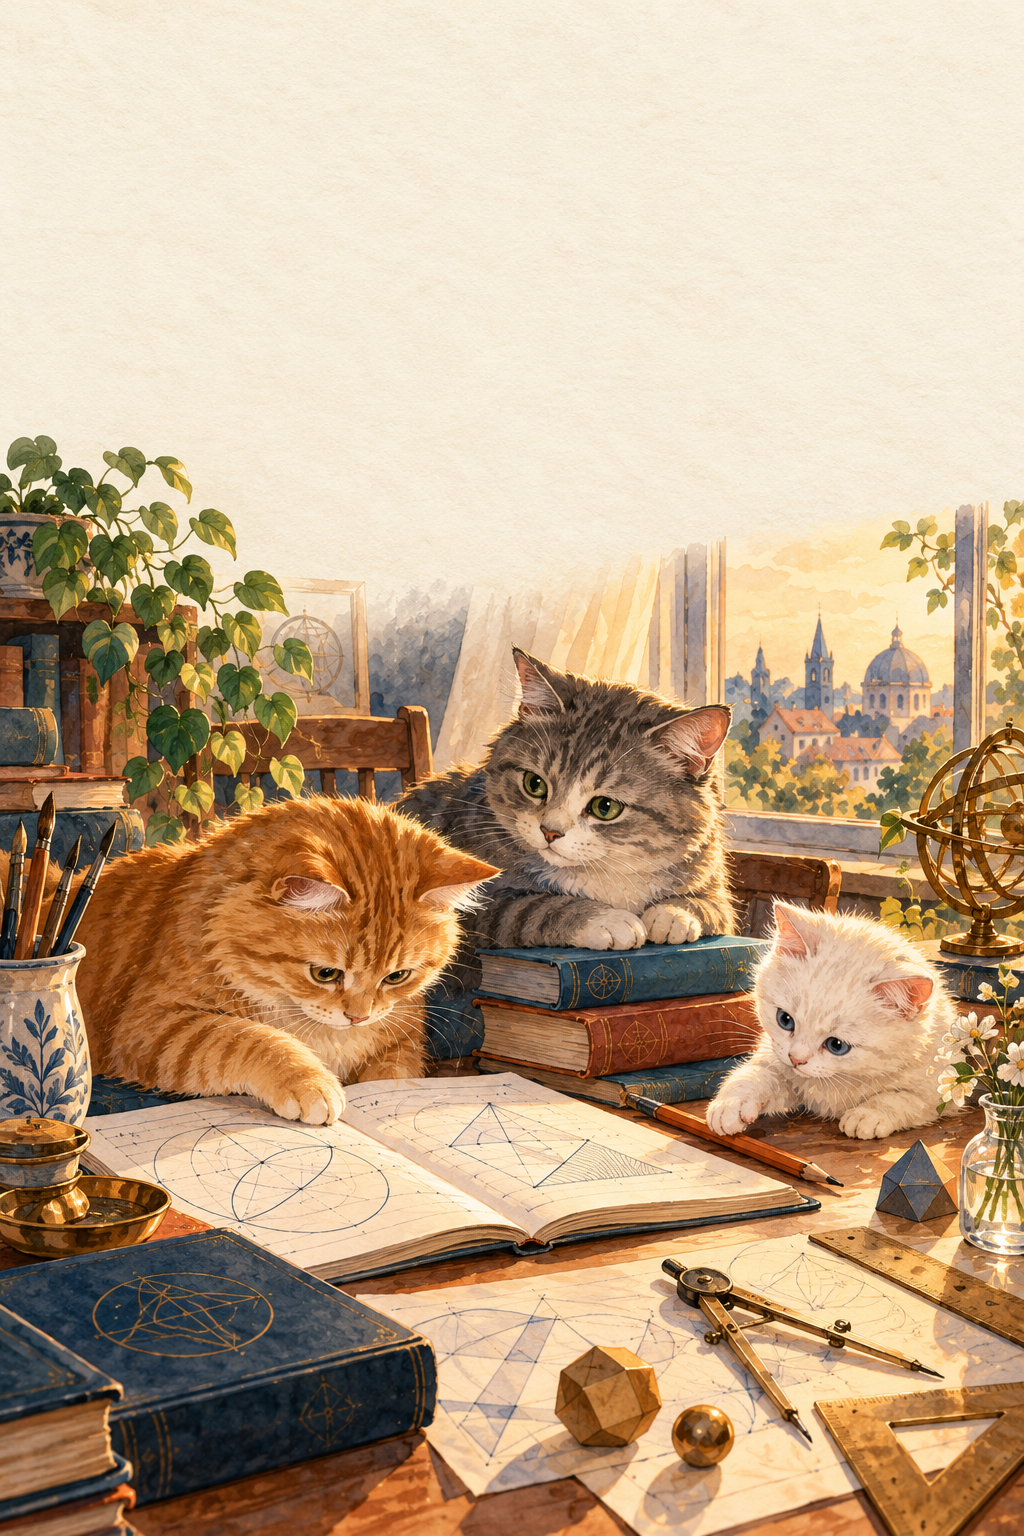
\includegraphics[width=\paperwidth,height=\paperheight]{images/cover-cats.png}};
\node[anchor=north,text width=.86\paperwidth,align=center,text=Navy] at ([yshift=-23mm]current page.north){\fontsize{29}{36}\selectfont\bfseries Алгебра перед\\математическим\\анализом\\[7mm]{\fontsize{25}{30}\selectfont для Насти}};
\node[anchor=north,text width=.8\paperwidth,align=center,text=Navy] at ([yshift=-93mm]current page.north){\large От аксиом Пеано до функций и доказательств};
\end{tikzpicture}\null\end{titlepage}
\catdecortrue
\frontmatter
\hypersetup{pageanchor=true}
\chapter*{Как читать эту книгу}
\addcontentsline{toc}{chapter}{Как читать эту книгу}
Эта книга начинается с устройства натуральных чисел и постепенно переходит к алгебре, комбинаторике, последовательностям и функциям. Здесь 16 глав и 385 задач с ответами. Определения сопровождаются английскими терминами, теоремы — доказательствами. Звёздочка \starmark{} отмечает повышенную сложность.

Сначала прочитай определения и примеры, затем попробуй решить задачи самостоятельно. Дроби сокращай до несократимого вида; в уравнениях находи все допустимые корни. В заданиях на доказательство нескольких численных проверок недостаточно. Ответы в конце помогут проверить вычисления и ход рассуждения.

Изображения в теории показывают точные графики; художественные иллюстрации не заменяют математические условия. В рисунках к задачам длины и масштабы задаются подписями.
\begingroup\small\linespread{1}\selectfont\setlength{\parskip}{0pt}\tableofcontents\endgroup
\chapter*{Справочник обозначений}\markright{Обозначения}
\addcontentsline{toc}{chapter}{Справочник обозначений}
\begingroup\small\renewcommand{\arraystretch}{1.35}\setlength{\tabcolsep}{4pt}\arrayrulecolor{Teal}\setlength{\arrayrulewidth}{.35pt}
\Needspace{7\baselineskip}\section*{Начертания символов}
\begin{longtable}{|>{\raggedright\arraybackslash}p{.21\textwidth}|>{\raggedright\arraybackslash}p{.27\textwidth}|>{\raggedright\arraybackslash}p{.46\textwidth}|}
\hline\textbf{Обозначение}&\textbf{Как читать}&\textbf{Значение}\\\hline\endfirsthead
\hline\textbf{Обозначение}&\textbf{Как читать}&\textbf{Значение}\\\hline\endhead
\hline\endfoot
\hline\endlastfoot
\(\displaystyle x\)&математический курсив&Обычное начертание переменных; смысл буквы задаётся в тексте.\\\hline
\(\displaystyle \mathrm{x}\)&прямое начертание&Так оформляют названия операторов и единицы измерения; начертание само по себе не задаёт значение.\\\hline
\(\displaystyle \symbf v=\vec v\)&полужирное начертание; стрелка&Две распространённые записи вектора.\\\hline
\(\displaystyle \mathbb R\)&двойное начертание&Распространено для числовых множеств; здесь показан знак действительных чисел.\\\hline
\(\displaystyle \mathcal A\)&каллиграфическое начертание&Часто обозначает семейство множеств или другой специально определённый объект.\\\hline
\(\displaystyle \mathfrak g\)&фрактура&Используется в алгебре для отличия одних объектов от других; смысл устанавливает определение.\\\hline
\end{longtable}
\Needspace{7\baselineskip}\section*{Числа и числовые множества}
\begin{longtable}{|>{\raggedright\arraybackslash}p{.21\textwidth}|>{\raggedright\arraybackslash}p{.27\textwidth}|>{\raggedright\arraybackslash}p{.46\textwidth}|}
\hline\textbf{Обозначение}&\textbf{Как читать}&\textbf{Значение}\\\hline\endfirsthead
\hline\textbf{Обозначение}&\textbf{Как читать}&\textbf{Значение}\\\hline\endhead
\hline\endfoot
\hline\endlastfoot
\(\displaystyle 0\)&ноль&Нейтральный элемент сложения: \(a+0=a\).\\\hline
\(\displaystyle 1\)&единица&Нейтральный элемент умножения: \(a\cdot1=a\).\\\hline
\(\displaystyle \mathbb N\)&натуральные числа&\(\{1,2,3,\ldots\}\).\\\hline
\(\displaystyle \mathbb N_0\)&натуральные числа с нулём&\(\{0,1,2,3,\ldots\}\).\\\hline
\(\displaystyle \mathbb Z\)&целые числа&\(\{\ldots,-2,-1,0,1,2,\ldots\}\).\\\hline
\(\displaystyle \mathbb Q\)&рациональные числа&Числа \(\frac pq\), где \(p\in\mathbb Z\), \(q\in\mathbb Z\), \(q\ne0\).\\\hline
\(\displaystyle \mathbb R\)&действительные числа&Числа числовой прямой, включая рациональные и иррациональные.\\\hline
\(\displaystyle \mathbb C\)&комплексные числа&Числа вида \(a+bi\), где \(a,b\in\mathbb R\).\\\hline
\(\displaystyle \mathbb H\)&кватернионы&Вещественная алгебра размерности 4 с некоммутативным ассоциативным умножением.\\\hline
\(\displaystyle \mathbb O\)&октонионы&Вещественная алгебра размерности 8; умножение не ассоциативно.\\\hline
\(\displaystyle \mathbb K\)&поле скаляров&В главах о векторных пространствах: \(\mathbb R\) или \(\mathbb C\), по условию.\\\hline
\(\displaystyle \mathbb R^n\)&эр в степени эн&Множество упорядоченных наборов из \(n\) действительных координат.\\\hline
\end{longtable}
\Needspace{7\baselineskip}\section*{Действия и сравнения чисел}
\begin{longtable}{|>{\raggedright\arraybackslash}p{.21\textwidth}|>{\raggedright\arraybackslash}p{.27\textwidth}|>{\raggedright\arraybackslash}p{.46\textwidth}|}
\hline\textbf{Обозначение}&\textbf{Как читать}&\textbf{Значение}\\\hline\endfirsthead
\hline\textbf{Обозначение}&\textbf{Как читать}&\textbf{Значение}\\\hline\endhead
\hline\endfoot
\hline\endlastfoot
\(\displaystyle +\)&плюс&Сложение: \(2+3=5\).\\\hline
\(\displaystyle -\)&минус&Вычитание или противоположное число: \(5-2=3\), \(-a\).\\\hline
\(\displaystyle \cdot\)&умножить&Умножение: \(ab=a\cdot b\).\\\hline
\(\displaystyle :\)&разделить&Деление: \(6:3=2\); делитель ненулевой.\\\hline
\(\displaystyle \frac ab\)&дробь а на б&Частное; знаменатель \(b\ne0\).\\\hline
\(\displaystyle =\)&равно&Равенство двух выражений.\\\hline
\(\displaystyle \ne\)&не равно&Выражения имеют разные значения.\\\hline
\(\displaystyle <\)&меньше&Строгое сравнение.\\\hline
\(\displaystyle >\)&больше&Строгое сравнение.\\\hline
\(\displaystyle \le\)&меньше или равно&Нестрогое сравнение; равенство допускается.\\\hline
\(\displaystyle \ge\)&больше или равно&Нестрогое сравнение; равенство допускается.\\\hline
\(\displaystyle \approx\)&приблизительно равно&Например, \(\sqrt2\approx1{,}414\).\\\hline
\(\displaystyle \pm\)&плюс или минус&\(x=\pm2\) означает \(x=-2\) или \(x=2\).\\\hline
\(\displaystyle a^n\)&а в степени эн&Степень с натуральным показателем; \(a^0=1\) при \(a\ne0\).\\\hline
\(\displaystyle a^{-n}\)&а в степени минус эн&При \(n\in\mathbb N\), \(a\ne0\): \(a^{-n}=\frac1{a^n}\).\\\hline
\(\displaystyle \sqrt a\)&квадратный корень из а&Неотрицательное число с квадратом \(a\); требуется \(a\ge0\).\\\hline
\(\displaystyle \sqrt[n]a\)&корень энной степени&Для чётного \(n\) берётся неотрицательный корень и требуется \(a\ge0\).\\\hline
\(\displaystyle |a|\)&модуль а&Расстояние от \(a\) до нуля.\\\hline
\end{longtable}
\Needspace{7\baselineskip}\section*{Делимость и сравнения по модулю}
\begin{longtable}{|>{\raggedright\arraybackslash}p{.21\textwidth}|>{\raggedright\arraybackslash}p{.27\textwidth}|>{\raggedright\arraybackslash}p{.46\textwidth}|}
\hline\textbf{Обозначение}&\textbf{Как читать}&\textbf{Значение}\\\hline\endfirsthead
\hline\textbf{Обозначение}&\textbf{Как читать}&\textbf{Значение}\\\hline\endhead
\hline\endfoot
\hline\endlastfoot
\(\displaystyle a\mathrel{\vdots}b\)&а делится на б нацело&\(a=bk\) для целого \(k\); \(b\ne0\).\\\hline
\(\displaystyle a\mid b\)&а делит б&\(b=ak\) для целого \(k\); порядок обратен записи с тремя точками.\\\hline
\(\displaystyle a\nmid b\)&а не делит б&Число \(b\) не кратно \(a\).\\\hline
\(\displaystyle \gcd(a,b)\)&наибольший общий делитель&НОД; английское greatest common divisor.\\\hline
\(\displaystyle \operatorname{lcm}(a,b)\)&наименьшее общее кратное&НОК; английское least common multiple.\\\hline
\(\displaystyle a\equiv b\pmod m\)&а сравнимо с б по модулю эм&\(m\mid(a-b)\), где \(m\) — положительное целое.\\\hline
\(\displaystyle [a]_m\)&класс а по модулю эм&Все целые числа \(a+mk\), \(k\in\mathbb Z\).\\\hline
\(\displaystyle \mathbb Z/m\mathbb Z\)&целые по модулю эм&Множество классов вычетов по модулю \(m\).\\\hline
\end{longtable}
\Needspace{7\baselineskip}\section*{Множества и пары}
\begin{longtable}{|>{\raggedright\arraybackslash}p{.21\textwidth}|>{\raggedright\arraybackslash}p{.27\textwidth}|>{\raggedright\arraybackslash}p{.46\textwidth}|}
\hline\textbf{Обозначение}&\textbf{Как читать}&\textbf{Значение}\\\hline\endfirsthead
\hline\textbf{Обозначение}&\textbf{Как читать}&\textbf{Значение}\\\hline\endhead
\hline\endfoot
\hline\endlastfoot
\(\displaystyle x\in A\)&икс принадлежит а&\(x\) — элемент множества \(A\).\\\hline
\(\displaystyle x\notin A\)&икс не принадлежит а&\(x\) не является элементом \(A\).\\\hline
\(\displaystyle \{\ldots\}\)&множество перечисленных элементов&Фигурные скобки: \(\{1,2,3\}\).\\\hline
\(\displaystyle \varnothing\)&пустое множество&Множество без элементов.\\\hline
\(\displaystyle A\subseteq B\)&а является подмножеством б&Каждый элемент \(A\) принадлежит \(B\); равенство допускается.\\\hline
\(\displaystyle A\subset B\)&а — собственное подмножество б&\(A\subseteq B\), но \(A\ne B\).\\\hline
\(\displaystyle A\cup B\)&объединение а и б&Элементы хотя бы одного из множеств.\\\hline
\(\displaystyle A\cap B\)&пересечение а и б&Элементы, принадлежащие обоим множествам.\\\hline
\(\displaystyle A\setminus B\)&разность а и б&Элементы \(A\), не принадлежащие \(B\).\\\hline
\(\displaystyle A^c\)&дополнение а&\(U\setminus A\); зависит от выбранного универсума.\\\hline
\(\displaystyle A\triangle B\)&симметрическая разность&Элементы ровно одного из двух множеств.\\\hline
\(\displaystyle A\times B\)&декартово произведение&Все упорядоченные пары с первой координатой из \(A\), второй из \(B\).\\\hline
\(\displaystyle (a,b)\)&упорядоченная пара&Порядок координат важен.\\\hline
\(\displaystyle \mathcal P(A)=2^A\)&множество всех подмножеств а&Все множества \(B\), для которых \(B\subseteq A\).\\\hline
\(\displaystyle |A|\)&число элементов а&Для конечного множества; смысл отличается от модуля числа.\\\hline
\end{longtable}
\Needspace{7\baselineskip}\section*{Промежутки числовой прямой}
\begin{longtable}{|>{\raggedright\arraybackslash}p{.21\textwidth}|>{\raggedright\arraybackslash}p{.27\textwidth}|>{\raggedright\arraybackslash}p{.46\textwidth}|}
\hline\textbf{Обозначение}&\textbf{Как читать}&\textbf{Значение}\\\hline\endfirsthead
\hline\textbf{Обозначение}&\textbf{Как читать}&\textbf{Значение}\\\hline\endhead
\hline\endfoot
\hline\endlastfoot
\(\displaystyle (a;b)\)&открытый интервал&\(a<x<b\); концы исключены.\\\hline
\(\displaystyle [a;b]\)&отрезок&\(a\le x\le b\); оба конца включены.\\\hline
\(\displaystyle [a;b)\)&полуинтервал&\(a\le x<b\); левый конец включён, правый исключён.\\\hline
\(\displaystyle (a;b]\)&полуинтервал&\(a<x\le b\); левый конец исключён, правый включён.\\\hline
\(\displaystyle \infty\)&бесконечность&Не действительное число; у бесконечной границы промежутка ставят круглую скобку.\\\hline
\end{longtable}
\Needspace{7\baselineskip}\section*{Логика и доказательства}
\begin{longtable}{|>{\raggedright\arraybackslash}p{.21\textwidth}|>{\raggedright\arraybackslash}p{.27\textwidth}|>{\raggedright\arraybackslash}p{.46\textwidth}|}
\hline\textbf{Обозначение}&\textbf{Как читать}&\textbf{Значение}\\\hline\endfirsthead
\hline\textbf{Обозначение}&\textbf{Как читать}&\textbf{Значение}\\\hline\endhead
\hline\endfoot
\hline\endlastfoot
\(\displaystyle \forall\)&для любого&Квантор всеобщности.\\\hline
\(\displaystyle \exists\)&существует&Квантор существования.\\\hline
\(\displaystyle \to,\ \Rightarrow\)&импликация&Если \(P\) истинно, то \(Q\) истинно.\\\hline
\(\displaystyle \leftrightarrow,\ \Longleftrightarrow\)&тогда и только тогда&Каждое утверждение следует из другого.\\\hline
\(\displaystyle \neg P\)&не пэ&Отрицание утверждения \(P\).\\\hline
\(\displaystyle P\land Q\)&пэ и ку&Оба утверждения истинны.\\\hline
\(\displaystyle P\lor Q\)&пэ или ку&Хотя бы одно утверждение истинно.\\\hline
\(\displaystyle \blacksquare\)&конец доказательства&В конце доказательства; в отдельных заданиях пустой квадрат может обозначать неизвестную цифру.\\\hline
\(\displaystyle \ast\)&звёздочка&Задача повышенной сложности.\\\hline
\(\displaystyle P\oplus Q\)&исключающее или&Истинно, когда истинно ровно одно из двух утверждений.\\\hline
\(\displaystyle P\uparrow Q\)&штрих Шеффера&Отрицание конъюнкции: \(\neg(P\land Q)\).\\\hline
\(\displaystyle P\downarrow Q\)&стрелка Пирса&Отрицание дизъюнкции: \(\neg(P\lor Q)\).\\\hline
\(\displaystyle \top\)&истина&Логическая константа истины.\\\hline
\(\displaystyle \bot\)&ложь&Логическая константа лжи.\\\hline
\(\displaystyle \Gamma\vdash A\)&из гаммы выводится а&Синтаксическая выводимость в указанной системе правил.\\\hline
\(\displaystyle \Gamma\models A\)&из гаммы семантически следует а&При каждой оценке, делающей все посылки истинными, заключение истинно.\\\hline
\(\displaystyle A\equiv B\)&формулы а и б равносильны&Формулы имеют одно истинностное значение при каждой оценке.\\\hline
\(\displaystyle v\models A\)&оценка вэ удовлетворяет а&Формула \(A\) истинна при оценке \(v\).\\\hline
\end{longtable}
\Needspace{7\baselineskip}\section*{Суммы, комбинаторика и последовательности}
\begin{longtable}{|>{\raggedright\arraybackslash}p{.21\textwidth}|>{\raggedright\arraybackslash}p{.27\textwidth}|>{\raggedright\arraybackslash}p{.46\textwidth}|}
\hline\textbf{Обозначение}&\textbf{Как читать}&\textbf{Значение}\\\hline\endfirsthead
\hline\textbf{Обозначение}&\textbf{Как читать}&\textbf{Значение}\\\hline\endhead
\hline\endfoot
\hline\endlastfoot
\(\displaystyle S(n)\)&следующее за эн&Операция следования в аксиомах Пеано; \(S(0)=1\).\\\hline
\(\displaystyle \sum_{k=1}^{n}a_k\)&сумма по ка от одного до эн&\(a_1+\cdots+a_n\).\\\hline
\(\displaystyle \prod_{k=1}^{n}a_k\)&произведение по ка&\(a_1\cdots a_n\).\\\hline
\(\displaystyle n!\)&эн факториал&\(1\cdot2\cdots n\) при \(n\ge1\); отдельно \(0!=1\).\\\hline
\(\displaystyle P_n\)&число перестановок&Перестановки \(n\) различных элементов: \(n!\).\\\hline
\(\displaystyle A_n^k\)&число размещений&Выбор \(k\) из \(n\) различных объектов с учётом порядка.\\\hline
\(\displaystyle \binom nk=C_n^k\)&число сочетаний из эн по ка&Выбор \(k\) из \(n\) без учёта порядка.\\\hline
\(\displaystyle a_n\)&энный член последовательности&Значение последовательности с номером \(n\).\\\hline
\(\displaystyle S_n\)&энная частичная сумма&Сумма первых \(n\) членов последовательности.\\\hline
\(\displaystyle \lim_{n\to\infty}a_n\)&предел последовательности&Число, к которому члены становятся сколь угодно близки при больших \(n\).\\\hline
\(\displaystyle \sup A\)&точная верхняя грань а&Наименьшая из верхних границ множества \(A\), если она существует.\\\hline
\(\displaystyle \inf A\)&точная нижняя грань а&Наибольшая из нижних границ непустого множества \(A\), если она существует.\\\hline
\end{longtable}
\Needspace{7\baselineskip}\section*{Функции, экспонента и логарифмы}
\begin{longtable}{|>{\raggedright\arraybackslash}p{.21\textwidth}|>{\raggedright\arraybackslash}p{.27\textwidth}|>{\raggedright\arraybackslash}p{.46\textwidth}|}
\hline\textbf{Обозначение}&\textbf{Как читать}&\textbf{Значение}\\\hline\endfirsthead
\hline\textbf{Обозначение}&\textbf{Как читать}&\textbf{Значение}\\\hline\endhead
\hline\endfoot
\hline\endlastfoot
\(\displaystyle f:X\to Y\)&эф из икс в игрек&Отображение с областью определения \(X\) и множеством назначения \(Y\).\\\hline
\(\displaystyle x\mapsto f(x)\)&икс переходит в эф от икс&Правило, сопоставляющее аргументу значение функции.\\\hline
\(\displaystyle f(x)\)&эф от икс&Значение функции при аргументе \(x\).\\\hline
\(\displaystyle f\circ g\)&композиция эф и жэ&\((f\circ g)(x)=f(g(x))\); сначала выполняется \(g\).\\\hline
\(\displaystyle f^{-1}\)&обратная функция&Обратное отображение; обычно это не \(\frac1f\).\\\hline
\(\displaystyle e\)&число е&Основание натурального логарифма; \(e=\lim_{n\to\infty}(1+\frac1n)^n\).\\\hline
\(\displaystyle e^x=\exp x\)&экспонента от икс&Показательная функция с основанием \(e\).\\\hline
\(\displaystyle \ln x=\log_e x\)&натуральный логарифм&Логарифм по основанию \(e\); \(x>0\).\\\hline
\(\displaystyle \log_a x\)&логарифм икс по основанию а&\(a>0\), \(a\ne1\), \(x>0\).\\\hline
\end{longtable}
\Needspace{7\baselineskip}\section*{Тригонометрические и гиперболические функции}
\begin{longtable}{|>{\raggedright\arraybackslash}p{.21\textwidth}|>{\raggedright\arraybackslash}p{.27\textwidth}|>{\raggedright\arraybackslash}p{.46\textwidth}|}
\hline\textbf{Обозначение}&\textbf{Как читать}&\textbf{Значение}\\\hline\endfirsthead
\hline\textbf{Обозначение}&\textbf{Как читать}&\textbf{Значение}\\\hline\endhead
\hline\endfoot
\hline\endlastfoot
\(\displaystyle \pi\)&число пи&Отношение длины окружности к её диаметру.\\\hline
\(\displaystyle \sin x\)&синус икс&Вертикальная координата на единичной окружности.\\\hline
\(\displaystyle \cos x\)&косинус икс&Горизонтальная координата на единичной окружности.\\\hline
\(\displaystyle \operatorname{tg} x\)&тангенс икс&\(\frac{\sin x}{\cos x}\) при \(\cos x\ne0\).\\\hline
\(\displaystyle \arcsin x\)&арксинус икс&Обратная к синусу на \([-\frac\pi2;\frac\pi2]\).\\\hline
\(\displaystyle \arccos x\)&арккосинус икс&Обратная к косинусу на \([0;\pi]\).\\\hline
\(\displaystyle \operatorname{arctg} x\)&арктангенс икс&Обратная к тангенсу на \((-\frac\pi2;\frac\pi2)\).\\\hline
\(\displaystyle \operatorname{sh} x\)&гиперболический синус&\(\frac{e^x-e^{-x}}2\).\\\hline
\(\displaystyle \operatorname{ch} x\)&гиперболический косинус&\(\frac{e^x+e^{-x}}2\).\\\hline
\(\displaystyle \operatorname{ctg}x\)&котангенс икс&\(\frac{\cos x}{\sin x}\); \(\sin x\ne0\).\\\hline
\(\displaystyle \operatorname{th}x\)&гиперболический тангенс&\(\frac{\operatorname{sh}x}{\operatorname{ch}x}\); определён при всех действительных \(x\).\\\hline
\(\displaystyle \operatorname{cth}x\)&гиперболический котангенс&\(\frac{\operatorname{ch}x}{\operatorname{sh}x}\); \(x\ne0\).\\\hline
\end{longtable}
\Needspace{7\baselineskip}\section*{Векторы и матрицы}
\begin{longtable}{|>{\raggedright\arraybackslash}p{.21\textwidth}|>{\raggedright\arraybackslash}p{.27\textwidth}|>{\raggedright\arraybackslash}p{.46\textwidth}|}
\hline\textbf{Обозначение}&\textbf{Как читать}&\textbf{Значение}\\\hline\endfirsthead
\hline\textbf{Обозначение}&\textbf{Как читать}&\textbf{Значение}\\\hline\endhead
\hline\endfoot
\hline\endlastfoot
\(\displaystyle \lVert v\rVert\)&длина вектора вэ&Евклидова длина, например \(\sqrt{x^2+y^2}\) для \(v=(x,y)\).\\\hline
\(\displaystyle a_{ij}\)&элемент а с индексами и, жэ&Элемент матрицы в строке \(i\), столбце \(j\).\\\hline
\(\displaystyle AB\)&произведение матриц а и б&Определено, если число столбцов \(A\) равно числу строк \(B\).\\\hline
\(\displaystyle I_n\)&единичная матрица порядка эн&На главной диагонали стоят единицы, остальные элементы равны нулю.\\\hline
\(\displaystyle \det A\)&определитель матрицы а&Для \(A=\begin{pmatrix}a&b\\c&d\end{pmatrix}\) равен \(ad-bc\).\\\hline
\(\displaystyle A^{-1}\)&обратная матрица&\(AA^{-1}=A^{-1}A=I\); существует не у всякой квадратной матрицы.\\\hline
\(\displaystyle \symbf 0\)&нулевой вектор&Вектор, все координаты которого равны нулю.\\\hline
\(\displaystyle \langle u,v\rangle=u\cdot v\)&скалярное произведение векторов&Евклидово скалярное произведение в \(\mathbb R^n\): \(\sum_{k=1}^nu_kv_k\).\\\hline
\(\displaystyle \operatorname{rank} A\)&ранг матрицы а&Число ведущих элементов в ступенчатом виде матрицы.\\\hline
\(\displaystyle \operatorname{span}S\)&линейная оболочка&Все конечные линейные комбинации векторов из указанного набора.\\\hline
\(\displaystyle \dim V\)&размерность вэ&Число векторов в базисе конечномерного пространства.\\\hline
\(\displaystyle [v]_B\)&координаты вэ в базисе бэ&Столбец коэффициентов разложения вектора по указанному базису.\\\hline
\(\displaystyle \ker T\)&ядро тэ&Векторы \(v\), для которых \(T(v)=0\).\\\hline
\(\displaystyle \operatorname{im}T\)&образ тэ&Все значения \(T(v)\).\\\hline
\(\displaystyle \mathcal P_m\)&пространство многочленов&Многочлены степени не выше \(m\), включая нулевой многочлен.\\\hline
\(\displaystyle A^{\mathrm T}\)&транспонированная матрица&Строки и столбцы меняются местами.\\\hline
\(\displaystyle \operatorname{diag}(\ldots)\)&диагональная матрица&Указанные элементы на диагонали, нули вне диагонали.\\\hline
\(\displaystyle \chi_A(t)\)&характеристический многочлен&В главе 27 используется соглашение \(\det(tI-A)\); корни — собственные значения.\\\hline
\(\displaystyle E_\lambda\)&собственное подпространство&\(\ker(A-\lambda I)\); включает нулевой вектор.\\\hline
\end{longtable}
\Needspace{7\baselineskip}\section*{Предел функции и производная}
\begin{longtable}{|>{\raggedright\arraybackslash}p{.21\textwidth}|>{\raggedright\arraybackslash}p{.27\textwidth}|>{\raggedright\arraybackslash}p{.46\textwidth}|}
\hline\textbf{Обозначение}&\textbf{Как читать}&\textbf{Значение}\\\hline\endfirsthead
\hline\textbf{Обозначение}&\textbf{Как читать}&\textbf{Значение}\\\hline\endhead
\hline\endfoot
\hline\endlastfoot
\(\displaystyle x\to a\)&икс стремится к а&Аргумент приближается к точке \(a\).\\\hline
\(\displaystyle x\to a-\)&икс стремится к а слева&Рассматриваются значения \(x<a\).\\\hline
\(\displaystyle x\to a+\)&икс стремится к а справа&Рассматриваются значения \(x>a\).\\\hline
\(\displaystyle \lim_{x\to a}f(x)\)&предел эф от икс при икс к а&Предел в точке; значение \(f(a)\) может отсутствовать или отличаться от предела.\\\hline
\(\displaystyle f'(a)\)&производная эф в точке а&Предел \(\lim_{h\to0}\frac{f(a+h)-f(a)}h\), если он существует и конечен.\\\hline
\(\displaystyle y-f(a)=f'(a)(x-a)\)&уравнение касательной&Касательная к графику дифференцируемой функции в точке с абсциссой \(a\).\\\hline
\end{longtable}
\Needspace{7\baselineskip}\section*{Алгебраические структуры}
\begin{longtable}{|>{\raggedright\arraybackslash}p{.21\textwidth}|>{\raggedright\arraybackslash}p{.27\textwidth}|>{\raggedright\arraybackslash}p{.46\textwidth}|}
\hline\textbf{Обозначение}&\textbf{Как читать}&\textbf{Значение}\\\hline\endfirsthead
\hline\textbf{Обозначение}&\textbf{Как читать}&\textbf{Значение}\\\hline\endhead
\hline\endfoot
\hline\endlastfoot
\(\displaystyle a*b\)&а звёздочка б&Результат заданной бинарной операции; это не обязательно обычное умножение.\\\hline
\(\displaystyle e_G\)&нейтральный элемент группы жэ&Элемент, не меняющий другие элементы при операции.\\\hline
\(\displaystyle a^{-1}\)&обратный к а&В группе: \(a*a^{-1}=a^{-1}*a=e\).\\\hline
\(\displaystyle \operatorname{id}_X\)&тождественное отображение икс&Оставляет каждый элемент \(X\) на месте.\\\hline
\(\displaystyle \operatorname{Sym}(X)\)&группа перестановок икс&Все биекции множества \(X\) в себя с операцией композиции.\\\hline
\(\displaystyle S_n\)&симметрическая группа степени эн&Все перестановки \(\{1,\ldots,n\}\); число элементов этой группы равно \(n!\).\\\hline
\(\displaystyle \mathrm M_2(\mathbb R)\)&матрицы два на два над эр&Кольцо действительных матриц размера \(2\times2\).\\\hline
\(\displaystyle \mathbb F_p\)&поле из пэ элементов&При простом \(p\): поле вычетов \(\mathbb Z/p\mathbb Z\).\\\hline
\end{longtable}
\Needspace{7\baselineskip}\section*{Комплексные числа}
\begin{longtable}{|>{\raggedright\arraybackslash}p{.21\textwidth}|>{\raggedright\arraybackslash}p{.27\textwidth}|>{\raggedright\arraybackslash}p{.46\textwidth}|}
\hline\textbf{Обозначение}&\textbf{Как читать}&\textbf{Значение}\\\hline\endfirsthead
\hline\textbf{Обозначение}&\textbf{Как читать}&\textbf{Значение}\\\hline\endhead
\hline\endfoot
\hline\endlastfoot
\(\displaystyle i\)&мнимая единица&Комплексное число, для которого \(i^2=-1\).\\\hline
\(\displaystyle a+bi\)&а плюс бэ и&Алгебраическая форма комплексного числа.\\\hline
\(\displaystyle \operatorname{Re}z\)&действительная часть зет&Число \(a\) в записи \(z=a+bi\).\\\hline
\(\displaystyle \operatorname{Im}z\)&мнимая часть зет&Действительное число \(b\) в записи \(z=a+bi\); множитель \(i\) в мнимую часть не входит.\\\hline
\(\displaystyle \overline z\)&зет с чертой&Комплексное сопряжение: при \(z=a+bi\) получаем \(\overline z=a-bi\).\\\hline
\(\displaystyle |z|\)&модуль комплексного числа&При \(z=a+bi\): \(\sqrt{a^2+b^2}\). Расстояние до начала координат.\\\hline
\(\displaystyle \arg z\)&аргументы зет&Все углы направления ненулевого \(z\); различаются на \(2\pi k\), \(k\in\mathbb Z\). У нуля аргумент не определён.\\\hline
\(\displaystyle \operatorname{Arg}z\)&главный аргумент зет&Для \(z\ne0\): единственный аргумент из \((-\pi;\pi]\); это принятое в книге соглашение.\\\hline
\(\displaystyle r(\cos\varphi+i\sin\varphi)\)&тригонометрическая форма&Для \(z\ne0\) здесь \(r=|z|>0\), а \(\varphi\) — один из аргументов.\\\hline
\(\displaystyle e^{i\varphi}\)&е в степени и фи&Экспоненциальная запись \(\cos\varphi+i\sin\varphi\) для действительного \(\varphi\).\\\hline
\end{longtable}
\Needspace{7\baselineskip}\section*{Кватернионы и октонионы}
\begin{longtable}{|>{\raggedright\arraybackslash}p{.21\textwidth}|>{\raggedright\arraybackslash}p{.27\textwidth}|>{\raggedright\arraybackslash}p{.46\textwidth}|}
\hline\textbf{Обозначение}&\textbf{Как читать}&\textbf{Значение}\\\hline\endfirsthead
\hline\textbf{Обозначение}&\textbf{Как читать}&\textbf{Значение}\\\hline\endhead
\hline\endfoot
\hline\endlastfoot
\(\displaystyle j\)&кватернионная единица жэ&\(j^2=-1\), \(ij=k\), \(ji=-k\).\\\hline
\(\displaystyle k\)&кватернионная единица ка&\(k=ij\), \(k^2=-1\).\\\hline
\(\displaystyle N(q)=|q|^2\)&квадрат нормы&Сумма квадратов действительных координат кватерниона или октониона.\\\hline
\(\displaystyle e_0,\ldots,e_7\)&базис октонионов&Восемь базисных элементов в выбранном соглашении; \(e_0=1\).\\\hline
\(\displaystyle [x,y,z]\)&ассоциатор&Разность \((xy)z-x(yz)\); измеряет зависимость от расстановки скобок.\\\hline
\end{longtable}
\Needspace{7\baselineskip}\section*{Метрики и окрестности}
\begin{longtable}{|>{\raggedright\arraybackslash}p{.21\textwidth}|>{\raggedright\arraybackslash}p{.27\textwidth}|>{\raggedright\arraybackslash}p{.46\textwidth}|}
\hline\textbf{Обозначение}&\textbf{Как читать}&\textbf{Значение}\\\hline\endfirsthead
\hline\textbf{Обозначение}&\textbf{Как читать}&\textbf{Значение}\\\hline\endhead
\hline\endfoot
\hline\endlastfoot
\(\displaystyle d(x,y)\)&расстояние между икс и игрек&Значение выбранной метрики; её правило задаётся в условии.\\\hline
\(\displaystyle d_1(x,y)\)&метрика суммы модулей&\(\sum_j|x_j-y_j|\).\\\hline
\(\displaystyle d_2(x,y)\)&евклидова метрика&\(\sqrt{\sum_j(x_j-y_j)^2}\).\\\hline
\(\displaystyle d_\infty(x,y)\)&метрика максимума&\(\max_j|x_j-y_j|\).\\\hline
\(\displaystyle B_r(a)\)&открытый шар&Точки \(x\), для которых \(d(x,a)<r\), где \(r>0\).\\\hline
\(\displaystyle (x_{n_k})\)&подпоследо\-вательность&Члены с номерами \(n_1<n_2<\cdots\).\\\hline
\end{longtable}
\Needspace{7\baselineskip}\section*{Интегралы и ряды}
\begin{longtable}{|>{\raggedright\arraybackslash}p{.21\textwidth}|>{\raggedright\arraybackslash}p{.27\textwidth}|>{\raggedright\arraybackslash}p{.46\textwidth}|}
\hline\textbf{Обозначение}&\textbf{Как читать}&\textbf{Значение}\\\hline\endfirsthead
\hline\textbf{Обозначение}&\textbf{Как читать}&\textbf{Значение}\\\hline\endhead
\hline\endfoot
\hline\endlastfoot
\(\displaystyle \int_a^b f(x)\,dx\)&определённый интеграл&Интеграл от нижней границы до верхней.\\\hline
\(\displaystyle \int f(x)\,dx\)&неопределённый интеграл&Семейство первообразных на указанном интервале.\\\hline
\(\displaystyle [F(x)]_a^b\)&подстановка пределов&Разность \(F(b)-F(a)\).\\\hline
\(\displaystyle \|P\|\)&мелкость разбиения&Наибольшая длина его частей; смысл отличается от нормы вектора.\\\hline
\(\displaystyle L(f,P)\)&нижняя сумма Дарбу&\(\sum_i m_i(x_i-x_{i-1})\); используются инфимумы на частях.\\\hline
\(\displaystyle U(f,P)\)&верхняя сумма Дарбу&\(\sum_i M_i(x_i-x_{i-1})\); используются супремумы на частях.\\\hline
\(\displaystyle \sum_{n=1}^\infty a_n\)&числовой ряд&Предел конечных частичных сумм, если он существует и конечен.\\\hline
\(\displaystyle \textstyle\sum_{n=0}^\infty c_n(x-a)^n\)&степенной ряд&Для каждого фиксированного аргумента получается числовой ряд.\\\hline
\end{longtable}
\endgroup

\mainmatter
\chapter{Числа и свойства арифметических действий}\markright{Глава 1}
\section*{Натуральные числа: аксиомы Пеано}

Вычисления с натуральными числами опираются на небольшое число исходных положений.
Такое исходное положение называют \term{аксиомой} (axiom): в выбранной теории его принимают без доказательства,
а дальнейшие утверждения из него выводят.

\begin{definition}
\term{Натуральные числа с нулём} (natural numbers including zero) образуют множество \(\mathbb N_0\).
Для его описания выделяют начальное число \(0\) и операцию \(S\),
где \(S(n)\) означает число, следующее за \(n\).
Тройка \((\mathbb N_0,0,S)\) удовлетворяет следующим аксиомам Пеано.
\end{definition}

Запись \(n\in\mathbb N_0\) означает, что \(n\) принадлежит множеству \(\mathbb N_0\).
Буквы \(m,n\) в аксиомах обозначают произвольные его элементы.

\begin{axiom}[Начальный элемент]
\(0\in\mathbb N_0\).
\end{axiom}

\begin{axiom}[Следующее число]
Для каждого \(n\in\mathbb N_0\) определено единственное следующее число \(S(n)\in\mathbb N_0\).
\end{axiom}

\begin{axiom}[У нуля нет предшественника]
Для любого \(n\in\mathbb N_0\) выполнено \(S(n)\ne0\).
\end{axiom}

\begin{axiom}[Разные числа имеют разные следующие числа]
Если \(S(m)=S(n)\), то \(m=n\).
\end{axiom}

Последняя аксиома выражает \term{инъективность} (injectivity) операции \(S\):
равенство результатов возможно только при равенстве исходных чисел.

\begin{axiom}[Принцип математической индукции]
Пусть \(P(n)\) --- утверждение, сформулированное для \(n\in\mathbb N_0\).
Если
\begin{enumerate}[label=\arabic*.,leftmargin=2em,itemsep=3pt]
\item утверждение \(P(0)\) истинно;
\item для любого \(n\in\mathbb N_0\) из истинности \(P(n)\) следует истинность \(P(S(n))\),
\end{enumerate}
то \(P(n)\) истинно для всех \(n\in\mathbb N_0\).
\end{axiom}

\par\addvspace{5pt}\begin{lrbox}{\CatFlowBox}\begin{minipage}[t]{\linewidth}
\setlength{\parskip}{5pt}\setlength{\columnsep}{4.5mm}\setlength{\intextsep}{0pt}
\begin{wrapfigure}[13]{l}{54mm}
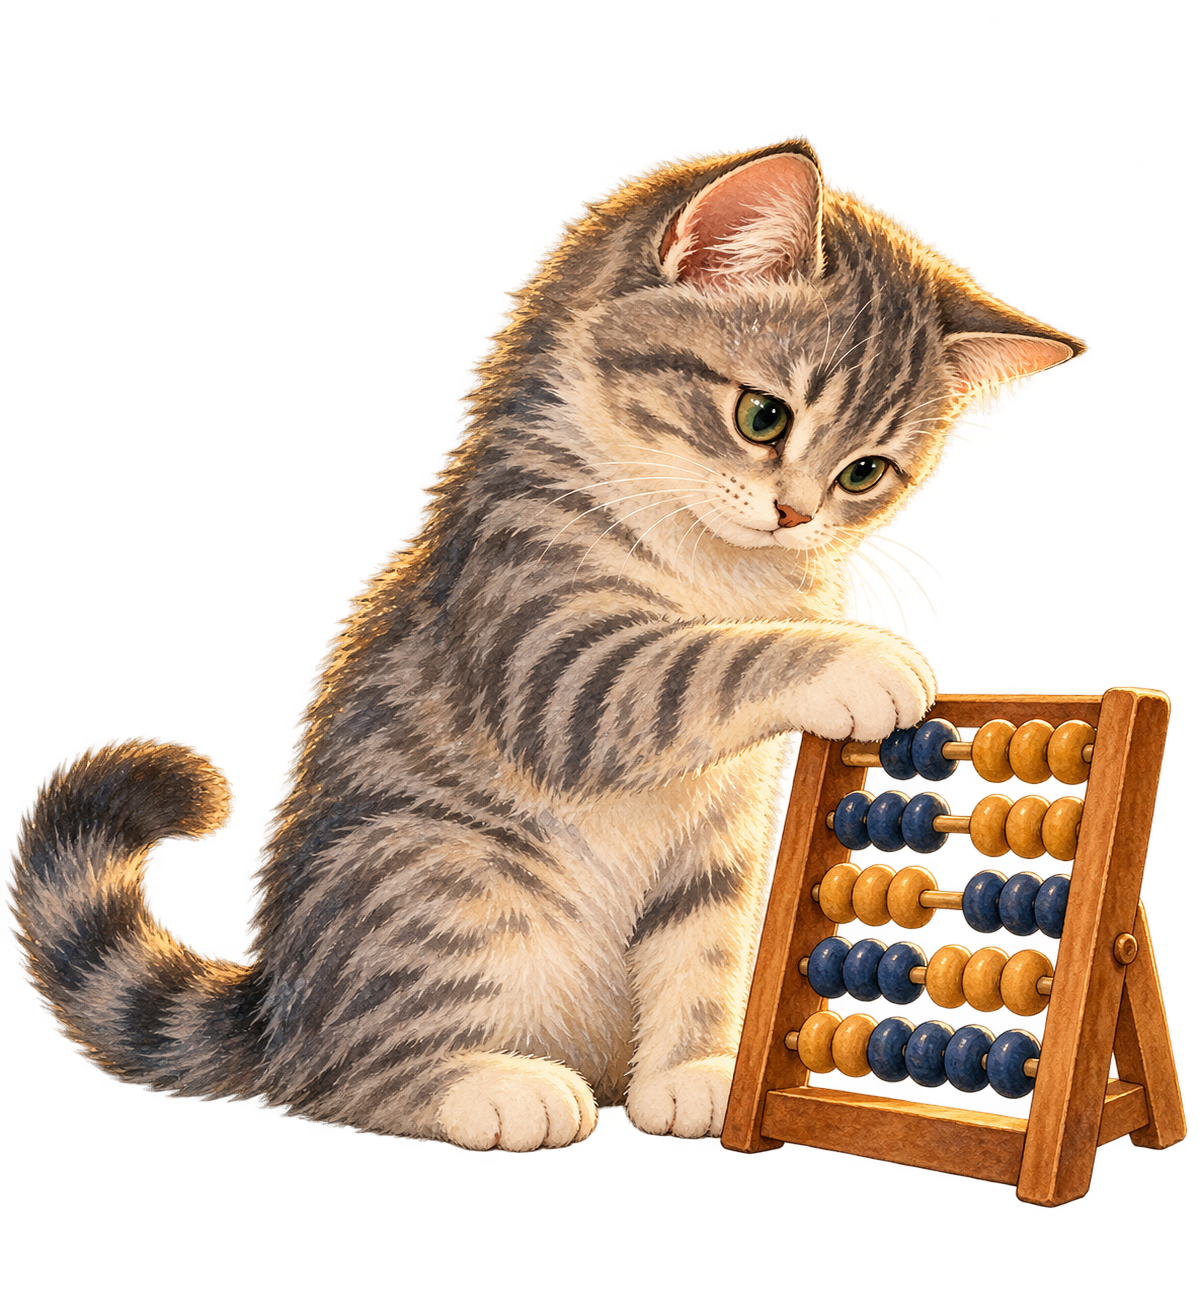
\includegraphics[width=54mm,height=58mm,keepaspectratio]{images/unique/art-02.png}
\end{wrapfigure}
В доказательстве методом \term{математической индукции} (mathematical induction)
первый пункт называют \term{базой индукции} (base case),
а второй --- \term{индукционным переходом} (inductive step).
Внутри перехода истинность \(P(n)\) временно принимают как
\term{индукционное предположение} (induction hypothesis) и из неё выводят следующий случай.
Проверка нескольких примеров не заменяет переход для произвольного \(n\).
\par\WFclear\end{minipage}\end{lrbox}%
\ifdim\dimexpr\ht\CatFlowBox+\dp\CatFlowBox\relax<64mm\dp\CatFlowBox=\dimexpr64mm-\ht\CatFlowBox\relax\fi%
\noindent\usebox{\CatFlowBox}\par\addvspace{5pt}
\begin{definition}
\term{Единица} (one) --- число \(1=S(0)\).
Далее обозначают \(2=S(1)\), \(3=S(2)\) и так далее.
\end{definition}

По аксиоме об отсутствии предшественника нуля \(1\ne0\).
Таким образом, привычная запись множества имеет вид
\[
\mathbb N_0=\{0,1,2,3,\ldots\}.
\]

\begin{definition}
\term{Натуральные числа} (natural numbers) в этом сборнике --- элементы множества
\[
\mathbb N=\mathbb N_0\setminus\{0\}=\{1,2,3,\ldots\}.
\]
Знак \(\setminus\) означает удаление указанных элементов: здесь из \(\mathbb N_0\) удалён ноль.
\end{definition}

Натуральные числа используют для счёта отдельных предметов.
Ноль соответствует отсутствию предметов, единица --- одному предмету.
В литературе встречается и соглашение \(0\in\mathbb N\), поэтому принятая здесь договорённость указана явно.

\section*{Как из следования получаются сложение и умножение}

\begin{definition}
\term{Рекурсивное определение} (recursive definition) задаёт начальное значение
и правило получения следующего значения из уже определённого.
Для \(a,b\in\mathbb N_0\) сложение и умножение задают правилами
\[
\begin{aligned}
a+0&=a, & a+S(b)&=S(a+b),\\
a\cdot0&=0, & a\cdot S(b)&=a\cdot b+a.
\end{aligned}
\]
\end{definition}

Например,
\[
a+1=a+S(0)=S(a+0)=S(a).
\]
Поэтому после введения сложения вместо \(S(n)\) можно писать \(n+1\).
В индукционном переходе тогда доказывают \(P(n+1)\), предполагая \(P(n)\).
Если утверждение сформулировано только для \(n\ge1\), базой служит случай \(n=1\).

Следующие два доказательства показывают, как привычные свойства действий выводятся из определений.

\begin{theorem}[Ноль слева при сложении]
Для любого \(n\in\mathbb N_0\) выполнено \(0+n=n\).
\end{theorem}

\begin{proof}
База: при \(n=0\) рекурсивное определение даёт \(0+0=0\).
Переход: предположим, что \(0+n=n\). Тогда
\[
0+S(n)=S(0+n)=S(n).
\]
Значит, утверждение верно и для следующего числа. По принципу индукции оно верно для всех \(n\in\mathbb N_0\).
\end{proof}

Теперь рекурсивное правило умножения даёт
\[
a\cdot1=a\cdot S(0)=a\cdot0+a=0+a=a.
\]

\begin{theorem}[Ассоциативность сложения]
Для любых \(a,b,c\in\mathbb N_0\)
\[
(a+b)+c=a+(b+c).
\]
\end{theorem}

\par\addvspace{5pt}\begin{lrbox}{\CatFlowBox}\begin{minipage}[t]{\linewidth}
\setlength{\parskip}{5pt}\setlength{\columnsep}{4.5mm}\setlength{\intextsep}{0pt}
\begin{wrapfigure}[13]{l}{54mm}

\includegraphics[width=54mm,height=58mm,keepaspectratio]{images/unique/art-04.png}
\end{wrapfigure}
\textit{Доказательство.} Зафиксируем произвольные \(a,b\in\mathbb N_0\) и проведём индукцию по \(c\).
База \(c=0\):
\[
(a+b)+0=a+b=a+(b+0).
\]
Предположим, что \((a+b)+c=a+(b+c)\). По рекурсивному правилу сложения
\[
\begin{aligned}
(a+b)+S(c)
&=S\bigl((a+b)+c\bigr)\\
&=S\bigl(a+(b+c)\bigr)\\
&=a+S(b+c)\\
&=a+\bigl(b+S(c)\bigr).
\end{aligned}
\]
Переход доказан. Принцип индукции завершает доказательство.\hfill\(\square\)
\par\WFclear\end{minipage}\end{lrbox}%
\ifdim\dimexpr\ht\CatFlowBox+\dp\CatFlowBox\relax<64mm\dp\CatFlowBox=\dimexpr64mm-\ht\CatFlowBox\relax\fi%
\noindent\usebox{\CatFlowBox}\par\addvspace{5pt}


\begin{definition}
\term{Целые числа} (\emph{integers}) --- натуральные числа, противоположные им отрицательные числа и ноль:
\[
\mathbb Z=\{\ldots,-3,-2,-1,0,1,2,3,\ldots\}.
\]
\end{definition}

\begin{definition}
\term{Противоположное число} (\emph{additive inverse}) к числу \(a\) --- число \(-a\), сумма которого с \(a\) равна нулю:
\[
a+(-a)=0.
\]
Например, \(5\) и \(-5\) противоположны; число, противоположное нулю, --- сам ноль.
\end{definition}

На числовой прямой число тем больше, чем правее находится его точка.
Например, \(-8<-3<0<4\).
Запись \(a\in\mathbb Z\) читается: «\(a\) принадлежит множеству целых чисел».

\section*{Действия с целыми числами}

Сумма, разность и произведение целых чисел всегда являются целыми числами.
Деление может вывести за пределы целых чисел: например, \(6:3=2\), но \(1:2\) не является целым числом.

Вычитание означает прибавление противоположного числа:
\[
a-b=a+(-b),\qquad a-(-b)=a+b.
\]
При сложении двух отрицательных чисел складывают их расстояния до нуля и ставят минус:
\[
(-7)+(-5)=-12.
\]
При сложении чисел разных знаков из большего расстояния до нуля вычитают меньшее
и берут знак числа, расположенного дальше от нуля:
\[
-14+9=-5,\qquad -9+14=5,\qquad -9+9=0.
\]
При умножении или делении двух ненулевых чисел одинаковые знаки дают плюс, разные --- минус:
\[
(-6)(-4)=24,\qquad (-6)\cdot4=-24,\qquad
\frac{-24}{-6}=4,\qquad \frac{24}{-6}=-4.
\]
Деление на ноль не определено; в частности, запись \(\frac{0}{0}\) также не имеет значения.

\section*{От целых чисел к рациональным}

\begin{definition}
\term{Рациональное число} (\emph{rational number}) --- число, которое можно записать в виде
\[
\frac pq,\qquad p\in\mathbb Z,\quad q\in\mathbb Z,\quad q\ne0.
\]
Множество рациональных чисел обозначают \(\mathbb Q\).
\end{definition}

Любое целое число рационально, поскольку \(n=\frac n1\).
Например, \(3\), \(-2\), \(0\), \(\frac12\) и \(-\frac34\) --- рациональные числа.
Правила действий с дробями подробно разобраны в главе 3.
Следующие свойства удобно сформулировать сразу для всех рациональных чисел:
ими пользуются и при вычислениях, и при дальнейших преобразованиях выражений с буквами.

\section*{Основные свойства арифметических действий}

Во всех формулах ниже \(a,b,c\) --- произвольные рациональные числа.

\textbf{Замкнутость сложения и умножения.}
Сумма и произведение рациональных чисел снова рациональны:
\[
a+b\in\mathbb Q,\qquad ab\in\mathbb Q.
\]
Разность также рациональна; частное рационально при ненулевом делителе.

\par\addvspace{5pt}\begin{lrbox}{\CatFlowBox}\begin{minipage}[t]{\linewidth}
\setlength{\parskip}{5pt}\setlength{\columnsep}{4.5mm}\setlength{\intextsep}{0pt}
\begin{wrapfigure}[9]{r}{54mm}
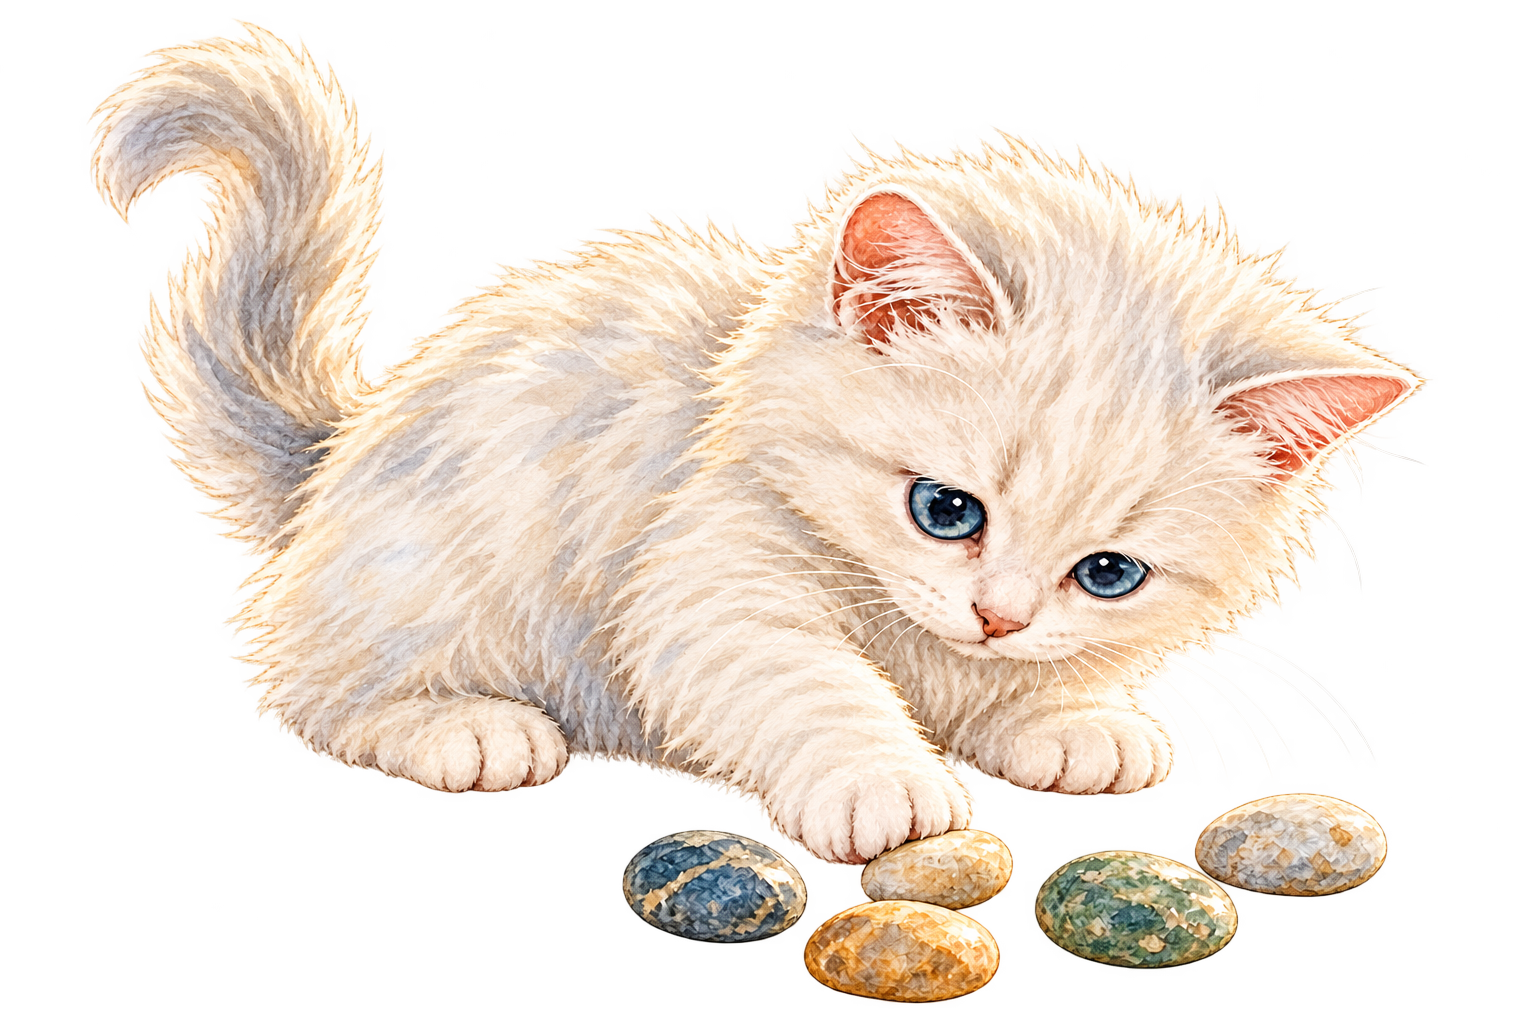
\includegraphics[width=54mm,height=58mm,keepaspectratio]{images/unique/art-03.png}
\end{wrapfigure}
\textbf{Коммутативность} (переместительный закон).
Перестановка слагаемых или множителей не меняет результата:
\[
a+b=b+a,\qquad ab=ba.
\]

\textbf{Ассоциативность} (сочетательный закон).
Группировка слагаемых или множителей не меняет результата:
\[
(a+b)+c=a+(b+c),\qquad (ab)c=a(bc).
\]

\textbf{Нейтральные элементы.}
Прибавление нуля и умножение на единицу не меняют число:
\[
a+0=0+a=a,\qquad a\cdot1=1\cdot a=a.
\]
Поэтому \(0\) называют нейтральным элементом сложения,
а \(1\) --- нейтральным элементом умножения.
\par\WFclear\end{minipage}\end{lrbox}%
\ifdim\dimexpr\ht\CatFlowBox+\dp\CatFlowBox\relax<64mm\dp\CatFlowBox=\dimexpr64mm-\ht\CatFlowBox\relax\fi%
\noindent\usebox{\CatFlowBox}\par\addvspace{5pt}
\textbf{Противоположное число.}
У каждого числа есть противоположное:
\[
a+(-a)=(-a)+a=0.
\]

\begin{definition}
\term{Обратное число} (\emph{multiplicative inverse; reciprocal}) к ненулевому числу \(a\) --- число \(\frac1a\),
произведение которого с \(a\) равно единице:
\[
a\cdot\frac1a=\frac1a\cdot a=1,\qquad a\ne0.
\]
\end{definition}
Например, \(2\) и \(\frac12\) взаимно обратны.
У нуля обратного числа нет. Деление заменяется умножением на обратное число:
\[
\frac ab=a\cdot\frac1b,\qquad b\ne0.
\]

\textbf{Дистрибутивность} (распределительный закон).
Умножение распределяется относительно сложения:
\[
a(b+c)=ab+ac,\qquad (a+b)c=ac+bc.
\]
Для разности соответственно \(a(b-c)=ab-ac\).

\textbf{Умножение на ноль и правила знаков.}
Из перечисленных свойств следуют равенства
\[
a\cdot0=0,\qquad (-a)b=-(ab),\qquad (-a)(-b)=ab.
\]

\textbf{Законы сокращения.}
Прибавление одного числа к обеим частям равенства можно отменить;
умножение можно отменить, если общий множитель ненулевой:
\[
a+c=b+c\ \Longrightarrow\ a=b,
\]
\[
ac=bc,\quad c\ne0\ \Longrightarrow\ a=b.
\]
Знак \(\Longrightarrow\) означает «из этого следует».

\textbf{Свойство нулевого произведения.}
Произведение равно нулю тогда и только тогда, когда хотя бы один множитель равен нулю:
\[
ab=0\quad\Longleftrightarrow\quad a=0\ \text{или}\ b=0.
\]
Знак \(\Longleftrightarrow\) означает, что утверждения равносильны: каждое следует из другого.

Коммутативность и ассоциативность относятся к сложению и умножению.
Переносить их на вычитание и деление нельзя:
\[
7-2\ne2-7,\qquad (12:3):2\ne12:(3:2).
\]

\section*{Порядок действий}

\begin{enumerate}[label=\arabic*.,leftmargin=2em,itemsep=3pt]
\item Действия в скобках, начиная с самых внутренних.
\item Возведение в степень. Например, \(3^2=3\cdot3\).
\item Умножение и деление --- слева направо.
\item Сложение и вычитание --- слева направо.
\end{enumerate}

Степень относится только к своему основанию:
\[
(-3)^2=9,\qquad -3^2=-(3^2)=-9.
\]
Например,
\[
-3-(-5)\cdot2=-3-(-10)=-3+10=7.
\]

\section*{Порядок на числовой прямой}
Для любых рациональных \(a,b\) выполняется ровно одно из условий: \(a<b\), \(a=b\), \(a>b\).
Если \(a<b\) и \(b<c\), то \(a<c\) — это \textbf{транзитивность}.
Из \(a<b\) следует \(a+c<b+c\). Если также \(c>0\), то \(ac<bc\); если \(c<0\), то \(ac>bc\).
Эти правила объясняют преобразования неравенств в главе 11.
\Needspace{7\baselineskip}\section*{Задачи}
\begingroup\setlength{\parskip}{3pt}
\noindent\begin{minipage}[t]{\linewidth}\textbf{1.1.} Сравни: \(- 8\) и \(- 3;\allowbreak 0\) и \(- 5;\allowbreak - 4\) и \(4\).\par\end{minipage}\par
\noindent\begin{minipage}[t]{\linewidth}\textbf{1.2.} Вычисли: \(- 7 + (- 5)\).\par\end{minipage}\par
\noindent\begin{minipage}[t]{\linewidth}\textbf{1.3.} Вычисли: \(- 14 + 9 + 8\).\par\end{minipage}\par
\noindent\begin{minipage}[t]{\linewidth}\textbf{1.4.} Вычисли: \(6 - (- 4) - 13\).\par\end{minipage}\par
\noindent\begin{minipage}[t]{\linewidth}\textbf{1.5.} Вычисли: \((- 6) \cdot  (- 4) : (- 3)\).\par\end{minipage}\par
\noindent\begin{minipage}[t]{\linewidth}\textbf{1.6.} Вычисли: \(0 \cdot  (- 15) + 0 : (- 3) + 7\). Можно ли вычислить \(7 : 0\)?\par\end{minipage}\par
\noindent\begin{minipage}[t]{\linewidth}\textbf{1.7.} Вычисли: \(18 - 4 \cdot  7 + 12 : (- 3)\).\par\end{minipage}\par
\noindent\begin{minipage}[t]{\linewidth}\textbf{1.8.} Вычисли: \(48 : (- 6) \cdot  2 - 9 + 5\).\par\end{minipage}\par
\par\addvspace{5pt}\begin{lrbox}{\CatFlowBox}\begin{minipage}[t]{\linewidth}
\setlength{\parskip}{5pt}\setlength{\columnsep}{4.5mm}\setlength{\intextsep}{0pt}
\begin{wrapfigure}[9]{r}{54mm}
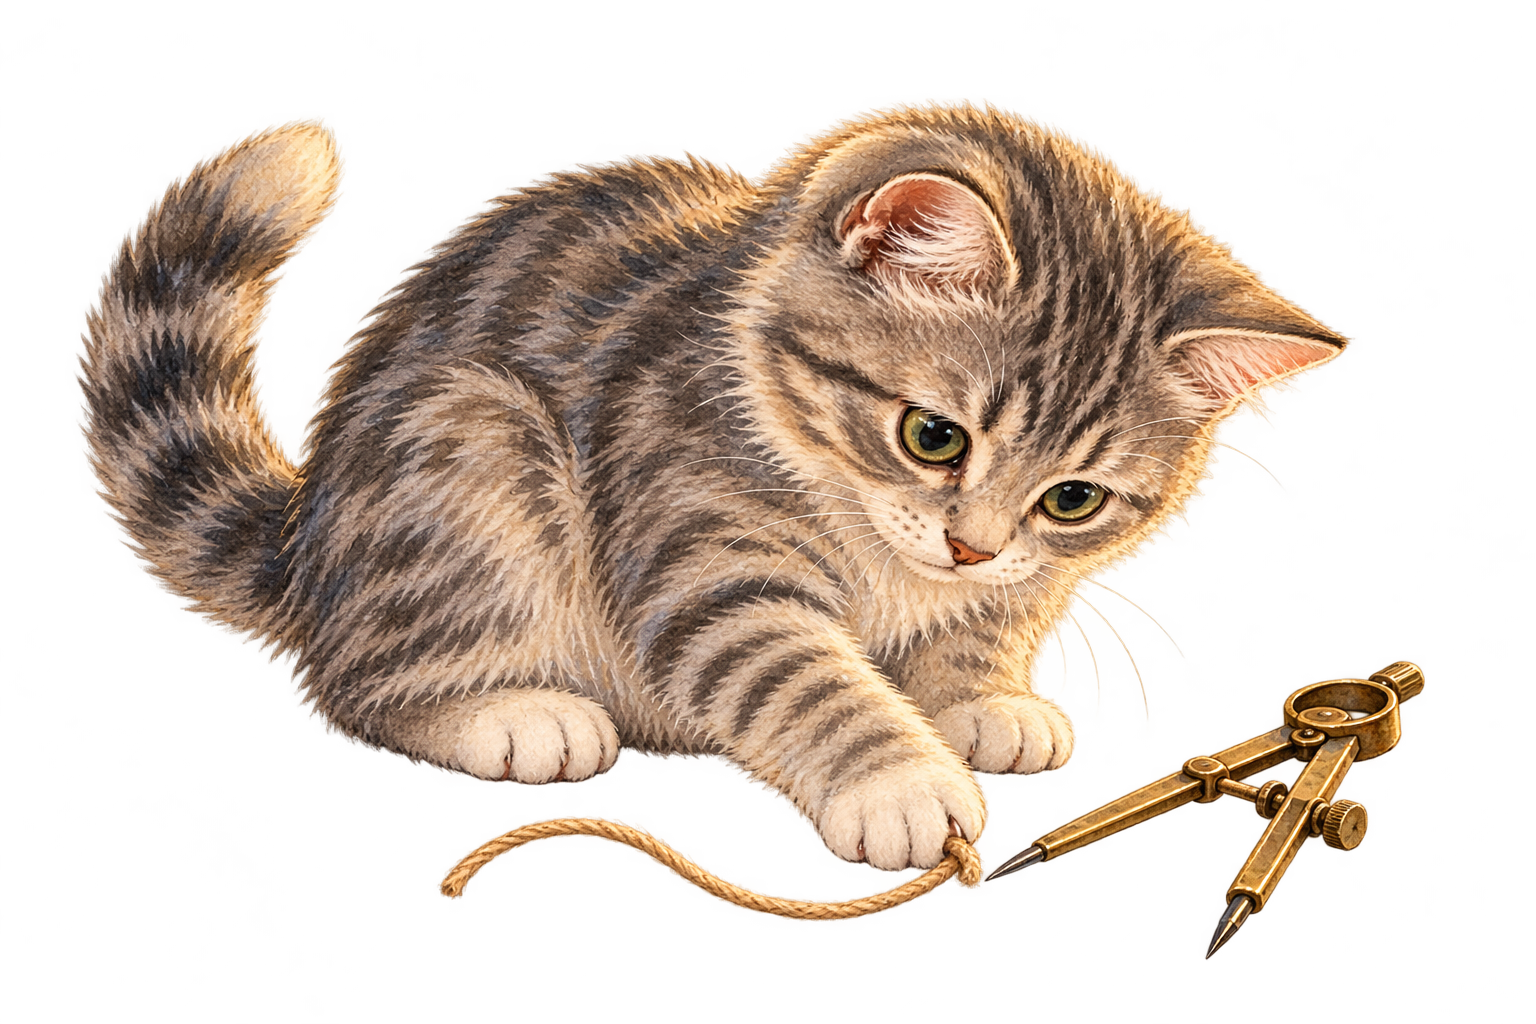
\includegraphics[width=54mm,height=58mm,keepaspectratio]{images/unique/art-05.png}
\end{wrapfigure}
\textbf{1.9.} Вычисли: \(- 3 \cdot  [8 - (5 - 9)] + 10\).\par

\textbf{1.10.} Вычисли: \((- 3)^{2} - 3^{2} + (- 2)^{3} - (- 2^{2})\).\par

\textbf{1.11.} Из жизни. Утром было \(- 6 {}^{\circ} C\). К полудню потеплело на \(9 {}^{\circ} C\), а вечером похолодало на \(5 {}^{\circ} C\). Какая температура стала вечером?\par

\textbf{1.12.} Из жизни. Лифт находился на уровне \(- 2\) подземной парковки, поднялся на \(7\) уровней и опустился на \(3\). На каком уровне он оказался? Уровень земли обозначен \(0\), уровни идут подряд.\par

\textbf{1.13.} Из жизни. На игровом счёте было \(120\) очков. За каждую из трёх ошибок сняли \(15\) очков, затем начислили \(40\) очков. Сколько очков осталось?\par

\textbf{1.14.}\starmark{} Вычисли: \(- 48 : [6 - 2 \cdot  (- 1)] + 3 \cdot  [- 4 - (- 7)]\).\par

\textbf{1.15.}\starmark{} Подставь скобки в \(18 - 6 : 3 + 1\), сохранив порядок чисел и действий, чтобы получилось \(3\).\par
\par\WFclear\end{minipage}\end{lrbox}%
\ifdim\dimexpr\ht\CatFlowBox+\dp\CatFlowBox\relax<64mm\dp\CatFlowBox=\dimexpr64mm-\ht\CatFlowBox\relax\fi%
\noindent\usebox{\CatFlowBox}\par\addvspace{5pt}

\noindent\begin{minipage}[t]{\linewidth}\textbf{1.16.}\starmark{} В викторине за верный ответ дают \(5\) очков, за неверный снимают \(3\). Участник ответил на все \(12\) вопросов и набрал \(28\) очков. Сколько было верных ответов?\par\end{minipage}\par
\noindent\begin{minipage}[t]{\linewidth}\textbf{1.17.} Докажи математической индукцией, что \(\sum_{k=1}^{n}k=\dfrac{n(n+1)}2\) для всех \(n\in\mathbb N_0\). Знак \(\sum\) обозначает сумму слагаемых при указанных значениях индекса; при \(n=0\) сумма пуста и равна \(0\).\par\end{minipage}\par
\noindent\begin{minipage}[t]{\linewidth}\textbf{1.18.} Докажи математической индукцией: \(1+3+\cdots+(2n-1)=n^2\) для всех \(n\in\mathbb N\).\par\end{minipage}\par
\noindent\begin{minipage}[t]{\linewidth}\textbf{1.19.}\starmark{} Докажи математической индукцией: \(\sum_{k=1}^{n}k^2=\dfrac{n(n+1)(2n+1)}6\) для всех \(n\in\mathbb N_0\). Пустая сумма равна нулю.\par\end{minipage}\par
\noindent\begin{minipage}[t]{\linewidth}\textbf{1.20.} Докажи математической индукцией: \(\sum_{k=0}^{n}2^k=2^{n+1}-1\) для всех \(n\in\mathbb N_0\). Здесь \(2^0=1\).\par\end{minipage}\par
\noindent\begin{minipage}[t]{\linewidth}\textbf{1.21.} Докажи математической индукцией: \(3^n\ge2n+1\) для всех \(n\in\mathbb N_0\). Здесь \(3^0=1\).\par\end{minipage}\par
\noindent\begin{minipage}[t]{\linewidth}\textbf{1.22.} Докажи математической индукцией: \(2^n\ge n^2\) для всех целых \(n\ge4\).\par\end{minipage}\par
\noindent\begin{minipage}[t]{\linewidth}\textbf{1.23.}\starmark{} Докажи математической индукцией: \(\sum_{k=1}^{n}k^3=\left(\dfrac{n(n+1)}2\right)^2\) для всех \(n\in\mathbb N_0\). Пустая сумма равна нулю.\par\end{minipage}\par
\noindent\begin{minipage}[t]{\linewidth}\textbf{1.24.}\starmark{} Докажи индукцией по натуральному \(n\) неравенство Бернулли: \((1+x)^n\ge1+nx\) для любого рационального \(x\ge-1\). Объясни, почему условие \(1+x\ge0\) нужно в индукционном переходе.\par\end{minipage}\par
\noindent\begin{minipage}[t]{\linewidth}\textbf{1.25.} Докажи единственность противоположного рационального числа: если \(a+x=0\) и \(a+y=0\), то \(x=y\). Используй свойства сложения.\par\end{minipage}\par
\noindent\begin{minipage}[t]{\linewidth}\textbf{1.26.} Докажи свойство нулевого произведения для рациональных чисел: \(ab=0\) тогда и только тогда, когда \(a=0\) или \(b=0\).\par\end{minipage}\par
\endgroup

\chapter{Делимость, простые числа, НОД и НОК}
\section*{Делимость и кратность}

\begin{definition}
\term{Делимость нацело} (\emph{divisibility}): целое число \(b\) делится на целое число \(a\ne0\),
если существует целое число \(k\), для которого
\[
b=ak.
\]
При этом \(a\) называют \term{делителем} (\emph{divisor}) числа \(b\).
\end{definition}

Запись с тремя вертикальными точками \(b\mathrel{\vdots}a\) читается:
«\(b\) делится на \(a\) нацело».
В университетских курсах также используют запись \(a\mid b\): «\(a\) делит \(b\)».
Порядок чисел в этих двух обозначениях противоположен:
\[
12\mathrel{\vdots}4\quad\Longleftrightarrow\quad4\mid12,
\qquad 12=4\cdot3.
\]
Здесь знак \(\Longleftrightarrow\) означает, что записи выражают одно и то же утверждение.

\begin{definition}
\term{Кратное} (\emph{multiple}) числа \(a\ne0\) --- целое число \(b\), которое можно представить как \(b=ak\)
с целым \(k\). Иначе говоря, \(b\) кратно \(a\), если \(b\mathrel{\vdots}a\).
\end{definition}

Например, положительные кратные числа \(4\): \(4,8,12,16,\ldots\).
Ноль также кратен любому ненулевому целому числу: \(0=a\cdot0\).
В задачах на НОК рассматриваются только \emph{положительные} общие кратные.

\section*{Простые и составные числа}

\begin{definition}
\term{Простое число} (\emph{prime number}) --- натуральное число, имеющее ровно два положительных делителя:
\(1\) и само это число.
\end{definition}

\begin{definition}
\term{Составное число} (\emph{composite number}) --- натуральное число больше \(1\), имеющее положительный делитель,
отличный от \(1\) и от самого числа.
\end{definition}

Число \(7\) простое: его положительные делители --- \(1\) и \(7\).
Число \(9\) составное: кроме \(1\) и \(9\), оно делится на \(3\).
Число \(1\) не является ни простым, ни составным.
Число \(2\) --- единственное чётное простое число.

\section*{Наибольший общий делитель и наименьшее общее кратное}

\begin{definition}
\term{Наибольший общий делитель} (\emph{greatest common divisor, gcd}) положительных целых чисел \(a\) и \(b\) ---
наибольшее положительное целое число, на которое оба числа делятся нацело.
Обозначения: \(\text{НОД}(a,b)\) и \(\gcd(a,b)\).
Английское название --- \emph{greatest common divisor}, сокращённо \emph{gcd}.
\end{definition}

Общие положительные делители чисел \(12\) и \(18\) --- \(1,2,3,6\), поэтому
\[
\text{НОД}(12,18)=\gcd(12,18)=6.
\]

\begin{definition}
\term{Наименьшее общее кратное} (\emph{least common multiple, lcm}) положительных целых чисел \(a\) и \(b\) ---
наименьшее положительное целое число, которое делится нацело и на \(a\), и на \(b\).
Обозначения: \(\text{НОК}(a,b)\) и \(\operatorname{lcm}(a,b)\).
Английское название --- \emph{least common multiple}, сокращённо \emph{lcm}.
\end{definition}

Положительные общие кратные чисел \(12\) и \(18\) --- \(36,72,108,\ldots\), поэтому
\[
\text{НОК}(12,18)=\operatorname{lcm}(12,18)=36.
\]

\begin{definition}
\term{Взаимно простые числа} (\emph{coprime integers}) --- положительные целые числа, НОД которых равен \(1\).
\end{definition}
Например, \(8\) и \(15\) взаимно просты, хотя оба числа составные.

\section*{Основная теорема арифметики (ОТА)}

\begin{theorem}
Каждое натуральное число больше \(1\) можно представить произведением простых чисел.
Такое разложение единственно с точностью до перестановки множителей.
\end{theorem}
\begin{proof}Существование докажем индукцией по числу: простое число уже разложено; составное имеет вид \(ab\), где \(1<a,b<n\), и к обоим множителям применяется предположение индукции. Для единственности используем следующий факт: если простое \(p\) делит \(ab\), то оно делит \(a\) или \(b\). Если \(p\nmid a\), то \(\gcd(p,a)=1\); обратная подстановка в алгоритме Евклида даёт целые \(u,v\) с \(up+va=1\). Умножение на \(b\) показывает, что \(p\mid b\). Теперь первый простой множитель одного разложения обязан совпасть с одним из множителей другого; сократим его и повторим. Все множители совпадут с точностью до порядка.\end{proof}

Например,
\[
60=2\cdot2\cdot3\cdot5=2^2\cdot3\cdot5.
\]
Множители \(2,3,5\) простые; запись \(60=4\cdot15\) ещё не является разложением на простые множители.

\section*{Вычисление НОД и НОК по разложению}

Разложите каждое число на простые множители, объединив повторения в степени.
Для НОД возьмите только общие простые множители в \emph{меньших} степенях.
Для НОК возьмите все встречающиеся простые множители в \emph{больших} степенях.
Если общих простых множителей нет, НОД равен \(1\).

Например,
\[
12=2^2\cdot3,\qquad18=2\cdot3^2,
\]
\[
\gcd(12,18)=2\cdot3=6,\qquad
\operatorname{lcm}(12,18)=2^2\cdot3^2=36.
\]
Для нескольких положительных чисел правило такое же:
в НОД входят множители, общие \emph{всем} числам, с наименьшими показателями;
в НОК --- все встретившиеся множители с наибольшими показателями.

\begin{theorem}
Для любых положительных целых чисел \(a,b\)
\[
\gcd(a,b)\operatorname{lcm}(a,b)=ab.
\]
\end{theorem}
\begin{proof}Для каждого простого множителя обозначим его показатели в \(a,b\) через \(\alpha,\beta\), допуская показатель \(0\). В НОД его показатель \(\min(\alpha,\beta)\), в НОК — \(\max(\alpha,\beta)\). Их сумма равна \(\alpha+\beta\), то есть показателю того же простого в \(ab\). По единственности разложения произведения равны.\end{proof}
Это равенство относится к двум числам; напрямую переносить его на три числа нельзя.

\section*{Алгоритм Евклида}

Для нахождения НОД можно последовательно делить с остатком,
каждый раз заменяя пару «делимое, делитель» парой «делитель, остаток».
Когда остаток стал нулём, НОД равен последнему ненулевому делителю.
Например,
\[
48=2\cdot18+12,\qquad
18=1\cdot12+6,\qquad
12=2\cdot6+0,
\]
поэтому \(\gcd(48,18)=6\).

\section*{Признаки делимости}

В десятичной записи натурального числа действуют следующие признаки.
Каждый из них даёт необходимое и достаточное условие: число делится на указанный делитель
\emph{тогда и только тогда}, когда выполнена соответствующая проверка.

\begin{itemize}[leftmargin=1.5em,itemsep=4pt]
\item \textbf{На \(2\):} последняя цифра --- \(0,2,4,6\) или \(8\).
\item \textbf{На \(3\):} сумма цифр делится на \(3\).
\item \textbf{На \(4\):} число, образованное двумя последними цифрами, делится на \(4\).
\item \textbf{На \(5\):} последняя цифра --- \(0\) или \(5\).
\item \textbf{На \(6\):} число делится одновременно на \(2\) и на \(3\).
\item \textbf{На \(8\):} число, образованное тремя последними цифрами, делится на \(8\).
\item \textbf{На \(9\):} сумма цифр делится на \(9\).
\item \textbf{На \(10\):} последняя цифра --- \(0\).
\end{itemize}

Если число содержит меньше двух или трёх цифр, в признаках на \(4\) и \(8\) проверяют само число.
Например, \(123\mathrel{\vdots}3\), поскольку \(1+2+3=6\),
но \(123\) не делится на \(9\), поскольку \(6\) не делится на \(9\).
\Needspace{7\baselineskip}\section*{Задачи}
\begin{enumerate}[label={},leftmargin=3.2em,itemsep=10pt]
\Needspace{3\baselineskip}\item[\textbf{2.1.}] Выпиши все положительные делители \(36\).
\Needspace{3\baselineskip}\item[\textbf{2.2.}] Выпиши все положительные делители \(48\).
\Needspace{3\baselineskip}\item[\textbf{2.3.}] Найди общие положительные делители \(20\) и \(30\).
\Needspace{3\baselineskip}\item[\textbf{2.4.}] Выпиши кратные \(7\) между \(20\) и \(60\).
\Needspace{3\baselineskip}\item[\textbf{2.5.}] Найди наименьшее трёхзначное число, кратное \(8\).
\Needspace{3\baselineskip}\item[\textbf{2.6.}] Раздели на простые и составные: \(17,\allowbreak 25,\allowbreak 31,\allowbreak 39,\allowbreak 49,\allowbreak 51,\allowbreak 53\).
\Needspace{3\baselineskip}\item[\textbf{2.7.}] Выпиши простые числа от \(20\) до \(40\).
\Needspace{3\baselineskip}\item[\textbf{2.8.}] Может ли простое число оканчиваться на \(0\)? Объясни.
\Needspace{3\baselineskip}\item[\textbf{2.9.}] Любое ли нечётное число простое? Приведи контрпример.
\Needspace{3\baselineskip}\item[\textbf{2.10.}] Какие числа делятся на \(3\), а какие на \(9\): \(126,\allowbreak 234,\allowbreak 405,\allowbreak 517,\allowbreak 702\)?
\Needspace{3\baselineskip}\item[\textbf{2.11.}] Какие числа делятся на \(2\) и на \(5\) одновременно: \(125,\allowbreak 230,\allowbreak 342,\allowbreak 480,\allowbreak 705\)?
\Needspace{3\baselineskip}\item[\textbf{2.12.}] Какие цифры можно поставить вместо \(\square \) в \(43 \square \), чтобы число делилось на \(3\)?
\Needspace{3\baselineskip}\item[\textbf{2.13.}] Какая цифра вместо \(\square \) в \(7 \square  2\) даёт делимость на \(9\)?
\Needspace{3\baselineskip}\item[\textbf{2.14.}] Какие цифры вместо \(\square \) в \(12 \square \) дают делимость на \(2\) и на \(3\)?
\Needspace{3\baselineskip}\item[\textbf{2.15.}] Разложи \(72\) на простые множители.
\Needspace{3\baselineskip}\item[\textbf{2.16.}] Разложи \(150\) на простые множители.
\Needspace{3\baselineskip}\item[\textbf{2.17.}] Разложи \(252\) на простые множители.
\Needspace{3\baselineskip}\item[\textbf{2.18.}] Заверши разложение \(90 = 2 \cdot  5 \cdot  9\) на простые множители.
\Needspace{3\baselineskip}\item[\textbf{2.19.}] Найди НОД и НОК чисел \(24\) и \(36\).
\Needspace{3\baselineskip}\item[\textbf{2.20.}] Найди НОД и НОК чисел \(18\) и \(45\).
\Needspace{3\baselineskip}\item[\textbf{2.21.}] Найди НОД и НОК чисел \(8\) и \(15\).
\Needspace{3\baselineskip}\item[\textbf{2.22.}] Найди НОД и НОК чисел \(12,\allowbreak 18\) и \(30\).
\Needspace{3\baselineskip}\item[\textbf{2.23.}] Из \(24\) карандашей и \(36\) ручек собери максимум одинаковых наборов, использовав всё. Сколько наборов и что в каждом?
\Needspace{3\baselineskip}\item[\textbf{2.24.}] Автобусы отправились вместе в 9:00. Интервалы отправления: \(12\) и \(18\) минут. Когда следующее совместное отправление?
\Needspace{3\baselineskip}\item[\textbf{2.25.}] Прямоугольник \(60 \times  84\) см разрежь без остатка на одинаковые квадраты наибольшей стороны. Найди сторону и число квадратов.
\Needspace{3\baselineskip}\item[\textbf{2.26.}] Выпиши все положительные делители \(24\).
\Needspace{3\baselineskip}\item[\textbf{2.27.}] Выпиши первые пять положительных кратных \(6\).
\Needspace{3\baselineskip}\item[\textbf{2.28.}] Какие из чисел \(1,\allowbreak 2,\allowbreak 9,\allowbreak 13,\allowbreak 21,\allowbreak 29\) простые?
\Needspace{3\baselineskip}\item[\textbf{2.29.}] На какие числа из списка \(2,\allowbreak 3,\allowbreak 5,\allowbreak 9,\allowbreak 10\) делится \(450\)?
\Needspace{3\baselineskip}\item[\textbf{2.30.}] Разложи \(84\) на простые множители.
\Needspace{3\baselineskip}\item[\textbf{2.31.}] Найди НОД и НОК чисел \(12\) и \(18\).
\Needspace{3\baselineskip}\item[\textbf{2.32.}] Из жизни. Для праздника есть \(42\) яблока и \(56\) мандаринов. Их нужно разложить без остатка в максимальное число одинаковых подарков. Сколько подарков получится и что будет в каждом?
\Needspace{3\baselineskip}\item[\textbf{2.33.}] Из жизни. Два индикатора загорелись одновременно. Один загорается каждые \(8\) секунд, другой каждые \(12\) секунд. Через сколько секунд они впервые снова загорятся вместе?
\Needspace{3\baselineskip}\item[\textbf{2.34.}] Из жизни. В коробке \(97\) деталей. Можно ли разложить их в одинаковые группы больше одной детали, получив больше одной группы, без остатка?
\Needspace{3\baselineskip}\item[\textbf{2.35.}\starmark] Найди наименьшее натуральное число, которое при делении на \(6,\allowbreak 8\) и \(9\) даёт остаток \(1\) и при этом больше \(1\).
\Needspace{3\baselineskip}\item[\textbf{2.36.}\starmark] НОД двух положительных целых чисел равен \(6\), НОК равен \(180\). Одно число \(30\). Найди второе.
\Needspace{3\baselineskip}\item[\textbf{2.37.}\starmark] Найди все цифры \(a\) и \(b\), чтобы четырёхзначное число \(\overline{3a5b}\) делилось на \(5\) и на \(9\).
\Needspace{3\baselineskip}\item[\textbf{2.38.}] Пусть \(a>b>0\) --- целые числа. Докажи равенство \(\gcd(a,b)=\gcd(b,a-b)\), показав, что пары имеют одни и те же положительные общие делители.
\Needspace{3\baselineskip}\item[\textbf{2.39.}] Пусть \(p\) --- простое число, \(a,b\) --- положительные целые числа. Используя основную теорему арифметики, докажи: если \(p\mid ab\), то \(p\mid a\) или \(p\mid b\).
\end{enumerate}

\chapter{Обыкновенные дроби}
\begin{definition}\term{Обыкновенная дробь} (\emph{common fraction}) \(\frac{a}{b}\) — запись частного \(a : b\), где \(a\) и \(b\) — целые числа и \(b \ne  0\).\end{definition}
\begin{definition}\term{Числитель} (\emph{numerator}) дроби \(\frac{a}{b}\) — число \(a\), записанное над дробной чертой.\end{definition}
\begin{definition}\term{Знаменатель} (\emph{denominator}) дроби \(\frac{a}{b}\) — ненулевое число \(b\), записанное под дробной чертой.\end{definition}
\begin{definition}\term{Правильная положительная дробь} (\emph{proper positive fraction}) — дробь с положительными числителем и знаменателем, у которой числитель меньше знаменателя.\end{definition}
\begin{definition}\term{Неправильная положительная дробь} (\emph{improper positive fraction}) — дробь с положительными числителем и знаменателем, у которой числитель не меньше знаменателя.\end{definition}
\begin{definition}\term{Смешанное число} (\emph{mixed number}) — сумма целой части и правильной дробной части; например, \(2 \frac{1}{3} = 2 + \frac{1}{3}\).\end{definition}
\section*{Основное свойство дроби}
\(\frac{a}{b} = \frac{ak}{bk}\) при \(k \ne  0\). Числитель и знаменатель можно умножать или делить на одно и то же ненулевое число.\par
\section*{Действия с дробями}
Сложение: \(\frac{a}{b} + \frac{c}{d} = \frac{ad + bc}{bd}\), где \(b,\allowbreak d \ne  0\).\par
Вычитание: \(\frac{a}{b} - \frac{c}{d} = \frac{ad - bc}{bd}\), где \(b,\allowbreak d \ne  0\).\par
Умножение: \((\frac{a}{b}) \cdot  (\frac{c}{d}) = \frac{ac}{bd}\).\par
Деление: \((\frac{a}{b}) : (\frac{c}{d}) = \frac{ad}{bc}\); дополнительно \(c \ne  0\).\par
Сравнение при \(b,\allowbreak d > 0\): сравни \(a \cdot  d\) и \(c \cdot  b\).\par
{\small\textit{Пример: \(\frac{1}{2} + \frac{1}{3} = \frac{3}{6} + \frac{2}{6} = \frac{5}{6}\). Сокращение: \(\frac{18}{24} = \frac{3}{4}\).}}\par
\Needspace{7\baselineskip}\section*{Задачи}
\begin{enumerate}[label={},leftmargin=3.2em,itemsep=10pt]
\Needspace{3\baselineskip}\item[\textbf{3.1.}] Сократи \(\frac{18}{24}\).
\Needspace{3\baselineskip}\item[\textbf{3.2.}] Преврати \(\frac{17}{5}\) в смешанное число.
\Needspace{3\baselineskip}\item[\textbf{3.3.}] Преврати \(2 \frac{3}{7}\) в неправильную дробь.
\Needspace{3\baselineskip}\item[\textbf{3.4.}] Сравни \(\frac{5}{8}\) и \(\frac{7}{12}\).
\Needspace{3\baselineskip}\item[\textbf{3.5.}] Вычисли \(\frac{3}{4} - \frac{5}{6}\).
\Needspace{3\baselineskip}\item[\textbf{3.6.}] Вычисли \(\frac{7}{15} + \frac{2}{9}\).
\Needspace{3\baselineskip}\item[\textbf{3.7.}] Вычисли \((- \frac{3}{7}) \cdot  (\frac{14}{9})\).
\Needspace{3\baselineskip}\item[\textbf{3.8.}] Вычисли \((\frac{2}{3}) : (\frac{4}{9})\).
\Needspace{3\baselineskip}\item[\textbf{3.9.}] Вычисли \(2 \frac{1}{3} - 1 \frac{5}{6}\).
\Needspace{3\baselineskip}\item[\textbf{3.10.}] Вычисли \((\frac{1}{2} + \frac{1}{3}) : (\frac{5}{6})\).
\Needspace{3\baselineskip}\item[\textbf{3.11.}] Вычисли \(\frac{\frac{3}{4}}{\frac{9}{8}}\).
\Needspace{3\baselineskip}\item[\textbf{3.12.}] Из \(80\) страниц прочитали \(\frac{3}{5}\). Сколько страниц осталось?
\Needspace{3\baselineskip}\item[\textbf{3.13.}] Из жизни. На пирог ушло \(\frac{3}{4}\) кг муки, а на блины \(\frac{2}{3}\) кг. Сколько всего муки израсходовали?
\Needspace{3\baselineskip}\item[\textbf{3.14.}] Из жизни. В бутылке \(\frac{3}{2}\) л сока. Его разливают по стаканам вместимостью \(\frac{1}{4}\) л. Сколько полных стаканов получится?
\Needspace{3\baselineskip}\item[\textbf{3.15.}] Из жизни. Турист прошёл \(\frac{2}{5}\) маршрута длиной \(15\) км. Сколько километров ему осталось?
\Needspace{3\baselineskip}\item[\textbf{3.16.}\starmark] Вычисли: \((\frac{3}{4} - \frac{5}{6}) : (\frac{7}{9} - \frac{2}{3}) + \frac{1}{2}\).
\Needspace{3\baselineskip}\item[\textbf{3.17.}\starmark] В первый день прочитали \(\frac{1}{3}\) книги, во второй — \(\frac{2}{5}\) оставшихся страниц. После этого осталось \(72\) страницы. Сколько страниц в книге?
\Needspace{3\baselineskip}\item[\textbf{3.18.}\starmark] Бак был полон. Израсходовали \(\frac{1}{4}\) воды, затем \(\frac{1}{3}\) оставшейся. После долива \(15\) л бак снова стал полным. Какова вместимость бака?
\Needspace{3\baselineskip}\item[\textbf{3.19.}] Для целых \(a,b,c,d\), где \(b\ne0\), \(d\ne0\), докажи критерий равенства дробей: \(\frac ab=\frac cd\) тогда и только тогда, когда \(ad=bc\).
\Needspace{3\baselineskip}\item[\textbf{3.20.}] Докажи, что для любого \(n\in\mathbb N\) выполнено \(\sum_{k=1}^{n}\frac1{k(k+1)}=\frac n{n+1}\).
\end{enumerate}

\chapter{Десятичные дроби и проценты}\markright{Глава 4}
\begin{definition}\term{Десятичная дробь} (\emph{decimal}) — запись числа с разрядами десятых, сотых, тысячных и далее после запятой.\end{definition}
\begin{definition}\term{Процент} (\emph{percent}) — одна сотая часть: \(1 \% = \frac{1}{100} = 0{,}01\).\end{definition}
\begin{definition}\term{Периодическая десятичная дробь} (\emph{repeating decimal}) — бесконечная десятичная дробь с повторяющимся блоком цифр начиная с некоторого разряда.\end{definition}
\section*{Правила вычислений}
При сложении и вычитании десятичных дробей записывай одинаковые разряды друг под другом.\par
При умножении сначала умножь без запятых, затем отдели справа столько цифр, сколько их было после запятых в обоих множителях вместе.\par
При делении перенеси запятую в делимом и делителе на одинаковое число разрядов, чтобы делитель стал целым.\par
\section*{Формулы для процентов}
\(p \%\) от \(A\): \(A \cdot \frac{p}{100}\). Если \(p \%\) числа равны \(B\) и \(p \ne  0\), то число равно \(\frac{100 B}{p}\).\par
Рост на \(p \%\): \(A (1 + \frac{p}{100})\). Снижение на \(p \%\): \(A (1 - \frac{p}{100})\).\par
Процентное изменение: \(\frac{\text{новое значение} - \text{старое значение}}{\text{старое значение}} \cdot 100 \%\), если старое значение не равно \(0\). В обычных задачах о цене исходная цена положительна.\par
Каждый следующий процент изменения относится к уже изменённой величине.\par
\section*{Округление и периодические дроби}
Если следующая за оставляемым разрядом цифра \(0 - 4\), разряд не меняют; если \(5 - 9\), увеличивают на \(1\), при необходимости перенося единицу в старший разряд.\par
Любая периодическая десятичная дробь представляет рациональное число.\par
{\small\textit{Пример: \(\frac{1}{3} = 0{,}(3)\). Цена \(100\) рублей после двух скидок по \(10 \%\): \(100 \cdot 0{,}9 \cdot 0{,}9 = 81\) рубль.}}\par
\Needspace{7\baselineskip}\section*{Задачи}
\begingroup\setlength{\parskip}{3pt}
\noindent\begin{minipage}[t]{\linewidth}\textbf{4.1.} Вычисли \(3{,}75 + 0{,}086\).\par\end{minipage}\par
\noindent\begin{minipage}[t]{\linewidth}\textbf{4.2.} Вычисли \(8 - 2{,}47\).\par\end{minipage}\par
\noindent\begin{minipage}[t]{\linewidth}\textbf{4.3.} Вычисли \(0{,}24 \cdot  0{,}5\).\par\end{minipage}\par
\noindent\begin{minipage}[t]{\linewidth}\textbf{4.4.} Вычисли \(4{,}2 : 0{,}07\).\par\end{minipage}\par
\noindent\begin{minipage}[t]{\linewidth}\textbf{4.5.} Запиши \(\dfrac{7}{8}\) десятичной дробью.\par\end{minipage}\par
\par\addvspace{5pt}\begin{lrbox}{\CatFlowBox}\begin{minipage}[t]{\linewidth}
\setlength{\parskip}{5pt}\setlength{\columnsep}{4.5mm}\setlength{\intextsep}{0pt}
\begin{wrapfigure}[9]{l}{54mm}
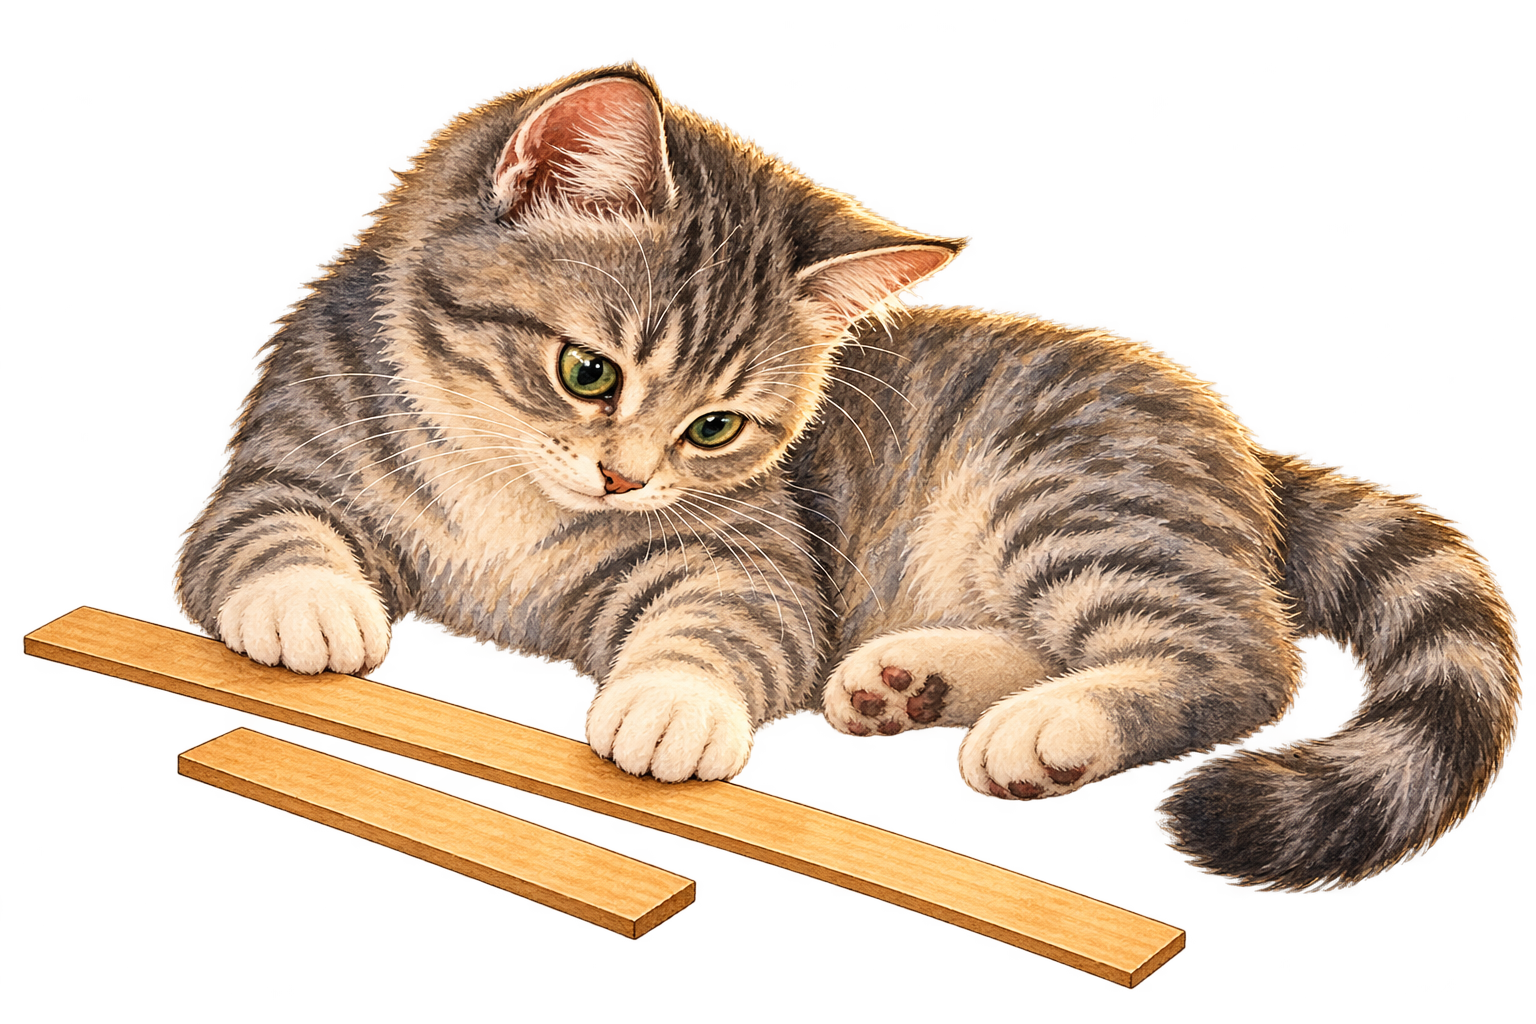
\includegraphics[width=54mm,height=58mm,keepaspectratio]{images/unique/art-14.png}
\end{wrapfigure}
\textbf{4.6.} Запиши \(0{,}125\) несократимой обыкновенной дробью.\par

\textbf{4.7.} Запиши \(\dfrac{2}{3}\) периодической десятичной дробью.\par

\textbf{4.8.} Округли \(3{,}14159\) до сотых и до тысячных.\par

\textbf{4.9.} Найди \(15 \%\) от \(240\).\par

\textbf{4.10.} \(30 \%\) числа равны \(54\). Найди число.\par

\textbf{4.11.} Цена выросла с \(800\) до \(920\) рублей. На сколько процентов?\par

\textbf{4.12.} Цену \(1000\) рублей повысили на \(20 \%\), затем снизили на \(20 \%\). Найди итоговую цену и изменение в процентах от исходной.\par
\par\WFclear\end{minipage}\end{lrbox}%
\ifdim\dimexpr\ht\CatFlowBox+\dp\CatFlowBox\relax<64mm\dp\CatFlowBox=\dimexpr64mm-\ht\CatFlowBox\relax\fi%
\noindent\usebox{\CatFlowBox}\par\addvspace{5pt}

\noindent\begin{minipage}[t]{\linewidth}\textbf{4.13.} Купили \(1{,}8\) кг яблок по \(125\) рублей за килограмм. Сколько заплатили?\par\end{minipage}\par
\noindent\begin{minipage}[t]{\linewidth}\textbf{4.14.} Куртка стоит \(4800\) рублей. Скидка составляет \(15 \%\). Какова цена со скидкой?\par\end{minipage}\par
\noindent\begin{minipage}[t]{\linewidth}\textbf{4.15.} Велосипедист проехал \(7{,}86\) км утром и \(5{,}47\) км вечером. Найди общий путь и округли его до десятых километра.\par\end{minipage}\par
\noindent\begin{minipage}[t]{\linewidth}\textbf{4.16.}\starmark{} После скидки \(20 \%\) и следующей скидки \(10 \%\) товар стоит \(2160\) рублей. Найди исходную цену.\par\end{minipage}\par
\noindent\begin{minipage}[t]{\linewidth}\textbf{4.17.}\starmark{} Цена выросла на \(25 \%\). На сколько процентов нужно снизить новую цену, чтобы получить исходную?\par\end{minipage}\par
\noindent\begin{minipage}[t]{\linewidth}\textbf{4.18.}\starmark{} Смешали \(200\) г раствора с массовой долей соли \(10 \%\) и \(300\) г раствора с долей соли \(20 \%\). Найди массовую долю соли в смеси.\begin{center}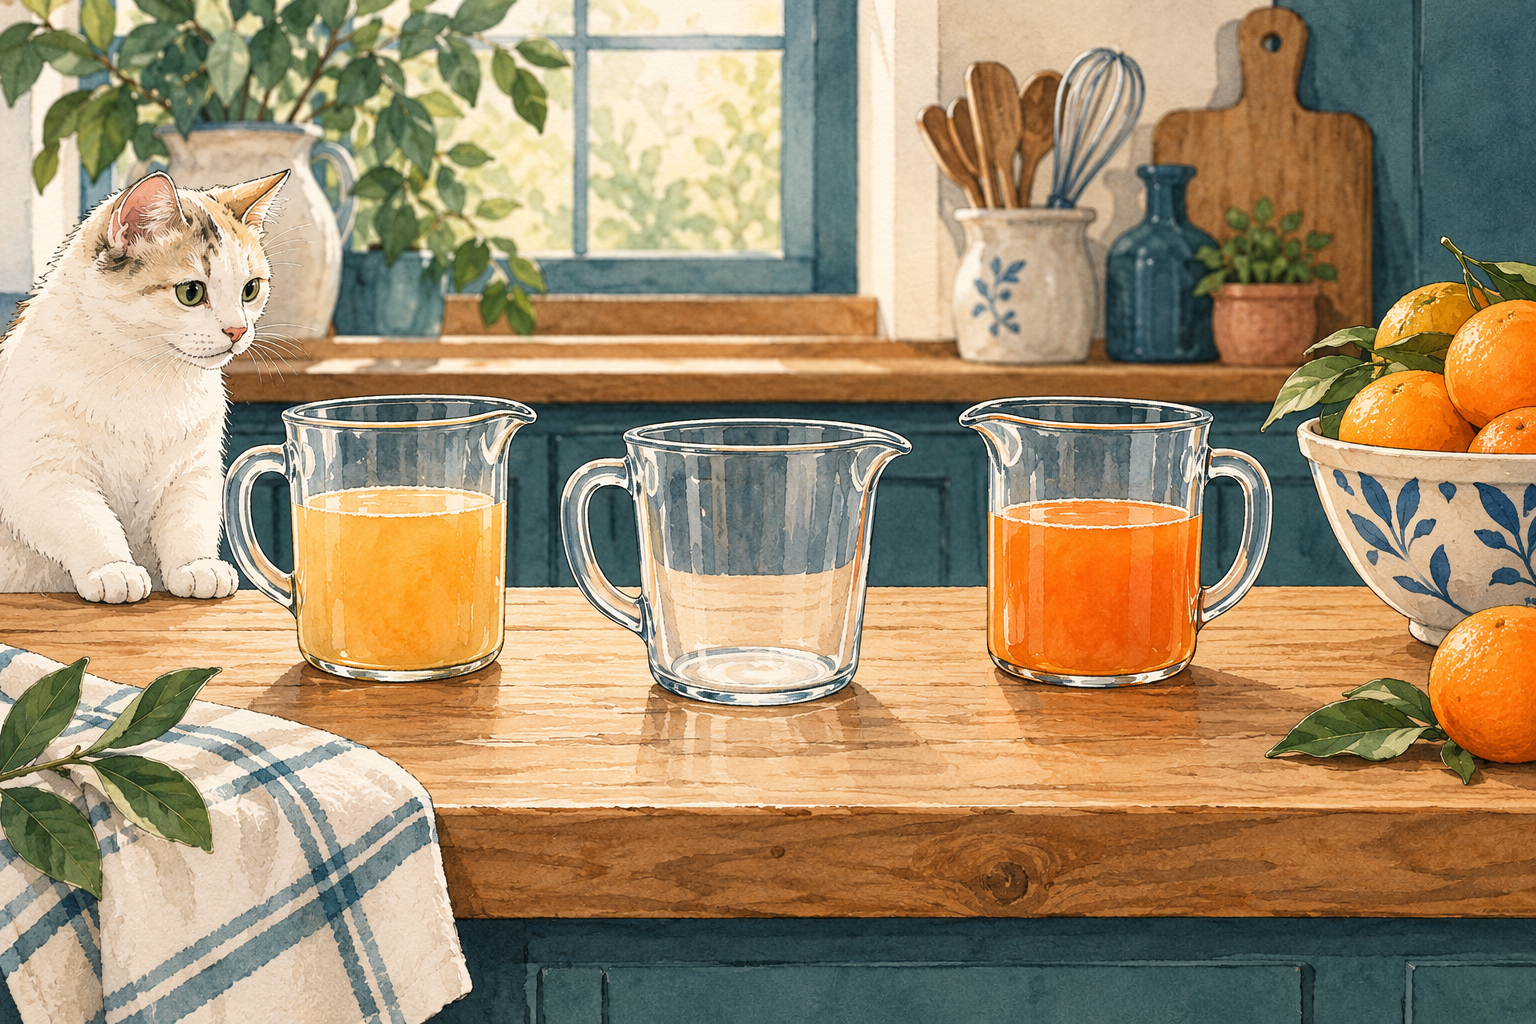
\includegraphics[width=.7\linewidth,height=45mm,keepaspectratio]{images/cats-mixtures.png}\end{center}\par\end{minipage}\par
\noindent\begin{minipage}[t]{\linewidth}\textbf{4.19.} Положительная цена сначала выросла на \(p\%\), затем новая цена выросла на \(q\%\), где \(p,q\ge0\). Докажи, что общее увеличение составляет \(\left(p+q+\dfrac{pq}{100}\right)\%\) от исходной цены.\par\end{minipage}\par
\noindent\begin{minipage}[t]{\linewidth}\textbf{4.20.}\starmark{} Пусть \(\dfrac pq\) --- положительная несократимая дробь с целыми \(p,q>0\). Докажи, что она имеет конечную десятичную запись тогда и только тогда, когда \(q=2^{\alpha}5^{\beta}\) для некоторых \(\alpha,\beta\in\mathbb N_0\). Можно пользоваться основной теоремой арифметики и свойствами делимости.\par\end{minipage}\par
\endgroup

\chapter{Отношения и пропорции}
\begin{definition}\term{Отношение} (\emph{ratio}) \(a\) к \(b\) — частное \(\frac{a}{b}\) при \(b \ne  0\); обозначается \(a : b\).\end{definition}
\begin{definition}\term{Пропорция} (\emph{proportion}) — равенство двух отношений: \(\frac{a}{b} = \frac{c}{d}\), где \(b,\allowbreak d \ne  0\).\end{definition}
\begin{definition}\term{Прямая пропорциональность} (\emph{direct proportion}) — зависимость \(y = kx\) с постоянным ненулевым коэффициентом \(k\).\end{definition}
\begin{definition}\term{Обратная пропорциональность} (\emph{inverse proportion}) — зависимость \(y = \frac{k}{x}\) при \(x \ne  0\) с постоянным ненулевым \(k\).\end{definition}
\begin{definition}\term{Масштаб} (\emph{scale}) \(1 : N\) — отношение длины на карте к длине на местности в одинаковых единицах.\end{definition}
\section*{Основное свойство пропорции}
При \(b,\allowbreak d \ne  0\) равенство \(\frac{a}{b} = \frac{c}{d}\) равносильно \(a \cdot  d = b \cdot  c\).\par
\section*{Правила применения}
При прямой пропорциональности увеличение \(x\) в несколько раз увеличивает \(y\) во столько же раз.\par
При обратной пропорциональности положительных величин увеличение \(x\) в несколько раз уменьшает \(y\) во столько же раз.\par
Деление \(S\) в отношении \(m : n\) при \(m,\allowbreak n > 0\): части равны \(S \cdot  \frac{m}{m + n}\) и \(S \cdot  \frac{n}{m + n}\).\par
{\small\textit{Пример: \(60\) разделить в отношении \(2 : 3\) — это \(24\) и \(36\), поскольку одна часть равна \(\frac{60}{5} = 12\).}}\par
\Needspace{7\baselineskip}\section*{Задачи}
\begin{enumerate}[label={},leftmargin=3.2em,itemsep=10pt]
\Needspace{3\baselineskip}\item[\textbf{5.1.}] Сократи отношение \(18 : 24\).
\Needspace{3\baselineskip}\item[\textbf{5.2.}] Реши пропорцию \(\frac{x}{15} = \frac{4}{5}\).
\Needspace{3\baselineskip}\item[\textbf{5.3.}] Реши пропорцию \(\frac{7}{x} = \frac{21}{18}\).
\Needspace{3\baselineskip}\item[\textbf{5.4.}] Раздели \(64\) в отношении \(3 : 5\).
\Needspace{3\baselineskip}\item[\textbf{5.5.}] Для \(4\) порций нужно \(300\) г крупы. Сколько нужно для \(10\) порций?
\Needspace{3\baselineskip}\item[\textbf{5.6.}] \(5\) одинаковых тетрадей стоят \(180\) рублей. Сколько стоят \(8\)?
\Needspace{3\baselineskip}\item[\textbf{5.7.}] На карте масштаба \(1 : 100 000\) расстояние \(3,5\) см. Найди расстояние на местности в километрах.
\Needspace{3\baselineskip}\item[\textbf{5.8.}] \(6\) рабочих выполняют работу за \(10\) дней. За сколько дней справятся \(15\) рабочих при той же производительности?
\Needspace{3\baselineskip}\item[\textbf{5.9.}] Поездка при скорости \(60\) км/ч занимает \(3\) часа. Сколько займёт при \(90\) км/ч на том же пути?
\Needspace{3\baselineskip}\item[\textbf{5.10.}] Смешивают сок и воду в отношении \(2 : 3\). Сколько каждого компонента нужно для \(1,5\) л смеси?
\Needspace{3\baselineskip}\item[\textbf{5.11.}] При \(y = 3 x\) найди \(y\) для \(x = 4\). Как изменится \(y\) при удвоении \(x\)?
\Needspace{3\baselineskip}\item[\textbf{5.12.}] При \(y = \frac{24}{x}\) найди \(y\) для \(x = 6\). Как изменится \(y\) при удвоении положительного \(x\)?
\Needspace{3\baselineskip}\item[\textbf{5.13.}] Из жизни. Для \(6\) порций супа нужно \(450\) г картофеля. Сколько нужно для \(10\) таких же порций?
\Needspace{3\baselineskip}\item[\textbf{5.14.}] Из жизни. \(4\) одинаковых насоса заполняют бассейн за \(9\) часов. За сколько часов его заполнят \(6\) таких насосов, работающих одновременно?
\Needspace{3\baselineskip}\item[\textbf{5.15.}] Из жизни. Для напитка сироп смешивают с водой в отношении \(1 : 7\). Сколько сиропа и воды нужно для \(2\) л напитка?
\Needspace{3\baselineskip}\item[\textbf{5.16.}\starmark] Рабочие одинаковой производительности: \(6\) человек выполняют работу за \(8\) дней по \(5\) часов. За сколько дней справятся \(4\) человека по \(6\) часов?
\Needspace{3\baselineskip}\item[\textbf{5.17.}\starmark] В смеси отношение сиропа к воде \(2 : 5\). После добавления \(3\) л воды стало \(1 : 4\). Сколько литров смеси было сначала?
\Needspace{3\baselineskip}\item[\textbf{5.18.}\starmark] Автомобиль ехал одинаковое время со скоростями \(60\) и \(90\) км/ч. Найди среднюю скорость. А если одинаковыми были расстояния?
\Needspace{3\baselineskip}\item[\textbf{5.19.}] Пусть \(b,d>0\) и \(\frac ab=\frac cd=k\). Докажи, что \(\frac{a+c}{b+d}=k\).
\Needspace{3\baselineskip}\item[\textbf{5.20.}\starmark] Пусть \(a,b,c,d>0\) и \(\frac ab<\frac cd\). Докажи, что \(\frac ab<\frac{a+c}{b+d}<\frac cd\).
\end{enumerate}

\chapter{Степени с целым показателем}\markright{Глава 6}
\begin{definition}\term{Степень} (\emph{power}) \(a^{n}\) при натуральном \(n\) — произведение \(n\) одинаковых множителей \(a\).\end{definition}
\begin{definition}\term{Основание степени} (\emph{base}) \(a^{n}\) — число \(a\), которое возводят в степень.\end{definition}
\begin{definition}\term{Показатель степени} (\emph{exponent}) \(a^{n}\) — число \(n\); при натуральном \(n\) оно указывает количество одинаковых множителей \(a\).\end{definition}
\begin{definition}\term{Нулевая степень} (\emph{zeroth power}) ненулевого числа определяется равенством \(a^{0} = 1\).\end{definition}
\begin{definition}\term{Отрицательная целая степень} (\emph{negative integer power}) определяется равенством \(a^{- n} = \frac{1}{a^{n}}\) при \(a \ne  0\) и натуральном \(n\).\end{definition}
\begin{definition}\term{Стандартный вид положительного числа} (\emph{scientific notation}) — \(c \cdot  10^{n}\), где \(1 \le  c < 10\) и \(n\) — целое число.\end{definition}
\section*{Свойства степеней}
При умножении степеней одного основания показатели складывают: \(a^{m} \cdot  a^{n} = a^{m + n}\).\par
При делении показатели вычитают: \(\frac{a^{m}}{a^{n}} = a^{m - n},\allowbreak a \ne  0\).\par
При возведении степени в степень показатели перемножают: \((a^{m})^{n} = a^{mn}\).\par
Степень произведения: \((ab)^{n} = a^{n} b^{n}\). Степень дроби: \((\frac{a}{b})^{n} = \frac{a^{n}}{b^{n}},\allowbreak b \ne  0\).\par
Эти правила для целых показателей применяют только там, где все выражения определены; отрицательные степени требуют ненулевых оснований.\par
{\small\textit{Пример: \((- 2)^{4} = 16\), но \(- 2^{4} = - 16\). Число \(0,0032\) в стандартном виде: \(3{,}2 \cdot  10^{- 3}\).}}\par

\Needspace{7\baselineskip}\section*{Задачи}
\begingroup\setlength{\parskip}{3pt}
\noindent\begin{minipage}[t]{\linewidth}\textbf{6.1.} Вычисли \(2^{5}\).\par\end{minipage}\par
\noindent\begin{minipage}[t]{\linewidth}\textbf{6.2.} Вычисли \((- 3)^{4}\) и \(- 3^{4}\).\par\end{minipage}\par
\noindent\begin{minipage}[t]{\linewidth}\textbf{6.3.} Вычисли \(7^{0} + 2^{- 3}\).\par\end{minipage}\par
\noindent\begin{minipage}[t]{\linewidth}\textbf{6.4.} Представь одной степенью: \(5^{3} \cdot  5^{4}\).\par\end{minipage}\par
\noindent\begin{minipage}[t]{\linewidth}\textbf{6.5.} Представь одной степенью: \(2^{9} : 2^{4}\).\par\end{minipage}\par
\noindent\begin{minipage}[t]{\linewidth}\textbf{6.6.} Представь одной степенью: \((3^{2})^{4}\).\par\end{minipage}\par
\par\addvspace{5pt}\begin{lrbox}{\CatFlowBox}\begin{minipage}[t]{\linewidth}
\setlength{\parskip}{5pt}\setlength{\columnsep}{4.5mm}\setlength{\intextsep}{0pt}
\begin{wrapfigure}[13]{l}{54mm}
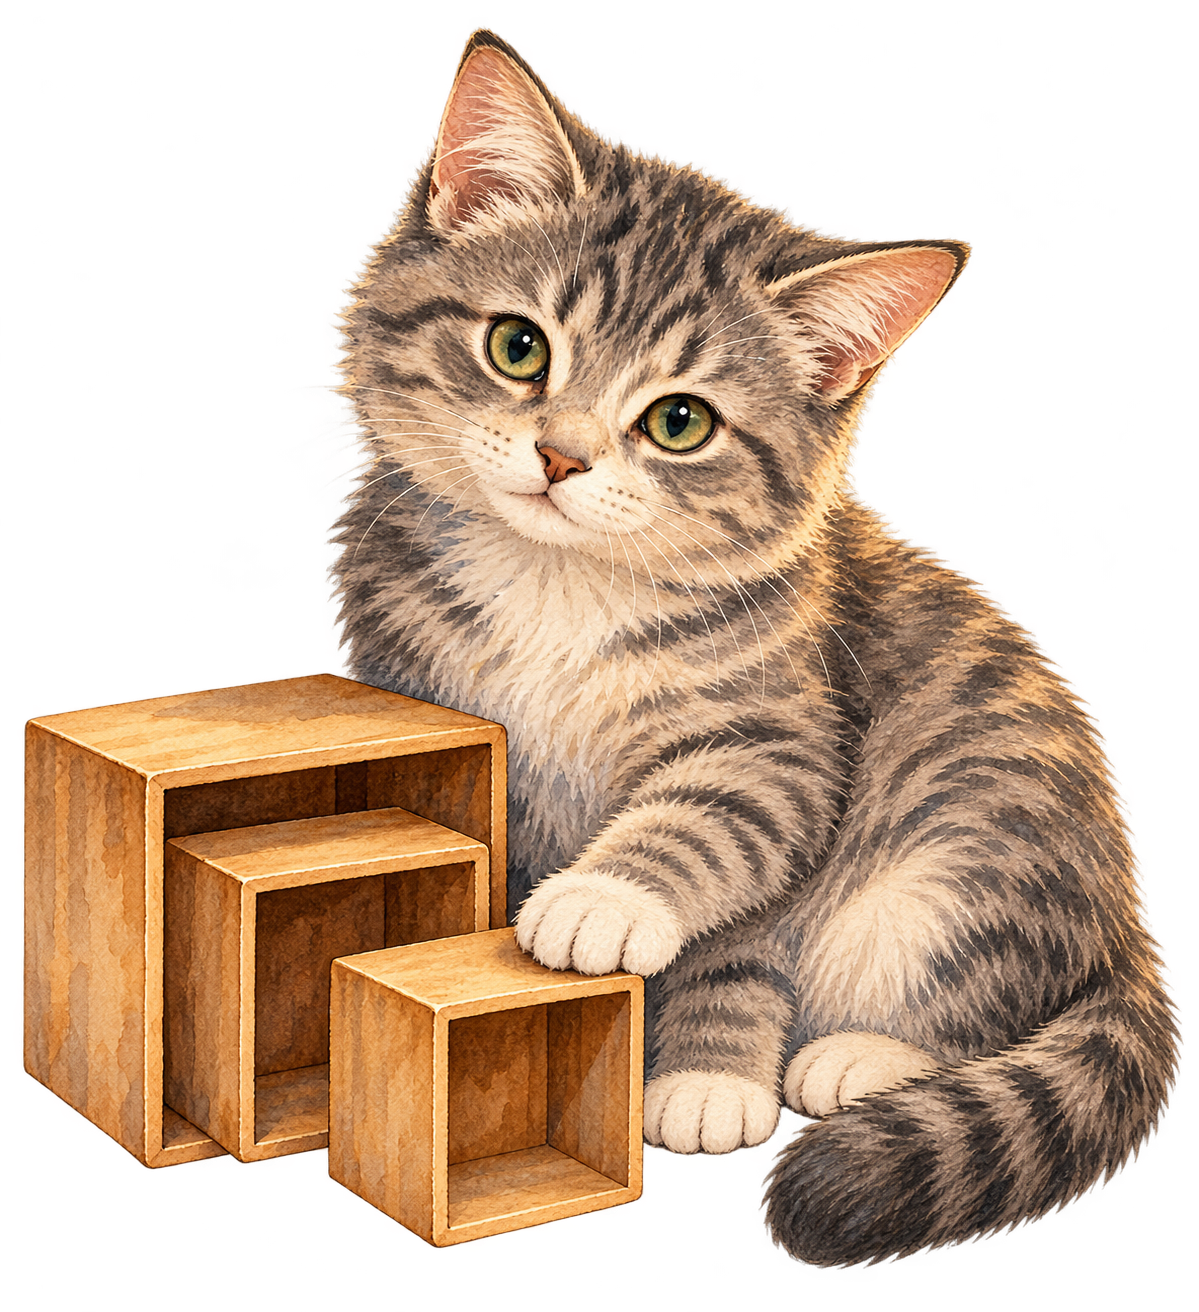
\includegraphics[width=54mm,height=58mm,keepaspectratio]{images/unique/art-11.png}
\end{wrapfigure}
\textbf{6.7.} Вычисли \((\dfrac{2}{3})^{- 2}\).\par

\textbf{6.8.} Вычисли \(10^{- 3} \cdot  10^{5}\).\par

\textbf{6.9.} Запиши \(0{,}00056\) в стандартном виде.\par

\textbf{6.10.} Запиши \(7{,}2 \cdot  10^{5}\) обычным числом.\par

\textbf{6.11.} Упрости \(a^{5} \cdot  a^{- 2}\) при \(a \ne  0\).\par

\textbf{6.12.} Вычисли \((- 2)^{3} \cdot  2^{- 2} + 3^{0}\).\par

\textbf{6.13.} Из жизни. В модели опыта каждая бактерия делится на две раз в час. Вначале была одна бактерия. Сколько их станет через \(8\) часов?\par
\par\WFclear\end{minipage}\end{lrbox}%
\ifdim\dimexpr\ht\CatFlowBox+\dp\CatFlowBox\relax<64mm\dp\CatFlowBox=\dimexpr64mm-\ht\CatFlowBox\relax\fi%
\noindent\usebox{\CatFlowBox}\par\addvspace{5pt}

\noindent\begin{minipage}[t]{\linewidth}\textbf{6.14.} Из жизни. Квадратный участок имеет сторону \(10^{3}\) м. Запиши его площадь степенью десяти и обычным числом в м\(^{2}\).\par\end{minipage}\par
\noindent\begin{minipage}[t]{\linewidth}\textbf{6.15.} Из жизни. В одном файле \(4 \cdot  10^{6}\) байт. Сколько байт в \(3 \cdot  10^{2}\) таких файлах?\par\end{minipage}\par
\noindent\begin{minipage}[t]{\linewidth}\textbf{6.16.}\starmark{} Вычисли: \(\dfrac{2^{- 3} \cdot  4^{2}}{8^{- 1}}\).\par\end{minipage}\par
\noindent\begin{minipage}[t]{\linewidth}\textbf{6.17.}\starmark{} Вычисли: \(\dfrac{3^{5} - 3^{4}}{3^{3} + 3^{2}}\).\par\end{minipage}\par
\noindent\begin{minipage}[t]{\linewidth}\textbf{6.18.}\starmark{} В модели файл каждый день увеличивается втрое. Через \(4\) дня его размер \(162\) МБ. Каков был размер сначала и каким станет через \(6\) дней от начала?\par\end{minipage}\par
\noindent\begin{minipage}[t]{\linewidth}\textbf{6.19.} Докажите, что \(a^m a^n=a^{m+n}\) для действительного \(a\) и натуральных \(m,n\), непосредственно используя определение натуральной степени.\par\end{minipage}\par
\noindent\begin{minipage}[t]{\linewidth}\textbf{6.20.} Пусть \(a\neq0\), \(m,n\) — натуральные числа. Докажите \(a^{-m}a^{-n}=a^{-(m+n)}\), используя определение отрицательной степени.\par\end{minipage}\par
\endgroup

\chapter{Корни и действительные числа}\markright{Глава 7}
\begin{definition}\term{Арифметический квадратный корень} (\emph{principal square root}) \(\sqrt{a}\) — неотрицательное число, квадрат которого равен \(a\). В действительных числах определён при \(a \ge  0\). При \(a>0\) уравнение \(z^2=a\) имеет два корня: \(z=\sqrt a\) и \(z=-\sqrt a\).\end{definition}
\begin{definition}\term{Кубический корень} (\emph{cube root}) \(\sqrt[3]{a}\) — число, куб которого равен \(a\); существует для любого действительного \(a\).\end{definition}
\begin{definition}\term{Рациональное число} (\emph{rational number}) — число вида \(\frac{p}{q}\), где \(p,\allowbreak q\) — целые и \(q \ne  0\).\end{definition}
\begin{definition}\term{Иррациональное число} (\emph{irrational number}) — действительное число, которое нельзя представить в виде \(\frac{p}{q}\) с целыми \(p,q\) и \(q\ne0\).\end{definition}
\section*{Свойства корней}
При \(a,\allowbreak b \ge 0\): \(\sqrt{ab} = \sqrt{a} \cdot \sqrt{b}\).\par
При \(a \ge 0,\allowbreak b > 0\): \(\sqrt{\frac{a}{b}} = \frac{\sqrt{a}}{\sqrt{b}}\).\par
Для любого действительного \(x\): \(\sqrt{x^{2}} = | x |\).\par
Для \(a,\allowbreak b \ge  0\) из \(a < b\) следует \(\sqrt{a} < \sqrt{b}\).\par
{\small\textit{Примеры: \(\sqrt{72} = \sqrt{36 \cdot  2} = 6 \sqrt{2};\allowbreak \sqrt{(- 5)^{2}} = 5;\allowbreak \sqrt[3]{- 8} = - 2\).}}\par
\section*{Теорема Пифагора}
\begin{theorem}[Пифагор; Pythagorean theorem]
В прямоугольном треугольнике с катетами \(a,b\) и гипотенузой \(c\) выполнено \(a^2+b^2=c^2\).
\end{theorem}
\begin{proof}Расположим четыре таких треугольника внутри квадрата со стороной \(a+b\) так, чтобы их гипотенузы ограничивали внутренний квадрат со стороной \(c\). Сравнение площадей даёт \((a+b)^2=4\frac{ab}{2}+c^2\). После раскрытия скобок получаем требуемое равенство.\end{proof}
\subsection*{Корень произвольной натуральной степени}
\begin{definition}
\term{Корень нечётной степени} (odd-index root) \(n\geq 3\) из действительного числа \(a\) — единственное действительное число \(x\), для которого \(x^n=a\). Обозначение: \(x=\sqrt[n]{a}\).
\end{definition}
\begin{definition}
\term{Арифметический корень чётной степени} (principal even-index root) \(n\geq2\) из числа \(a\geq0\) — единственное \emph{неотрицательное} число \(x\), для которого \(x^n=a\). Обозначение: \(x=\sqrt[n]{a}\). При \(a<0\) такой действительный корень не определён.
\end{definition}
В общей записи \(\sqrt[n]{a}\) термин \term{корень \(n\)-й степени} (\(n\)th root) относится к одному из этих двух случаев. Здесь \(n\) — натуральное число, \(n\geq2\). Квадратный корень \(\sqrt a\) — это \(\sqrt[2]a\).

Не путайте значение корня с решениями уравнения: \(\sqrt[4]{16}=2\), а уравнение \(x^4=16\) имеет два действительных решения \(x=2\) и \(x=-2\). При нечётном \(n\) знак \(\sqrt[n]a\) совпадает со знаком \(a\).

\begin{theorem}[Корень из степени]
Для любого действительного \(x\) и натурального \(n\geq2\)
\[
\sqrt[n]{x^n}=
\begin{cases}
 x,&n\text{ нечётно},\\
 |x|,&n\text{ чётно}.
\end{cases}
\]
\end{theorem}
\begin{proof}
При нечётном \(n\) число \(x\) само является действительным корнем уравнения \(y^n=x^n\). При чётном \(n\) число \(|x|\) неотрицательно и \(|x|^n=x^n\), поэтому оно и является арифметическим корнем. Единственность в определении даёт оба равенства.
\end{proof}

\begin{theorem}[Произведение и частное корней]
Если \(n\geq2\) нечётно, то для любых действительных \(a,b\)
\[
\sqrt[n]{ab}=\sqrt[n]a\,\sqrt[n]b.
\]
Если \(n\) чётно, это равенство верно при \(a\geq0\) и \(b\geq0\). Для частного дополнительно требуется \(b\neq0\):
\[
\sqrt[n]{\frac ab}=\frac{\sqrt[n]a}{\sqrt[n]b}.
\]
Таким образом, при чётном \(n\) условия для частного: \(a\geq0\), \(b>0\); при нечётном: \(a\in\mathbb R\), \(b\in\mathbb R\setminus\{0\}\).
\end{theorem}
\par\addvspace{5pt}\begin{lrbox}{\CatFlowBox}\begin{minipage}[t]{\linewidth}
\setlength{\parskip}{5pt}\setlength{\columnsep}{4.5mm}\setlength{\intextsep}{0pt}
\begin{wrapfigure}[13]{r}{54mm}

\includegraphics[width=54mm,height=58mm,keepaspectratio]{images/unique/art-12.png}
\end{wrapfigure}
\textit{Доказательство.} Пусть \(u=\sqrt[n]a\), \(v=\sqrt[n]b\). Тогда \((uv)^n=u^nv^n=ab\). При чётном \(n\) дополнительно \(uv\geq0\), поэтому \(uv\) — именно арифметический корень. Для частного \(v\neq0\) и \((\frac uv)^n=\frac ab\); при чётном \(n\) имеем \(\frac uv\geq0\). Снова применяем единственность корня.\hfill\(\square\)
\par\WFclear\end{minipage}\end{lrbox}%
\ifdim\dimexpr\ht\CatFlowBox+\dp\CatFlowBox\relax<64mm\dp\CatFlowBox=\dimexpr64mm-\ht\CatFlowBox\relax\fi%
\noindent\usebox{\CatFlowBox}\par\addvspace{5pt}


\begin{theorem}[Корень из корня]
Для натуральных \(m,n\geq2\) и \(a\geq0\)
\[
\sqrt[m]{\sqrt[n]a}=\sqrt[mn]a.
\]
Если \(m\) и \(n\) оба нечётны, равенство справедливо также при \(a<0\).
\end{theorem}
\begin{proof}
Обозначим левую часть через \(u\). Тогда \(u^m=\sqrt[n]a\), откуда \(u^{mn}=a\). При \(a\geq0\) число \(u\) неотрицательно; при отрицательном \(a\) и нечётных \(m,n\) степень \(mn\) нечётна. В каждом из указанных случаев \(u\) является корнем, определённым в правой части.
\end{proof}

\begin{example}
\(\sqrt[4]{80}=\sqrt[4]{16\cdot5}=2\sqrt[4]5\),
\(\sqrt[3]{-81}=-3\sqrt[3]3\),
\(\sqrt[6]{(-2)^6}=2\),
\(\sqrt[5]{(-2)^5}=-2\).
\end{example}

\subsection*{Рациональный показатель степени}
\begin{definition}
Пусть \(a>0\), \(m\in\mathbb Z\), \(n\in\mathbb N\). \term{Степень с рациональным показателем} (rational exponent) определяется равенством
\[
a^{\frac mn}=\bigl(\sqrt[n]a\bigr)^m.
\]
При \(n=1\) здесь имеется в виду обычная целая степень, а не новый корень. Отрицательный показатель означает обратную величину: \(a^{-\frac mn}=\frac{1}{a^{\frac mn}}\).
\end{definition}

\begin{theorem}[Независимость от записи дроби]
Для \(a>0\) значение \(a^{\frac mn}\) зависит только от рационального числа \(\frac mn\), а не от выбранных числителя и знаменателя.
\end{theorem}
\begin{proof}
Если \(\frac mn=\frac pq\), где \(n,q>0\), то \(mq=pn\). Оба числа \((\sqrt[n]a)^m\) и \((\sqrt[q]a)^p\) положительны. После возведения в натуральную степень \(nq\) они дают соответственно \(a^{mq}\) и \(a^{pn}\), то есть одинаковые числа. Два положительных числа с одинаковыми натуральными степенями равны. Последний факт следует из строгого возрастания натуральной степени на положительной полуоси: при \(0<u<v\) имеем \(u^N<v^N\).
\end{proof}

\begin{theorem}[Свойства рациональных степеней]
Пусть \(a,b>0\), \(r,s\in\mathbb Q\). Тогда
\[
\begin{aligned}
a^r a^s&=a^{r+s},&\qquad \frac{a^r}{a^s}&=a^{r-s},\\
(a^r)^s&=a^{rs},&(ab)^r&=a^rb^r,\\
\left(\frac ab\right)^r&=\frac{a^r}{b^r}.
\end{aligned}
\]
\end{theorem}
\begin{proof}
Приведём \(r=\frac mn\), \(s=\frac pn\) к общему положительному знаменателю и положим \(u=\sqrt[n]a>0\). Тогда \(a^ra^s=u^mu^p=u^{m+p}\); для частного рассуждение такое же. Для правила степени степени пусть \(r=\frac mn\), \(s=\frac pq\). Числа \((a^r)^s\) и \(a^{rs}\) положительны; их степени \(nq\) обе равны \(a^{mp}\), поэтому эти числа равны. Наконец, из свойства корня произведения получаем \((ab)^{\frac mn}=(\sqrt[n]a\sqrt[n]b)^m=a^{\frac mn}b^{\frac mn}\); для частного аналогично. Целые отрицательные показатели допускаются, поскольку все основания и корни ненулевые.
\end{proof}

\section*{Нулевое и отрицательное основания}
Для \(r>0\) принимают \(0^r=0\). Записи \(0^0\) и \(0^r\) при \(r<0\) в этом сборнике не определены.

Для \(a<0\) используем следующую договорённость: сначала записываем рациональное число \(r=\frac mn\) как \term{несократимую дробь} (reduced fraction), где \(n>0\). Действительную степень \(a^{\frac mn}\) определяем только при нечётном \(n\):
\[
a^{\frac mn}=\bigl(\sqrt[n]a\bigr)^m.
\]
При чётном знаменателе несократимой дроби такая действительная степень не определена. Например,
\[
(-243)^{\frac25}=9,\qquad
(-27)^{-\frac13}=-\frac13,\qquad
(-4)^{\frac12}\text{ не определена в }\mathbb R.
\]
Общими правилами степеней для отрицательных оснований пользоваться без проверки нельзя. Например,
\[
\bigl((-1)^2\bigr)^{\frac12}=1,
\qquad
(-1)^{2\cdot(\frac12)}=-1.
\]
Также \((-8)^{\frac26}=(-8)^{\frac13}=-2\), тогда как \(\sqrt[6]{(-8)^2}=2\). Условие \(a>0\) в теореме о свойствах рациональных степеней существенно.

\par\noindent\begin{minipage}{\linewidth}\section*{Графики}
\begin{center}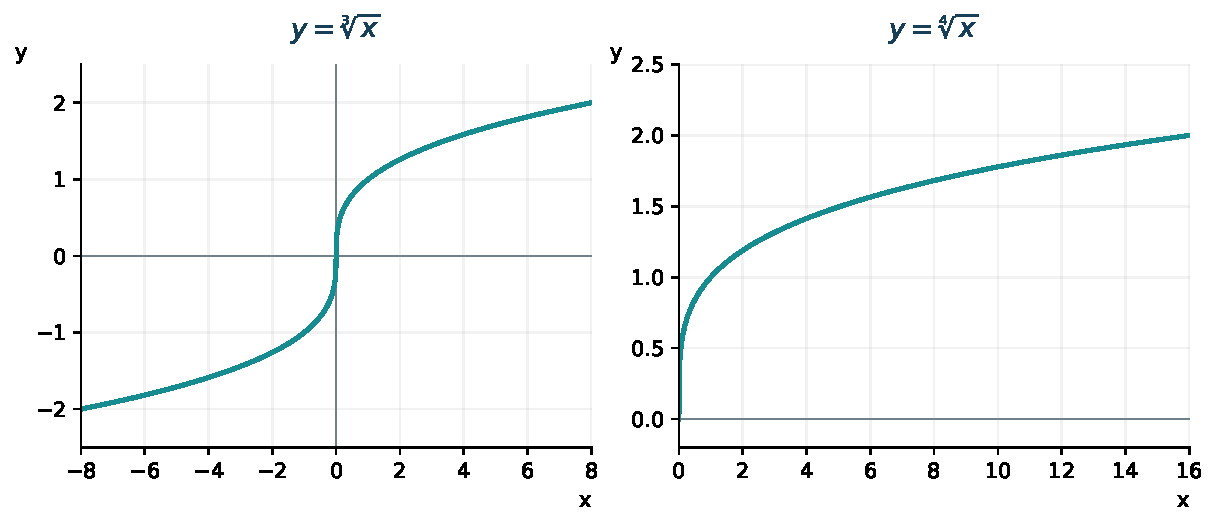
\includegraphics[width=\textwidth,height=.79\textheight,keepaspectratio]{images/atlas-roots.pdf}\par\small Корни нечётной и чётной степени\end{center}\end{minipage}\par
\Needspace{7\baselineskip}\section*{Задачи}
\begingroup\setlength{\parskip}{3pt}
\noindent\begin{minipage}[t]{\linewidth}\textbf{7.1.} Вычисли \(\sqrt{81}\) и \(\sqrt[3]{- 27}\).\par\end{minipage}\par
\noindent\begin{minipage}[t]{\linewidth}\textbf{7.2.} Вычисли \(\sqrt{\dfrac{49}{100}}\).\par\end{minipage}\par
\noindent\begin{minipage}[t]{\linewidth}\textbf{7.3.} Упрости \(\sqrt{72}\).\par\end{minipage}\par
\noindent\begin{minipage}[t]{\linewidth}\textbf{7.4.} Упрости \(\sqrt{200} - \sqrt{50}\).\par\end{minipage}\par
\par\addvspace{5pt}\begin{lrbox}{\CatFlowBox}\begin{minipage}[t]{\linewidth}
\setlength{\parskip}{5pt}\setlength{\columnsep}{4.5mm}\setlength{\intextsep}{0pt}
\begin{wrapfigure}[12]{r}{54mm}
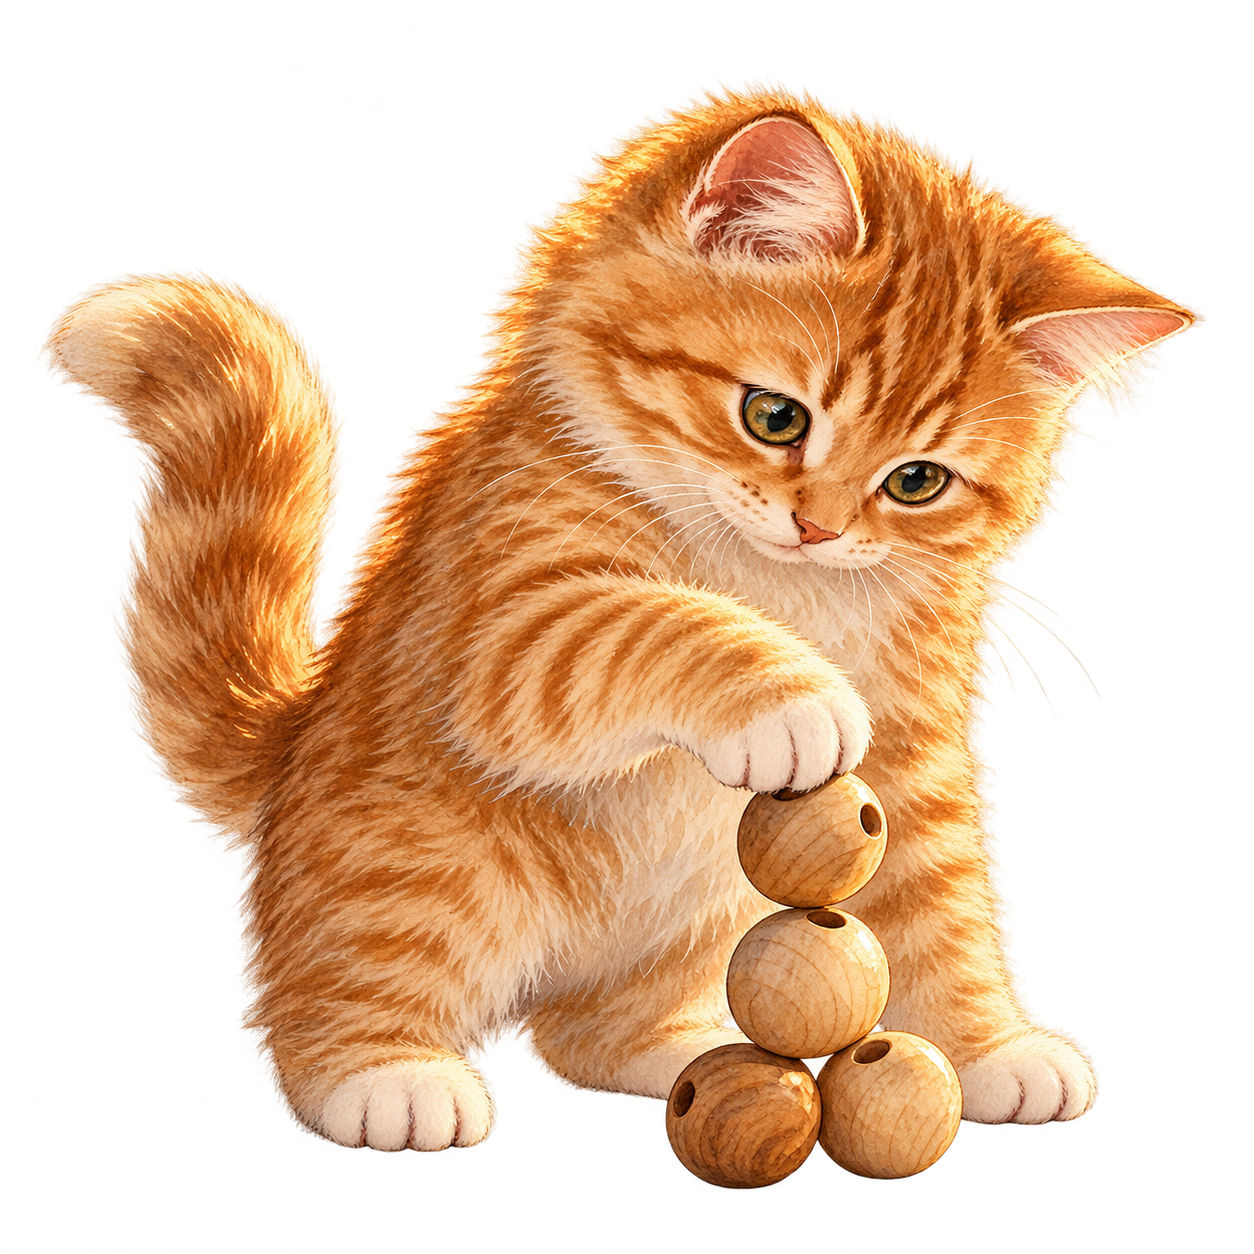
\includegraphics[width=54mm,height=58mm,keepaspectratio]{images/unique/art-22.png}
\end{wrapfigure}
\textbf{7.5.} Внеси множитель под корень: \(3 \sqrt{5}\).\par

\textbf{7.6.} Вычисли \(\sqrt{12} \cdot  \sqrt{3}\).\par

\textbf{7.7.} Вычисли \(\dfrac{\sqrt{75}}{\sqrt{3}}\).\par

\textbf{7.8.} Вычисли \(\sqrt{(- 7)^{2}}\).\par

\textbf{7.9.} Между какими соседними целыми числами находится \(\sqrt{30}\)?\par

\textbf{7.10.} Сравни \(\sqrt{7}\) и \(2{,}7\).\par

\textbf{7.11.} Какие числа рациональные: \(\sqrt{16},\allowbreak \sqrt{2},\allowbreak - \dfrac{3}{7},\allowbreak 0{,}(3),\allowbreak \pi \)?\par
\par\WFclear\end{minipage}\end{lrbox}%
\ifdim\dimexpr\ht\CatFlowBox+\dp\CatFlowBox\relax<64mm\dp\CatFlowBox=\dimexpr64mm-\ht\CatFlowBox\relax\fi%
\noindent\usebox{\CatFlowBox}\par\addvspace{5pt}

\noindent\begin{minipage}[t]{\linewidth}\textbf{7.12.} Существуют ли \(\sqrt{- 9}\) и \(\sqrt[3]{- 8}\) в действительных числах?\par\end{minipage}\par
\noindent\begin{minipage}[t]{\linewidth}\textbf{7.13.} Квадратная комната имеет площадь \(49\) м\(^{2}\). Найди длину её стороны.\par\end{minipage}\par
\noindent\begin{minipage}[t]{\linewidth}\textbf{7.14.} Лестница стоит у стены: её основание в \(3\) м от стены, верх на высоте \(4\) м. Найди длину лестницы. Считай стену и землю перпендикулярными.\begin{center}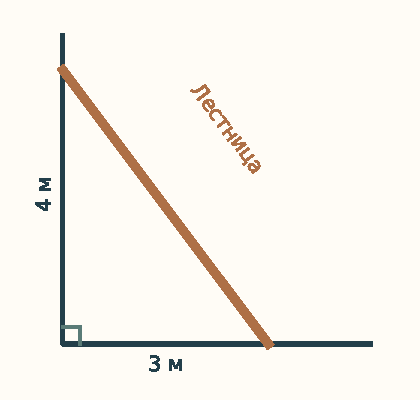
\includegraphics[width=.7\linewidth,height=45mm,keepaspectratio]{images/diagram-ladder.pdf}\end{center}\par\end{minipage}\par
\noindent\begin{minipage}[t]{\linewidth}\textbf{7.15.} У кубического контейнера объём \(0{,}125\) м\(^{3}\). Найди длину ребра в метрах и сантиметрах.\par\end{minipage}\par
\noindent\begin{minipage}[t]{\linewidth}\textbf{7.16.}\starmark{} Упрости: \(\sqrt{48} + \sqrt{75} - \sqrt{147}\).\par\end{minipage}\par
\noindent\begin{minipage}[t]{\linewidth}\textbf{7.17.}\starmark{} Проверь без десятичных приближений утверждение \(\sqrt{2} + \sqrt{3} > \sqrt{10}\). Докажи его или опровергни.\par\end{minipage}\par
\noindent\begin{minipage}[t]{\linewidth}\textbf{7.18.}\starmark{} У прямоугольника площадь \(48\) м\(^{2}\), одна сторона втрое длиннее другой. Найди обе стороны и диагональ.\par\end{minipage}\par
\noindent\begin{minipage}[t]{\linewidth}\textbf{7.19.} Докажите равенство \(\sqrt[n]{x^n}=|x|\) для любого действительного \(x\) и любого чётного натурального \(n\geq2\).\par\end{minipage}\par
\noindent\begin{minipage}[t]{\linewidth}\textbf{7.20.} Докажите, что для нечётного натурального \(n\geq3\) и любого действительного \(a\) выполнено \(\sqrt[n]{-a}=-\sqrt[n]a\).\par\end{minipage}\par
\noindent\begin{minipage}[t]{\linewidth}\textbf{7.21.} Вычислите \(\sqrt[4]{81}\), \(\sqrt[5]{-32}\) и \(\sqrt[6]{64}\).\par\end{minipage}\par
\par\addvspace{5pt}\begin{lrbox}{\CatFlowBox}\begin{minipage}[t]{\linewidth}
\setlength{\parskip}{5pt}\setlength{\columnsep}{4.5mm}\setlength{\intextsep}{0pt}
\begin{wrapfigure}[12]{l}{54mm}
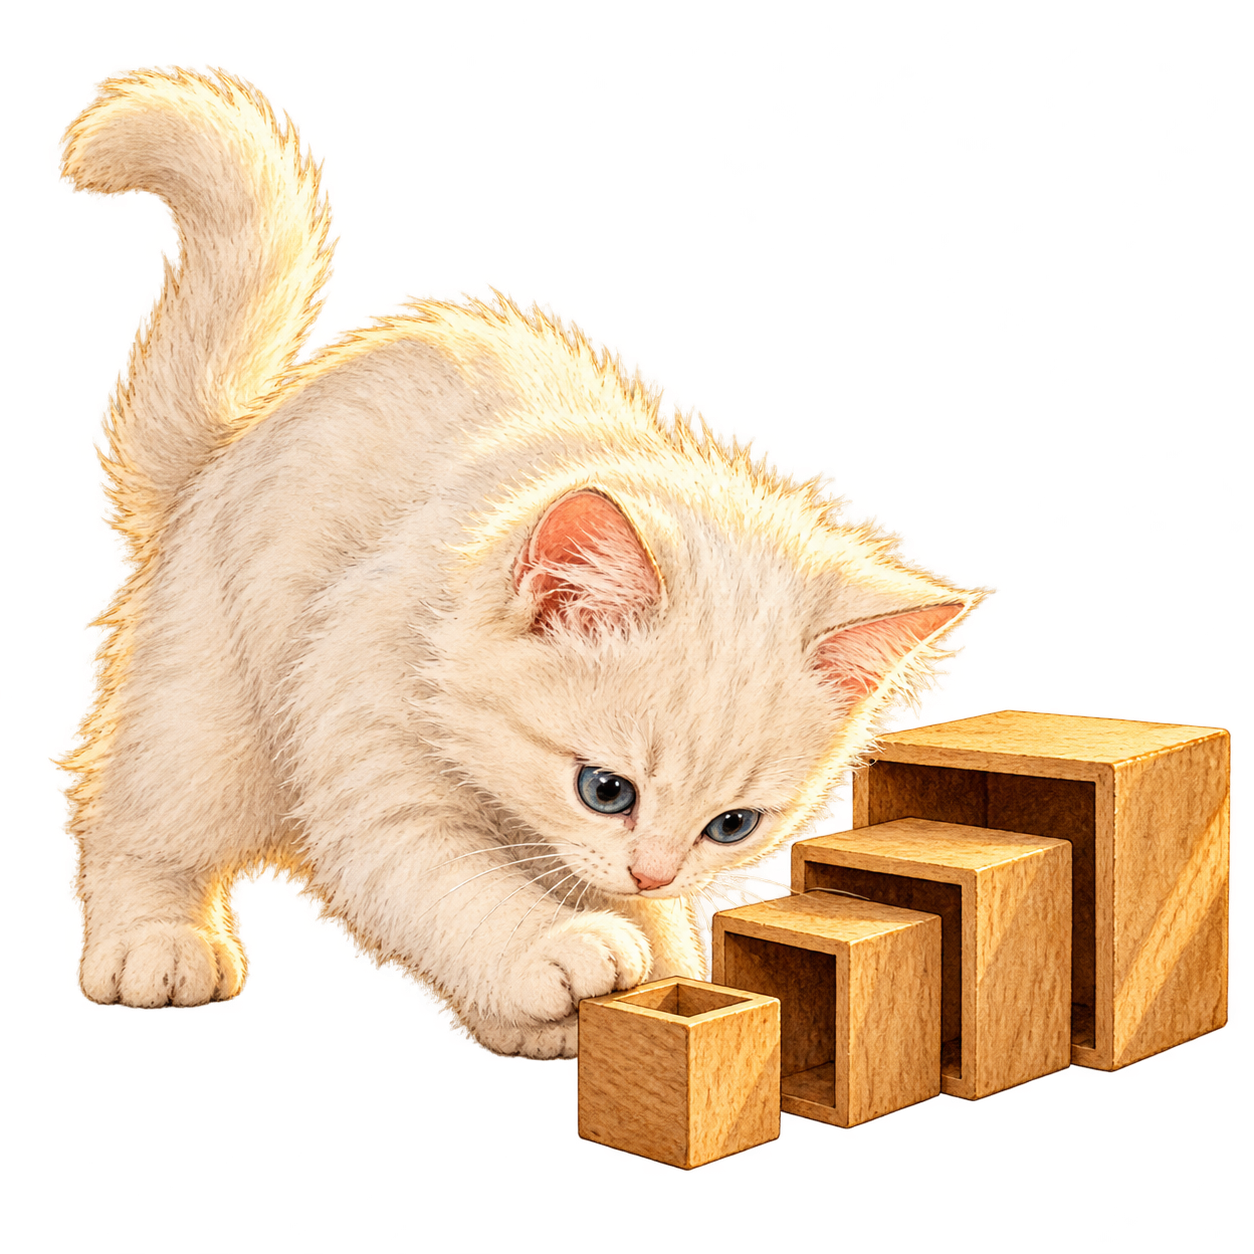
\includegraphics[width=54mm,height=58mm,keepaspectratio]{images/unique/art-15.png}
\end{wrapfigure}
\textbf{7.22.} Какие из выражений \(\sqrt[4]{-16}\), \(\sqrt[3]{-64}\), \(\sqrt[6]{0}\) определены в действительных числах? Вычислите определённые.\par

\textbf{7.23.} Упростите \(\sqrt[6]{x^6}\) и \(\sqrt[5]{x^5}\) для действительного \(x\).\par

\textbf{7.24.} Упростите \(\sqrt[4]{48}\) и вычислите \(\dfrac{\sqrt[3]{54}}{\sqrt[3]2}\).\par

\textbf{7.25.} Вычислите \((-32)^{\dfrac25}\), \((-8)^{-\dfrac13}\) и \(16^{-\dfrac34}\).\par

\textbf{7.26.} Решите в действительных числах \(\sqrt[4]{x+7}=2\) и \(\sqrt[3]{2x-1}=-3\).\par

\textbf{7.27.}\starmark{} Найдите область определения \(f(x)=\dfrac1{\sqrt[4]{x-2}}+\sqrt[3]{x+1}\).\par

\textbf{7.28.}\starmark{} Решите \(\sqrt[4]{(x-1)^4}=2-x\) в действительных числах.\par
\par\WFclear\end{minipage}\end{lrbox}%
\ifdim\dimexpr\ht\CatFlowBox+\dp\CatFlowBox\relax<64mm\dp\CatFlowBox=\dimexpr64mm-\ht\CatFlowBox\relax\fi%
\noindent\usebox{\CatFlowBox}\par\addvspace{5pt}

\endgroup

\chapter{Модуль и числовые промежутки}
\begin{definition}\term{Модуль} (\emph{absolute value}) \(| x |\) — расстояние от числа \(x\) до нуля на числовой прямой: \(| x | = x\) при \(x \ge  0\) и \(| x | = - x\) при \(x < 0\).\end{definition}
\begin{definition}\term{Числовой промежуток} (\emph{interval}) — множество всех чисел между заданными границами с указанным включением или исключением концов.\end{definition}
\begin{definition}\term{Пересечение} (\emph{intersection}) множеств \(A\) и \(B\), обозначаемое \(A\cap B\), — множество элементов, принадлежащих одновременно обоим множествам.\end{definition}
\begin{definition}\term{Объединение} (\emph{union}) множеств \(A\) и \(B\), обозначаемое \(A\cup B\), — множество элементов, принадлежащих хотя бы одному из этих множеств.\end{definition}
\section*{Свойства модуля}
\(| x | \ge  0;\allowbreak | x | = 0\) только при \(x = 0\). Также \(| - x | = | x |\) и \(| ab | = | a | | b |\).\par
Расстояние между числами \(a\) и \(b\) равно \(| a - b |\).\par
Неравенство треугольника: \(| a + b | \le  | a | + | b |\).\par
При \(r > 0\) условие \(| x - a | < r\) означает \(a - r < x < a + r\). При \(r>0\) условие \(|x-a|\le r\) равносильно \(a-r\le x\le a+r\).\par
\section*{Запись промежутков}
\((a;\allowbreak b)\): \(a < x < b\). \([a;\allowbreak b]\): \(a \le x \le b\). \([a;\allowbreak b)\) и \((a;\allowbreak b]\) включают только один из концов.\par
Бесконечные границы всегда записывают с круглой скобкой: например, \((- \infty ;\allowbreak 3]\).\par
{\small\textit{Пример: \(| x - 2 | \le  3\) равносильно \(- 1 \le  x \le  5\), то есть \(x \in  [- 1;\allowbreak 5]\).}}\par

\Needspace{7\baselineskip}\section*{Задачи}
\begin{enumerate}[label={},leftmargin=3.2em,itemsep=10pt]
\Needspace{3\baselineskip}\item[\textbf{8.1.}] Вычисли \(| - 8 | + | 3 |\).
\Needspace{3\baselineskip}\item[\textbf{8.2.}] Вычисли \(| - 5 + 2 |\).
\Needspace{3\baselineskip}\item[\textbf{8.3.}] Найди расстояние между \(- 7\) и \(4\).
\Needspace{3\baselineskip}\item[\textbf{8.4.}] Сравни \(| - 6 |\) и \(| 5 |\).
\Needspace{3\baselineskip}\item[\textbf{8.5.}] Запиши \(- 2 < x \le  3\) промежутком.
\Needspace{3\baselineskip}\item[\textbf{8.6.}] Запиши \([- 4;\allowbreak 1)\) двойным неравенством.
\Needspace{3\baselineskip}\item[\textbf{8.7.}] Выпиши целые числа из \((- 3;\allowbreak 2]\).
\Needspace{3\baselineskip}\item[\textbf{8.8.}] Найди пересечение \([- 2;\allowbreak 4]\) и \((1;\allowbreak 7)\).
\Needspace{3\baselineskip}\item[\textbf{8.9.}] Найди объединение \((- \infty ;\allowbreak 2]\) и \((1;\allowbreak 5)\).
\Needspace{3\baselineskip}\item[\textbf{8.10.}] Реши \(| x | = 5\).
\Needspace{3\baselineskip}\item[\textbf{8.11.}] Реши \(| x - 2 | < 3\).
\Needspace{3\baselineskip}\item[\textbf{8.12.}] Упрости \(\sqrt{x^{2}}\) и вычисли при \(x = - 4\).
\Needspace{3\baselineskip}\item[\textbf{8.13.}] Из жизни. Температура в морозилке \(- 18 {}^{\circ} C\), а в комнате \(+ 22 {}^{\circ} C\). На сколько градусов отличаются температуры?
\Needspace{3\baselineskip}\item[\textbf{8.14.}] Из жизни. Длина детали должна отличаться от \(50\) мм не более чем на \(0,2\) мм. Запиши допустимые длины \(x\) через модуль и промежутком.
\Needspace{3\baselineskip}\item[\textbf{8.15.}] Из жизни. Аттракцион доступен при росте от \(120\) см включительно до \(190\) см не включительно. Запиши условие для роста \(h\) неравенством и промежутком. Можно ли войти при росте \(190\) см?
\Needspace{3\baselineskip}\item[\textbf{8.16.}\starmark] Реши \(| x - 3 | + | x + 1 | = 6\).
\Needspace{3\baselineskip}\item[\textbf{8.17.}\starmark] Найди все целые \(x\), для которых \(| 2 x - 1 | \le  5\) и \(x \notin  [0;\allowbreak 2)\).
\Needspace{3\baselineskip}\item[\textbf{8.18.}\starmark] Два датчика допускают температуру: первый \(| t - 20 | \le  3\), второй \(| t - 24 | < 4\). Найди общий допустимый диапазон.
\Needspace{3\baselineskip}\item[\textbf{8.19.}] Докажите обратное неравенство треугольника \(\bigl||a|-|b|\bigr|\leq|a-b|\) для действительных \(a,b\).
\Needspace{3\baselineskip}\item[\textbf{8.20.}] Докажите, что при \(r>0\) неравенство \(|x-a|\leq r\) равносильно \(a-r\leq x\leq a+r\).
\end{enumerate}

\chapter{Преобразование алгебраических выражений}
\begin{definition}\term{Подобные слагаемые} (\emph{like terms}) — слагаемые с одинаковой буквенной частью, включая показатели степеней.\end{definition}
\begin{definition}\term{Разложение на множители} (\emph{factorization}) — представление выражения в виде произведения.\end{definition}
\begin{definition}\term{Тождество} (\emph{identity}) — равенство, верное при всех допустимых значениях переменных.\end{definition}
\begin{definition}\term{Область допустимых значений (ОДЗ)} (\emph{admissible values; domain of an expression}) — значения переменных, при которых исходное выражение имеет смысл.\end{definition}
\section*{Формулы сокращённого умножения}
\((a + b)^{2} = a^{2} + 2 ab + b^{2}\).\par
\((a - b)^{2} = a^{2} - 2 ab + b^{2}\).\par
\(a^{2} - b^{2} = (a - b) (a + b)\).\par
\section*{Правила преобразований}
Общий множитель: \(ab + ac = a (b + c)\). Подобные слагаемые складывают по коэффициентам: \(2 x + 3 x = 5 x\).\par
В дроби сокращают общие множители числителя и знаменателя, а не отдельные слагаемые.\par
После сокращения сохраняют запреты исходного выражения. Знаменатель не равен \(0\); под квадратным корнем стоит неотрицательное число.\par
Чтобы убрать корень из знаменателя вида \(\sqrt{a} - b\), можно умножить числитель и знаменатель на \(\sqrt{a} + b\), если преобразование допустимо.\par
{\small\textit{Пример: \(\frac{x^{2} - 1}{x - 1} = x + 1\), но только при \(x \ne  1\).}}\par

\Needspace{7\baselineskip}\section*{Задачи}
\begin{enumerate}[label={},leftmargin=3.2em,itemsep=10pt]
\Needspace{3\baselineskip}\item[\textbf{9.1.}] Раскрой скобки: \(3 (2 x - 5) - 2 (x + 1)\).
\Needspace{3\baselineskip}\item[\textbf{9.2.}] Приведи подобные: \(4 a - 3 b + 2 a + 5 b\).
\Needspace{3\baselineskip}\item[\textbf{9.3.}] Раскрой скобки: \((x + 3)^{2}\).
\Needspace{3\baselineskip}\item[\textbf{9.4.}] Раскрой скобки: \((2 x - 1) (2 x + 1)\).
\Needspace{3\baselineskip}\item[\textbf{9.5.}] Разложи на множители: \(6 x^{2} - 9 x\).
\Needspace{3\baselineskip}\item[\textbf{9.6.}] Разложи на множители: \(x^{2} - 16\).
\Needspace{3\baselineskip}\item[\textbf{9.7.}] Разложи на множители: \(x^{2} + 5 x + 6\).
\Needspace{3\baselineskip}\item[\textbf{9.8.}] Сократи \(\frac{x^{2} - 1}{x - 1}\). Укажи ограничения исходной дроби.
\Needspace{3\baselineskip}\item[\textbf{9.9.}] Упрости \(\frac{2}{x} + \frac{3}{2 x}\). Укажи ограничения.
\Needspace{3\baselineskip}\item[\textbf{9.10.}] Упрости \(\frac{a^{2} b}{ab^{2}}\). Укажи ограничения.
\Needspace{3\baselineskip}\item[\textbf{9.11.}] Упрости \(\frac{x^{2} - 4}{x^{2} + 4 x + 4}\). Укажи ограничения.
\Needspace{3\baselineskip}\item[\textbf{9.12.}] Упрости \(\frac{1}{\sqrt{5} - 2}\), избавившись от корня в знаменателе.
\Needspace{3\baselineskip}\item[\textbf{9.13.}] Из жизни. Билет стоит \(x\) рублей. Заказали \(3\) взрослых билета по полной цене и \(2\) детских по цене \(x - 100\) рублей. Составь и упрости выражение общей стоимости, если \(x > 100\).
\Needspace{3\baselineskip}\item[\textbf{9.14.}] Из жизни. У прямоугольной клумбы стороны \(x + 2\) и \(x + 5\) метров, где \(x > 0\). Вырази площадь многочленом.
\Needspace{3\baselineskip}\item[\textbf{9.15.}] Из жизни. Квадратную площадку со стороной \(x>0\) метров расширили на \(3\) м в каждом измерении. На сколько выросла её площадь?
\begin{center}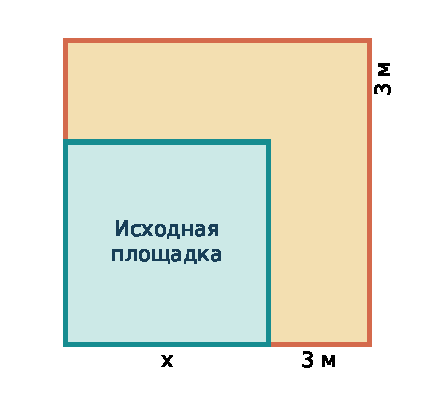
\includegraphics[width=.7\linewidth,height=45mm,keepaspectratio]{images/diagram-square.pdf}\end{center}
\Needspace{3\baselineskip}\item[\textbf{9.16.}\starmark] Упрости \(\frac{x^{2} - 9}{x^{2} - x - 6}\) и укажи ОДЗ исходного выражения.
\Needspace{3\baselineskip}\item[\textbf{9.17.}\starmark] Упрости: \((\frac{1}{x - 1} - \frac{1}{x + 1}) : (\frac{2}{x^{2} - 1})\).
\Needspace{3\baselineskip}\item[\textbf{9.18.}\starmark] Докажи тождество \((a + b)^{2} - (a - b)^{2} = 4 ab\) и проверь его при \(a = 103,\allowbreak b = 97\), не вычисляя квадраты больших чисел.
\Needspace{3\baselineskip}\item[\textbf{9.19.}] Докажите тождество \((a+b)^2+(a-b)^2=2a^2+2b^2\) для любых действительных \(a,b\).
\Needspace{3\baselineskip}\item[\textbf{9.20.}] Докажите, что при \(x\neq-1\) и \(x\neq1\) выполнено \(\frac1{x-1}-\frac1{x+1}=\frac2{x^2-1}\). Объясните, зачем нужны оба исключения.
\end{enumerate}

\chapter{Комбинаторика и бином Ньютона}\markright{Глава 10}
\section*{Сначала определите, какие результаты считаются разными}

\begin{definition}
\term{Комбинаторика} (combinatorics) изучает способы выбора и расположения элементов,
а также число таких способов. При подсчёте нужно явно установить,
различаются ли элементы, важен ли порядок и разрешены ли повторения.
\end{definition}

Например, выбор капитана и его заместителя из Анны и Бориса имеет два результата:
капитан Анна и заместитель Борис либо наоборот.
Выбор команды из этих же двух человек имеет один результат.
В первом случае порядок ролей важен, во втором --- нет.
Если из букв \(A,B,C\) составляют двухбуквенную последовательность с повторениями,
то \(AA\) допустима; без повторений --- нет.

\section*{Правила суммы и произведения}

\begin{theorem}[Правило суммы (sum rule)]
Если первая группа содержит \(m\) различных результатов, вторая --- \(n\),
и эти группы не пересекаются, то выбрать один результат
из их объединения можно \(m+n\) способами.
\end{theorem}
\begin{proof}Перечислим сначала \(m\) результатов первой группы, затем \(n\) результатов второй. Группы не пересекаются, поэтому все перечисленные результаты различны и их ровно \(m+n\).\end{proof}

Например, если на полке \(5\) разных романов и \(3\) разных учебника,
одну книгу можно выбрать \(5+3=8\) способами.
Условие непересечения существенно: один результат нельзя посчитать дважды.

\begin{theorem}[Правило произведения (product rule)]
Пусть выбор выполняется в несколько последовательных шагов.
Если на первом шаге есть \(n_1\) возможностей, после любого первого выбора
на втором есть ровно \(n_2\) возможностей, и так далее,
то полных последовательностей выборов ровно \(n_1n_2\cdots n_r\).
\end{theorem}
\par\addvspace{5pt}\begin{lrbox}{\CatFlowBox}\begin{minipage}[t]{\linewidth}
\setlength{\parskip}{5pt}\setlength{\columnsep}{4.5mm}\setlength{\intextsep}{0pt}
\begin{wrapfigure}[12]{l}{54mm}
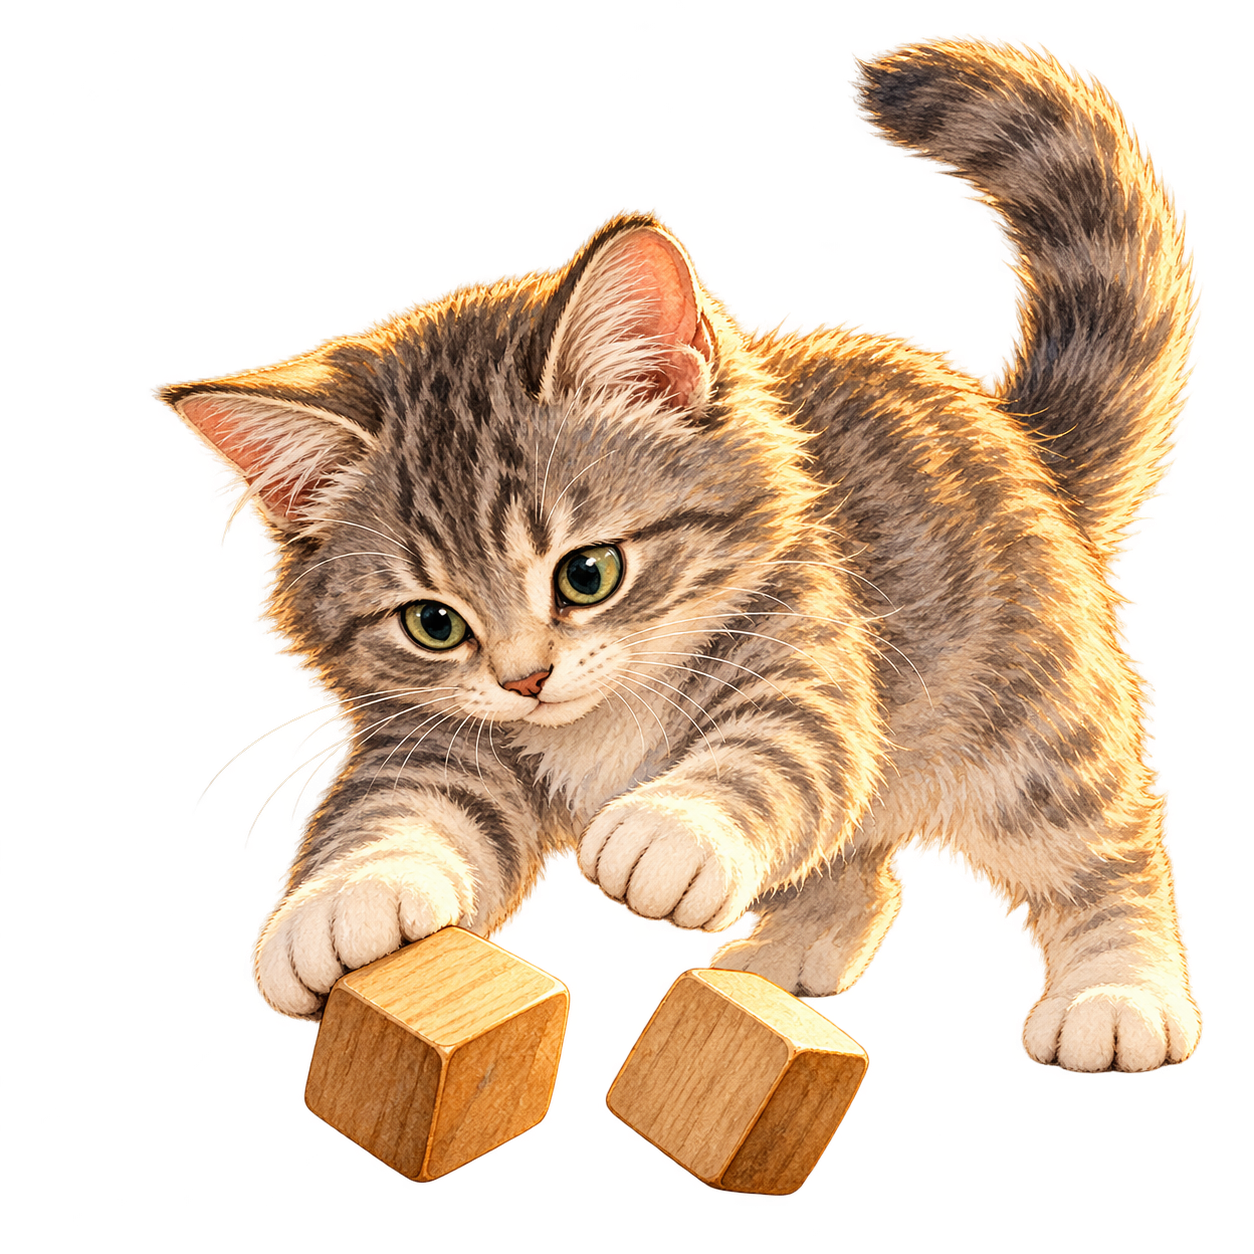
\includegraphics[width=54mm,height=58mm,keepaspectratio]{images/unique/art-17.png}
\end{wrapfigure}
\textit{Доказательство.} Для каждого результата первого шага имеется \(n_2\) продолжений. Получаются \(n_1\) непересекающихся групп по \(n_2\) исходов, всего \(n_1n_2\). Для большего числа шагов повторяем рассуждение, то есть применяем индукцию по числу шагов.\hfill\(\blacksquare\)

Например, к каждой из \(3\) рубашек можно надеть любые из \(2\) брюк:
получается \(3\cdot2=6\) комплектов.
Если число продолжений зависит от сделанного выбора, ветви сначала считают отдельно,
а затем складывают.
\par\WFclear\end{minipage}\end{lrbox}%
\ifdim\dimexpr\ht\CatFlowBox+\dp\CatFlowBox\relax<64mm\dp\CatFlowBox=\dimexpr64mm-\ht\CatFlowBox\relax\fi%
\noindent\usebox{\CatFlowBox}\par\addvspace{5pt}
\section*{Факториал и перестановки}

\begin{definition}
\term{Факториал} (factorial) натурального числа \(n\) --- произведение всех натуральных чисел от \(1\) до \(n\):
\[
n!=1\cdot2\cdots n.
\]
Дополнительно полагают \(0!=1\). Поэтому для \(n\in\mathbb N_0\)
\[
(n+1)!=(n+1)n!.
\]
\end{definition}

Значение \(0!=1\) соответствует одному способу расположить ноль элементов:
получить пустую последовательность. Например, \(4!=24\).

\begin{definition}
\term{Перестановка без повторений} (permutation without repetition) ---
расположение всех \(n\) различных элементов в определённом порядке.
\end{definition}

На первое место есть \(n\) вариантов, на второе --- \(n-1\), и так далее.
По правилу произведения число перестановок равно
\[
P_n=n!.
\]

\begin{definition}
\term{Перестановка с повторениями} (multiset permutation) ---
расположение \(n\) элементов, среди которых есть одинаковые:
\(n_1\) элементов первого вида, \(n_2\) второго и так далее,
где \(n_1+\cdots+n_r=n\).
\end{definition}

Число таких перестановок равно
\[
P(n_1,\ldots,n_r)=\frac{n!}{n_1!\cdots n_r!}.
\]
Действительно, если временно различить все одинаковые элементы,
каждое конечное расположение будет учтено \(n_1!\cdots n_r!\) раз.
Например, из букв слова «МАМА» получается \(\frac{4!}{2!2!}=6\) разных последовательностей.

\section*{Размещения: порядок важен}

\begin{definition}
\term{Размещение без повторений} (ordered selection without repetition) ---
упорядоченный выбор \(k\) различных элементов из \(n\) различных элементов.
\end{definition}

Для \(0\le k\le n\) число размещений равно
\[
A_n^k=\frac{n!}{(n-k)!}.
\]
При \(k\ge1\) это произведение \(k\) множителей:
\(n(n-1)\cdots(n-k+1)\); при \(k=0\) имеется один пустой выбор.
Например, капитана и заместителя из \(5\) человек выбирают \(A_5^2=5\cdot4=20\) способами.

\begin{definition}
\term{Размещение с повторениями} (ordered selection with repetition) ---
последовательность длины \(k\), каждый элемент которой выбирают из \(n\) видов;
один и тот же вид можно выбирать несколько раз.
\end{definition}

При \(n\ge1\), \(k\in\mathbb N_0\) число таких последовательностей равно
\[
\overline A_n^k=n^k.
\]
Например, двухсимвольных кодов из букв \(A,B,C\) ровно \(3^2=9\):
\(AA,AB,AC,BA,BB,BC,CA,CB,CC\).

\section*{Сочетания: порядок не важен}

\begin{definition}
\term{Сочетание без повторений} (combination without repetition) ---
выбор \(k\) элементов из \(n\) различных элементов, при котором порядок не учитывается
и каждый элемент выбирают не более одного раза.
\end{definition}

Каждый такой выбор порождает \(k!\) размещений, поэтому
\[
C_n^k=\binom nk=\frac{n!}{k!(n-k)!},\qquad 0\le k\le n.
\]
Например, пару участников из \(5\) человек выбирают \(\binom52=10\) способами.
Здесь обмен участников местами не создаёт новую пару.

\begin{definition}
\term{Сочетание с повторениями} (combination with repetition) ---
выбор \(k\) элементов из \(n\) видов, при котором порядок не учитывается,
а элементы каждого вида можно брать в любом количестве.
\end{definition}

При \(n\ge1\), \(k\in\mathbb N_0\) число таких выборов равно
\[
\overline C_n^k=\binom{n+k-1}{k}=\binom{n+k-1}{n-1}.
\]
Выбор задаётся количествами \(x_1,\ldots,x_n\) элементов каждого вида:
\(x_i\in\mathbb N_0\), \(x_1+\cdots+x_n=k\).
Чтобы увидеть формулу, расположим в строку \(k\) одинаковых звёздочек и \(n-1\) перегородок.
Количество звёздочек до первой перегородки задаёт \(x_1\), между первой и второй --- \(x_2\), и так далее.
Перегородки могут стоять рядом и по краям: это соответствует нулевым количествам.
Нужно выбрать позиции \(n-1\) перегородок среди \(n+k-1\) позиций.
Например, для \(3\) видов и \(4\) элементов получается \(\binom62=15\) выборов.

\section*{Биномиальные коэффициенты}

\begin{definition}
\term{Биномиальный коэффициент} (binomial coefficient) \(\binom nk\)
--- число сочетаний без повторений из \(n\) элементов по \(k\).
\end{definition}

Непосредственно из смысла выбора следуют равенства
\[
\binom n0=\binom nn=1,\qquad
\binom nk=\binom n{n-k}.
\]
Последнее равенство выражает соответствие между выбранными \(k\) элементами
и \(n-k\) оставшимися.

\begin{theorem}[Тождество Паскаля (Pascal's identity)]
Для целых \(n\ge1\), \(1\le k\le n\)
\[
\binom{n+1}k=\binom n{k-1}+\binom nk.
\]
\end{theorem}

\begin{proof}
Выделим один элемент из \(n+1\) различных элементов.
Если он входит в выбранную группу из \(k\) элементов,
остальных участников выбирают \(\binom n{k-1}\) способами.
Если не входит, всю группу выбирают \(\binom nk\) способами.
Эти случаи не пересекаются и охватывают все группы; применяем правило суммы.
\end{proof}

\section*{Бином Ньютона}

\begin{theorem}[Бином Ньютона (binomial theorem)]
Для любых рациональных чисел \(a,b\) и любого натурального \(n\)
\[
(a+b)^n=a^n+\sum_{k=1}^{n-1}\binom nk a^{n-k}b^k+b^n.
\]
Знак \(\sum\) означает сложение слагаемых при всех указанных значениях индекса \(k\).
При \(n=1\) внутренняя сумма пуста и равна нулю, так что формула даёт \(a+b=a+b\).
\end{theorem}

\par\addvspace{5pt}\begin{lrbox}{\CatFlowBox}\begin{minipage}[t]{\linewidth}
\setlength{\parskip}{5pt}\setlength{\columnsep}{4.5mm}\setlength{\intextsep}{0pt}
\begin{wrapfigure}[12]{r}{54mm}

\includegraphics[width=54mm,height=58mm,keepaspectratio]{images/unique/art-18.png}
\end{wrapfigure}
\textit{Доказательство.} Раскроем произведение \(n\) одинаковых скобок \((a+b)\).
В каждом слагаемом из каждой скобки выбран либо \(a\), либо \(b\).
Если при \(1\le k\le n-1\) число \(b\) выбрано ровно из \(k\) скобок,
а \(a\) --- из остальных, получается \(a^{n-k}b^k\).
Нужные \(k\) скобок можно выбрать \(\binom nk\) способами.
Выбор только \(a\) даёт \(a^n\), выбор только \(b\) --- \(b^n\).
Собирая одинаковые слагаемые, получаем формулу.\hfill\(\blacksquare\)
\par\WFclear\end{minipage}\end{lrbox}%
\ifdim\dimexpr\ht\CatFlowBox+\dp\CatFlowBox\relax<64mm\dp\CatFlowBox=\dimexpr64mm-\ht\CatFlowBox\relax\fi%
\noindent\usebox{\CatFlowBox}\par\addvspace{5pt}


Например,
\[
(a+b)^3=a^3+3a^2b+3ab^2+b^3.
\]
Запись с отдельно выписанными крайними слагаемыми позволяет применять формулу
и при \(a=0\) или \(b=0\), не вводя выражение \(0^0\).

\Needspace{7\baselineskip}\section*{Задачи}
\begingroup\setlength{\parskip}{3pt}
\noindent\begin{minipage}[t]{\linewidth}\textbf{10.1.} На полке стоят \(5\) разных романов и \(3\) разных учебника. Сколько есть способов выбрать одну книгу?\par\end{minipage}\par
\noindent\begin{minipage}[t]{\linewidth}\textbf{10.2.} Есть \(4\) рубашки, \(3\) пары брюк и \(2\) пары обуви. Любые вещи можно сочетать. Сколько комплектов из одной рубашки, одной пары брюк и одной пары обуви можно составить?\par\end{minipage}\par
\noindent\begin{minipage}[t]{\linewidth}\textbf{10.3.} Для каждого выбора укажи, важен ли порядок и разрешены ли повторения: а) распределить три призовых места между \(10\) участниками без ничьих; б) выбрать команду из \(3\) человек среди \(10\); в) составить код длины \(3\) из цифр \(0,\ldots,9\), допуская одинаковые цифры; г) выбрать \(3\) элемента из \(4\) видов, допуская один вид несколько раз и не учитывая порядок.\par\end{minipage}\par
\noindent\begin{minipage}[t]{\linewidth}\textbf{10.4.} Вычисли \(5!\), \(0!\) и \(\dfrac{7!}{5!}\).\par\end{minipage}\par
\noindent\begin{minipage}[t]{\linewidth}\textbf{10.5.} Сколькими способами можно расположить в ряд \(6\) различных книг, используя каждую ровно один раз?\par\end{minipage}\par
\noindent\begin{minipage}[t]{\linewidth}\textbf{10.6.} Сколько разных последовательностей можно получить, переставляя все буквы слова «ТОПОТ»? Осмысленность полученных слов не требуется.\par\end{minipage}\par
\noindent\begin{minipage}[t]{\linewidth}\textbf{10.7.} В забеге участвуют \(8\) человек. Сколько существует вариантов распределения первого, второго и третьего мест, если ничьи невозможны?\par\end{minipage}\par
\noindent\begin{minipage}[t]{\linewidth}\textbf{10.8.} Из \(8\) различных элементов выбирают \(3\), не учитывая порядок. Сколько существует выборов?\par\end{minipage}\par
\noindent\begin{minipage}[t]{\linewidth}\textbf{10.9.} Электронный замок принимает код из \(4\) цифр от \(0\) до \(9\). Повторения разрешены, первая цифра может быть нулём. Сколько разных кодов возможно?\par\end{minipage}\par
\noindent\begin{minipage}[t]{\linewidth}\textbf{10.10.} Сколько существует четырёхзначных натуральных чисел с попарно различными цифрами?\par\end{minipage}\par
\noindent\begin{minipage}[t]{\linewidth}\textbf{10.11.} Из \(4\) видов элементов выбирают \(3\) элемента. Каждый вид можно использовать сколько угодно раз, порядок не учитывается. Сколько существует выборов?\par\end{minipage}\par
\noindent\begin{minipage}[t]{\linewidth}\textbf{10.12.} Сколькими способами можно разложить \(7\) одинаковых шаров по \(3\) различным ящикам? Пустые ящики допускаются.\par\end{minipage}\par
\noindent\begin{minipage}[t]{\linewidth}\textbf{10.13.} Из множества, состоящего из \(n\ge2\) элементов, можно выбрать ровно \(45\) различных неупорядоченных пар. Найди \(n\).\par\end{minipage}\par
\par\addvspace{5pt}\begin{lrbox}{\CatFlowBox}\begin{minipage}[t]{\linewidth}
\setlength{\parskip}{5pt}\setlength{\columnsep}{4.5mm}\setlength{\intextsep}{0pt}
\begin{wrapfigure}[12]{l}{54mm}

\includegraphics[width=54mm,height=58mm,keepaspectratio]{images/unique/art-29.png}
\end{wrapfigure}
\textbf{10.14.} Пользуясь тождеством Паскаля и значениями \(\binom72=21\), \(\binom73=35\), вычисли \(\binom83\).\par

\textbf{10.15.} Раскрой скобки в \((x+2)^4\) с помощью бинома Ньютона.\par

\textbf{10.16.} Найди коэффициент при \(x^3\) после раскрытия скобок в \((2+x)^7\).\par

\textbf{10.17.} Докажи, что для любого \(n\in\mathbb N_0\) выполняется \(\sum_{k=0}^{n}\binom nk=2^n\).\par

\textbf{10.18.}\starmark{} Из \(4\) девушек и \(6\) юношей выбирают группу из \(5\) человек. Сколько существует групп, в которых не меньше двух девушек?\par

\textbf{10.19.}\starmark{} Сколько кодов длины \(5\) из цифр \(0,\ldots,9\) содержат хотя бы один ноль и хотя бы одну единицу? Начальный ноль разрешён, повторения разрешены.\par

\textbf{10.20.}\starmark{} Докажи подсчётом одного и того же множества двумя способами тождество Вандермонда: \(\sum_{k=0}^{r}\binom mk\binom n{r-k}=\binom{m+n}{r}\), где \(m,n\in\mathbb N_0\), \(0\le r\le m+n\). В этой задаче \(\binom uv=0\), если целое \(v<0\) или \(v>u\). Рассматривай целое \(r\in\mathbb N_0\).\par
\par\WFclear\end{minipage}\end{lrbox}%
\ifdim\dimexpr\ht\CatFlowBox+\dp\CatFlowBox\relax<64mm\dp\CatFlowBox=\dimexpr64mm-\ht\CatFlowBox\relax\fi%
\noindent\usebox{\CatFlowBox}\par\addvspace{5pt}

\endgroup

\chapter{Уравнения, системы и неравенства}
\begin{definition}\term{Корень уравнения} (\emph{root; solution of an equation}) — допустимое значение неизвестного, при котором равенство верно.\end{definition}
\begin{definition}\term{Решение неравенства} (\emph{solution of an inequality}) — значение неизвестного, при котором указанное сравнение верно.\end{definition}
\begin{definition}\term{Решение системы} (\emph{solution of a system}) — значения неизвестных, которые удовлетворяют всем её условиям одновременно.\end{definition}
\section*{Линейные и квадратные уравнения}
\(ax + b = 0\) при \(a \ne  0\) имеет корень \(x = - \frac{b}{a}\). При \(a = 0,\allowbreak b = 0\) подходят все \(x\); при \(a = 0,\allowbreak b \ne  0\) решений нет.\par
\begin{definition}\term{Дискриминант} (\emph{discriminant}) квадратного уравнения \(ax^{2}+bx+c=0\) при \(a\ne0\) — число \(D=b^{2}-4ac\).\end{definition}
При \(D > 0\) два корня: \(x = \frac{- b \pm  \sqrt{D}}{2 a}\). При \(D = 0\) один корень: \(- \frac{b}{2 a}\). При \(D < 0\) действительных корней нет.\par
\section*{Правила и проверка}
К обеим частям равенства или неравенства можно прибавить одно и то же выражение при сохранении ОДЗ.\par
При умножении или делении неравенства на отрицательное число знак меняется; на положительное — сохраняется.\par
Метод интервалов: отметь нули и запрещённые точки, определи знак на каждом участке и отдельно проверь включение границ.\par
При возведении уравнения в квадрат могут появиться посторонние корни: проверь найденные значения в исходном условии.\par
{\small\textit{Пример: \(- 2 x > 6\) даёт \(x < - 3\). Уравнение \(\sqrt{x + 2} = x\) требует \(x \ge  0\) ещё до возведения в квадрат.}}\par

% Дополнение к главе 15. Только действительные решения; формулы Кардано и Феррари не используются.
\subsection*{Многочлены и уравнения третьей степени}
\begin{definition}
\term{Многочлен} (polynomial) от \(x\) — выражение
\[
P(x)=a_nx^n+a_{n-1}x^{n-1}+\cdots+a_1x+a_0.
\]
Если \(a_n\neq0\), число \(n\) называют \term{степенью многочлена} (degree). \term{Корень многочлена} (polynomial root) — число \(r\), для которого \(P(r)=0\).
\end{definition}

\begin{definition}
Корень \(r\) имеет \term{кратность} (multiplicity) \(k\), если \(P(x)=(x-r)^kQ(x)\), где \(Q(r)\neq0\). При \(k=1\) корень называют простым, при \(k>1\) — кратным.
\end{definition}

\begin{theorem}[Сумма и разность кубов]
Для любых действительных \(a,b\)
\[
a^3-b^3=(a-b)(a^2+ab+b^2),\qquad
a^3+b^3=(a+b)(a^2-ab+b^2).
\]
\end{theorem}
\begin{proof}
При раскрытии скобок в первом произведении получаем
\(a^3+a^2b+ab^2-a^2b-ab^2-b^3=a^3-b^3\).
Во втором произведении средние слагаемые также сокращаются:
\(a^3-a^2b+ab^2+a^2b-ab^2+b^3=a^3+b^3\).
\end{proof}

\begin{theorem}[Теорема Безу]
\term{Теорема Безу} (factor theorem): для любого действительного \(r\) существует многочлен \(Q(x)\), для которого
\[
P(x)=(x-r)Q(x)+P(r).
\]
Следовательно, \(r\) — корень \(P\) тогда и только тогда, когда \(P(x)\) делится на \(x-r\) без остатка.
\end{theorem}
\begin{proof}
Для натурального \(k\)
\[
x^k-r^k=(x-r)(x^{k-1}+x^{k-2}r+\cdots+r^{k-1}).
\]
Равенство проверяется умножением: все промежуточные слагаемые сокращаются. Поэтому каждое слагаемое суммы \(P(x)-P(r)=\sum_{k=1}^n a_k(x^k-r^k)\) делится на \(x-r\). Это даёт нужный \(Q\). Если \(P(r)=0\), остаток равен нулю. Обратно, подставив \(x=r\) в \(P(x)=(x-r)Q(x)\), получаем \(P(r)=0\).
\end{proof}

\begin{theorem}[Рациональный корень]
Пусть коэффициенты \(P(x)=a_nx^n+\cdots+a_0\) целые, \(a_n\neq0\), \(a_0\neq0\). Если \(\frac pq\) — \term{рациональный корень} (rational root), причём \(p,q\) взаимно просты и \(q>0\), то \(p\) делит \(a_0\), а \(q\) делит \(a_n\).
\end{theorem}
\begin{proof}
Подстановка \(\frac pq\) и умножение на \(q^n\) дают
\[
a_np^n+a_{n-1}p^{n-1}q+\cdots+a_1pq^{n-1}+a_0q^n=0.
\]
Все слагаемые, кроме последнего, делятся на \(p\), поэтому \(p\) делит \(a_0q^n\). Поскольку \(p\) и \(q^n\) взаимно просты, \(p\) делит \(a_0\). Аналогично \(q\) делит \(a_np^n\), а значит, делит \(a_n\). Использованное свойство взаимной простоты следует из разложения на простые множители: множители делителя, отсутствующие в одном сомножителе, должны целиком входить в другой.
\end{proof}

Если старший коэффициент равен \(1\), рациональный корень может быть только целым делителем свободного члена. Проверяем кандидатов подстановкой, а найденный множитель \(x-r\) отделяем по теореме Безу. Если свободный член нулевой, сначала выносим \(x\). Отсутствие рациональных корней не означает отсутствия действительных: например, \(x^3-2=0\) имеет корень \(\sqrt[3]2\).

\begin{example}
Для \(P(x)=x^3-4x^2+x+6\) проверка даёт \(P(2)=0\). Поэтому
\[
P(x)=(x-2)(x^2-2x-3)=(x-2)(x-3)(x+1).
\]
Уравнение \(P(x)=0\) имеет корни \(-1,2,3\).
\end{example}

\begin{theorem}[Устранение квадратного слагаемого]
В \term{кубическом уравнении} (cubic equation)
\(ax^3+bx^2+cx+d=0\), где \(a\neq0\), замена \(x=t-\frac{b}{3a}\) даёт \term{неполное кубическое уравнение} (depressed cubic)
\[
t^3+pt+q=0,\qquad
p=\frac{3ac-b^2}{3a^2},\qquad
q=\frac{2b^3-9abc+27a^2d}{27a^3}.
\]
\end{theorem}
\begin{proof}
После деления на \(a\) обозначим коэффициенты через \(B=\frac ba\), \(C=\frac ca\), \(D=\frac da\). Подставим \(x=t-\frac B3\) и раскроем скобки:
\[
\begin{aligned}
&\left(t-\frac B3\right)^3+B\left(t-\frac B3\right)^2+C\left(t-\frac B3\right)+D\\
&\qquad=t^3+\left(C-\frac{B^2}{3}\right)t+\frac{2B^3}{27}-\frac{BC}{3}+D.
\end{aligned}
\]
Коэффициент при \(t^2\) равен нулю. Подстановка \(B,C,D\) даёт указанные \(p,q\).
\end{proof}

Такая замена упрощает форму уравнения; сама по себе она не даёт готовой формулы корней. В задачах этого раздела после замены достаточно разложения на множители или выделения куба.

\subsection*{Два вида уравнений четвёртой степени}
\begin{definition}
\term{Биквадратное уравнение} (biquadratic equation) имеет вид \(ax^4+bx^2+c=0\), где \(a\neq0\). Замена \(u=x^2\) приводит к квадратному уравнению \(au^2+bu+c=0\) с обязательным условием \(u\geq0\).
\end{definition}
Каждое \(u>0\) даёт два корня \(x=\pm\sqrt u\), значение \(u=0\) — один корень \(x=0\), а отрицательное \(u\) действительных корней не даёт.

\begin{example}
\(x^4-10x^2+9=0\) после замены \(u=x^2\) даёт \((u-1)(u-9)=0\). Поэтому \(x=-3,-1,1,3\).
\end{example}

\begin{definition}
\term{Возвратное уравнение четвёртой степени} (reciprocal quartic equation) в этом разделе — уравнение
\[
ax^4+bx^3+cx^2+bx+a=0,\qquad a\neq0,
\]
у которого коэффициенты симметричны относительно середины.
\end{definition}

\begin{theorem}[Замена для возвратного уравнения]
Корни указанного возвратного уравнения ненулевые. Замена \(t=x+\frac1x\) сводит поиск действительных корней к
\[
at^2+bt+c-2a=0,\qquad |t|\geq2.
\]
Для каждого допустимого \(t\) решают \(x^2-tx+1=0\).
\end{theorem}
\begin{proof}
При \(x=0\) левая часть исходного уравнения равна \(a\neq0\), поэтому деление на \(x^2\) допустимо. Получаем
\[
a\left(x^2+\frac1{x^2}\right)+b\left(x+\frac1x\right)+c=0.
\]
Из \(t=x+\frac1x\) следует \(x^2+\frac1{x^2}=t^2-2\), что даёт квадратное уравнение для \(t\). Обратная подстановка равносильна \(x^2-tx+1=0\). Его дискриминант \(t^2-4\) неотрицателен ровно при \(|t|\geq2\); свободный член \(1\) исключает нулевой корень. Значит, указанное условие необходимо и достаточно.
\end{proof}

\begin{example}
Для \(x^4-3x^3+2x^2-3x+1=0\) получаем \(t^2-3t=0\), то есть \(t=0\) или \(t=3\). Значение \(t=0\) не удовлетворяет \(|t|\geq2\). При \(t=3\) имеем \(x^2-3x+1=0\), откуда
\[
x=\frac{3-\sqrt5}{2}\quad\text{или}\quad x=\frac{3+\sqrt5}{2}.
\]
\end{example}

\Needspace{7\baselineskip}\section*{Задачи}
\begin{enumerate}[label={},leftmargin=3.2em,itemsep=10pt]
\Needspace{3\baselineskip}\item[\textbf{11.1.}] Реши \(3 x - 7 = 11\).
\Needspace{3\baselineskip}\item[\textbf{11.2.}] Реши \(2 (x - 3) = 5 x + 9\).
\Needspace{3\baselineskip}\item[\textbf{11.3.}] Реши \(x^{2} - 5 x + 6 = 0\).
\Needspace{3\baselineskip}\item[\textbf{11.4.}] Реши \(2 x^{2} - 8 = 0\).
\Needspace{3\baselineskip}\item[\textbf{11.5.}] Реши \(\frac{x + 1}{x - 2} = 2\).
\Needspace{3\baselineskip}\item[\textbf{11.6.}] Реши систему: \(x + y = 7;\allowbreak x - y = 1\).
\Needspace{3\baselineskip}\item[\textbf{11.7.}] Реши \(- 3 x > 12\).
\Needspace{3\baselineskip}\item[\textbf{11.8.}] Реши \(x^{2} - 9 \le  0\).
\Needspace{3\baselineskip}\item[\textbf{11.9.}] Реши \((x - 1) (x + 2) > 0\).
\Needspace{3\baselineskip}\item[\textbf{11.10.}] Реши \(\frac{x - 3}{x + 1} \le  0\).
\Needspace{3\baselineskip}\item[\textbf{11.11.}] Реши \(| 2 x - 1 | = 5\).
\Needspace{3\baselineskip}\item[\textbf{11.12.}] Реши \(\sqrt{x + 2} = x\).
\Needspace{3\baselineskip}\item[\textbf{11.13.}] Из жизни. Поездка на такси стоит \(150\) рублей за подачу и \(30\) рублей за километр. Счёт составил \(510\) рублей. Какое расстояние проехали?
\Needspace{3\baselineskip}\item[\textbf{11.14.}] Из жизни. За \(3\) одинаковых блокнота и ручку стоимостью \(80\) рублей заплатили \(440\) рублей. Сколько стоит блокнот?
\Needspace{3\baselineskip}\item[\textbf{11.15.}] Из жизни. Для покупки билетов по \(350\) рублей выделено \(2000\) рублей. Какое максимальное целое число билетов можно купить?
\Needspace{3\baselineskip}\item[\textbf{11.16.}\starmark] Реши \(\sqrt{2 x + 3} = x\).
\Needspace{3\baselineskip}\item[\textbf{11.17.}\starmark] Реши \(\frac{x - 2}{x + 3} \ge  1\).
\Needspace{3\baselineskip}\item[\textbf{11.18.}\starmark] У прямоугольного участка периметр \(34\) м, площадь \(60\) м\(^{2}\). Найди стороны.
\Needspace{3\baselineskip}\item[\textbf{11.19.}] Докажите формулы Виета: если \(x_1,x_2\) — действительные корни \(ax^2+bx+c=0\), \(a\neq0\), с учётом кратности, то \(x_1+x_2=-\frac ba\), \(x_1x_2=\frac ca\).
\Needspace{3\baselineskip}\item[\textbf{11.20.}] Докажите, что квадратное уравнение \(ax^2+bx+c=0\), \(a\neq0\), имеет действительный корень тогда и только тогда, когда \(D=b^2-4ac\geq0\). Используйте выделение полного квадрата.
\Needspace{3\baselineskip}\item[\textbf{11.21.}] Решите в действительных числах \(x^3-8=0\), разложив разность кубов на множители.
\Needspace{3\baselineskip}\item[\textbf{11.22.}] Решите в действительных числах \(x^3+27=0\), разложив сумму кубов на множители.
\Needspace{3\baselineskip}\item[\textbf{11.23.}] Решите \(x^3-6x^2+11x-6=0\). Найдите целый корень, затем выделите соответствующий линейный множитель.
\Needspace{3\baselineskip}\item[\textbf{11.24.}] Решите \(2x^3-3x^2-8x+12=0\) в действительных числах.
\Needspace{3\baselineskip}\item[\textbf{11.25.}\starmark] В уравнении \(x^3-6x^2+9x-4=0\) сделайте замену \(x=t+2\). Решите полученное уравнение и вернитесь к \(x\).
\Needspace{3\baselineskip}\item[\textbf{11.26.}] Решите биквадратное уравнение \(x^4-5x^2+4=0\).
\Needspace{3\baselineskip}\item[\textbf{11.27.}] Решите в действительных числах \(x^4+3x^2-4=0\), проверив допустимость найденных значений \(x^2\).
\Needspace{3\baselineskip}\item[\textbf{11.28.}\starmark] Решите возвратное уравнение \(x^4-5x^3+6x^2-5x+1=0\). Для каждого корня уравнения относительно \(t=x+\frac1x\) проверьте условие \(|t|\geq2\).
\end{enumerate}

\chapter{Последовательности и прогрессии}\markright{Глава 12}
\begin{definition}
\term{Числовая последовательность} (real sequence) — отображение \(a:\mathbb N\to\mathbb R\), где \(\mathbb N=\{1,2,3,\ldots\}\). Числу \(n\) соответствует \term{член последовательности} (term) \(a_n\); \(n\) — его номер. Последовательность записывают как \((a_n)_{n\geq1}\).
\end{definition}
\begin{definition}
\term{Формула общего члена} (explicit formula) непосредственно выражает \(a_n\) через \(n\). \term{Рекуррентная, или индуктивная, запись} (recursive definition) задаёт начальное значение и правило получения следующих членов из предыдущих. Например, \(a_1=2\), \(a_{n+1}=a_n+3\) при \(n\geq1\).
\end{definition}
\begin{definition}
\term{Арифметическая прогрессия} (arithmetic progression) — последовательность, для которой \(a_{n+1}=a_n+d\) при всех \(n\geq1\). Постоянное число \(d\) называют \term{разностью прогрессии} (common difference).
\end{definition}
\begin{theorem}[Общий член арифметической прогрессии]
Для арифметической прогрессии
\[
a_n=a_1+(n-1)d,\qquad n\geq1.
\]
\end{theorem}
\begin{proof}
При \(n=1\) равенство верно. Если \(a_k=a_1+(k-1)d\), то \(a_{k+1}=a_k+d=a_1+kd\). По математической индукции формула верна для всех \(n\geq1\).
\end{proof}
\begin{definition}
\term{Частичная сумма} (partial sum) последовательности — сумма первых \(N\) членов: \(S_N=a_1+\cdots+a_N\).
\end{definition}
\begin{theorem}[Сумма арифметической прогрессии]
\[
S_N=\frac{N(a_1+a_N)}{2}=\frac N2\bigl(2a_1+(N-1)d\bigr).
\]
\end{theorem}
\par\addvspace{5pt}\begin{lrbox}{\CatFlowBox}\begin{minipage}[t]{\linewidth}
\setlength{\parskip}{5pt}\setlength{\columnsep}{4.5mm}\setlength{\intextsep}{0pt}
\begin{wrapfigure}[12]{l}{54mm}
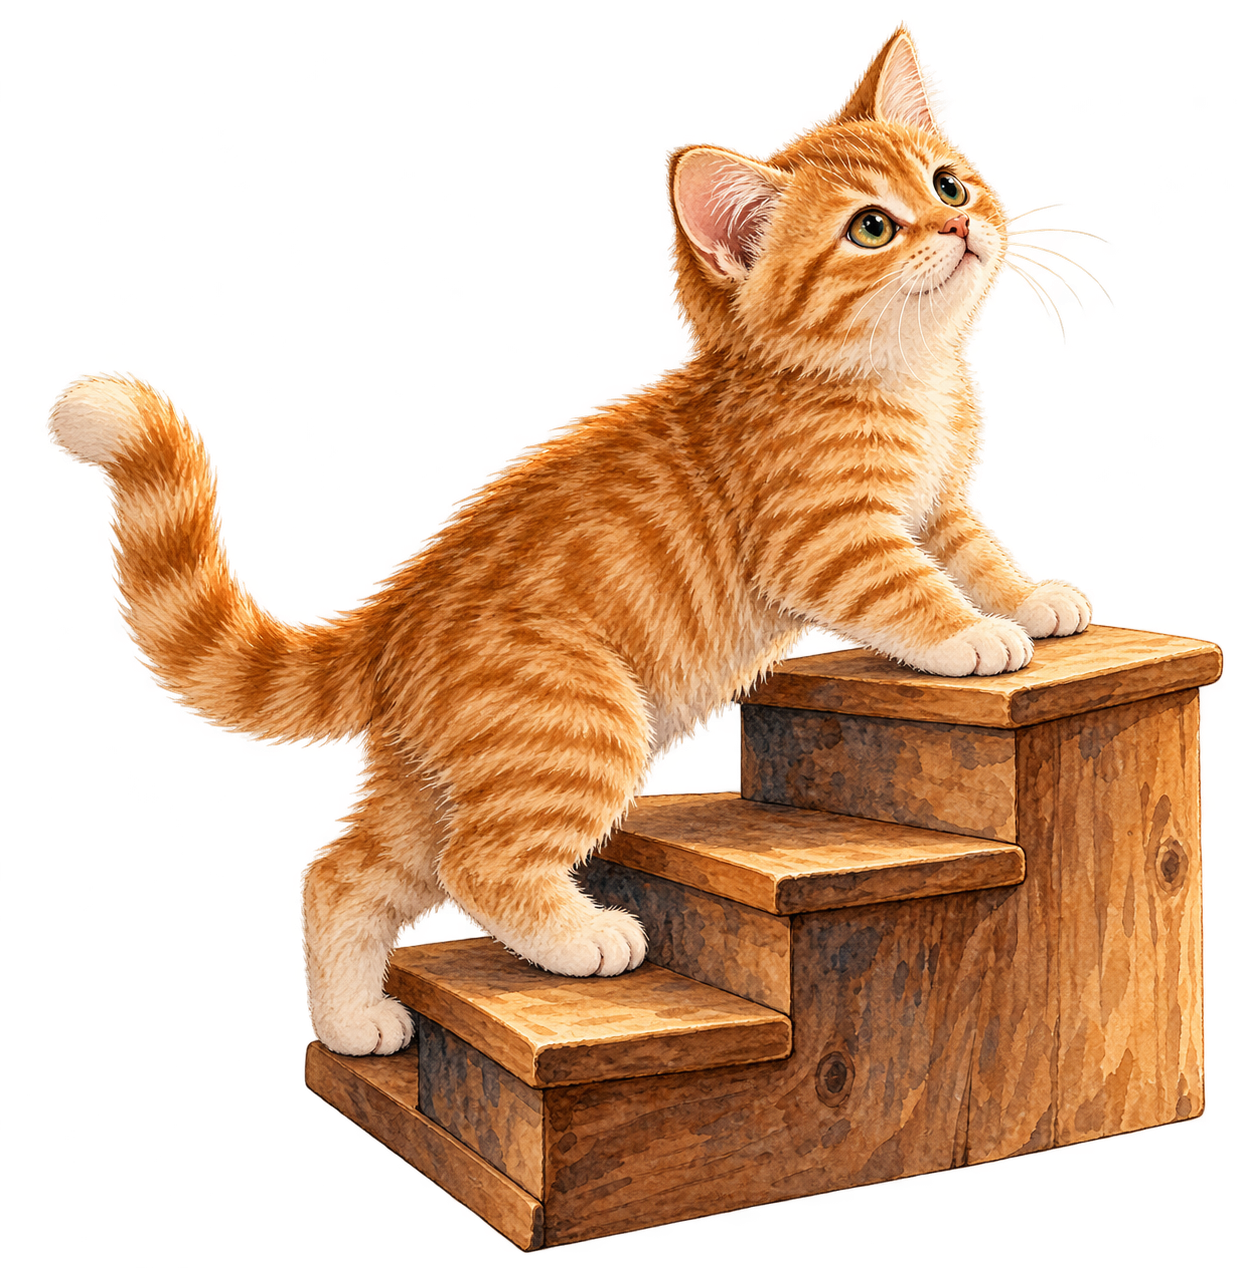
\includegraphics[width=54mm,height=58mm,keepaspectratio]{images/unique/art-13.png}
\end{wrapfigure}
\textit{Доказательство.} Запишем одну и ту же сумму в прямом и обратном порядке. При сложении получим \(2S_N=(a_1+a_N)+(a_2+a_{N-1})+\cdots+(a_N+a_1)\). В каждой из \(N\) скобок сумма равна \(2a_1+(N-1)d=a_1+a_N\). Деление на \(2\) даёт первую формулу, а подстановка общего члена — вторую. Рассуждение не зависит от чётности \(N\).\hfill\(\square\)
\par\WFclear\end{minipage}\end{lrbox}%
\ifdim\dimexpr\ht\CatFlowBox+\dp\CatFlowBox\relax<64mm\dp\CatFlowBox=\dimexpr64mm-\ht\CatFlowBox\relax\fi%
\noindent\usebox{\CatFlowBox}\par\addvspace{5pt}

\begin{definition}
\term{Геометрическая прогрессия} (geometric progression) в этом сборнике — последовательность, для которой \(a_{n+1}=q a_n\) при всех \(n\geq1\). Постоянное число \(q\) называют \term{знаменателем прогрессии} (common ratio). Такое определение включает \(q=0\): тогда последовательность имеет вид \(a_1,0,0,\ldots\).
\end{definition}
\begin{theorem}[Общий член геометрической прогрессии]
При \(q\neq0\)
\[
a_n=a_1q^{n-1},\qquad n\geq1.
\]
При \(q=0\) отдельно имеем \(a_n=0\) для \(n\geq2\); значение \(a_1\) задано начальным условием.
\end{theorem}
\begin{proof}
При \(q\neq0\) база \(n=1\) даёт \(a_1q^0=a_1\). Из формулы для \(k\) следует \(a_{k+1}=q a_k=q a_1q^{k-1}=a_1q^k\). При \(q=0\) сначала \(a_2=0\), затем каждый следующий член равен \(0\cdot0=0\). Такое отдельное рассмотрение позволяет не использовать неопределённую запись \(0^0\).
\end{proof}
\begin{theorem}[Сумма геометрической прогрессии]
При \(q\neq1\)
\[
S_N=\frac{a_1(1-q^N)}{1-q}.
\]
При \(q=1\) имеем \(S_N=Na_1\). Формула для \(q\neq1\) верна также при \(q=0\).
\end{theorem}
\begin{proof}
Из рекуррентного правила
\(qS_N=a_2+a_3+\cdots+a_{N+1}\). Вычитая это равенство из \(S_N=a_1+a_2+\cdots+a_N\), получаем \((1-q)S_N=a_1-a_{N+1}=a_1(1-q^N)\). При \(q\neq1\) делим на \(1-q\). При \(q=1\) все члены равны \(a_1\), поэтому сумма равна \(Na_1\).
\end{proof}
\subsection*{Предел, монотонность и ограниченность}
\begin{definition}
Число \(L\) — \term{предел последовательности} (limit of a sequence) \((b_N)\), если для любого \(\varepsilon>0\) существует натуральное \(N_0\), такое что при всех \(N\geq N_0\) выполнено \(|b_N-L|<\varepsilon\). Запись: \(\lim_{N\to\infty}b_N=L\). Иными словами, все достаточно поздние члены попадают в любой заранее выбранный интервал вокруг \(L\).
\end{definition}
\begin{definition}
Последовательность \((a_n)\) \term{не убывает} (is nondecreasing), если \(a_{n+1}\geq a_n\) для всех \(n\), и \term{не возрастает} (is nonincreasing), если \(a_{n+1}\leq a_n\). В обоих случаях её называют \term{монотонной} (monotone). Если неравенства строгие, говорят о строго возрастающей или строго убывающей последовательности.
\end{definition}
\begin{definition}
Последовательность \term{ограничена сверху} (bounded above), если существует число \(M\), такое что \(a_n\leq M\) при всех \(n\). Она \term{ограничена снизу} (bounded below), если существует \(m\) с \(m\leq a_n\) при всех \(n\). Если выполнены оба условия, последовательность \term{ограничена} (bounded).
\end{definition}
\begin{definition}
Число \(L\) называют \term{супремумом, или точной верхней гранью} (supremum, least upper bound) непустого множества \(A\subseteq\mathbb R\), если \(a\leq L\) для всех \(a\in A\), но никакое меньшее число не обладает этим свойством. Обозначение: \(L=\sup A\).
\end{definition}
\begin{definition}
Число \(m\) — \term{нижняя грань} (lower bound) множества \(A\subseteq\mathbb R\), если \(m\le a\) для каждого \(a\in A\).\end{definition}
\begin{definition}\term{Инфимум, или точная нижняя грань} (infimum; greatest lower bound) непустого множества — наибольшая его нижняя грань. Обозначение: \(\inf A\). Инфимум не обязан принадлежать самому множеству.
\end{definition}
Для \(A=(0;1]\) имеем \(\inf A=0\), \(\sup A=1\). Наименьшего элемента нет, а наибольший равен \(1\). Нельзя путать нижнюю грань с наименьшим элементом: граница описывает всё множество и может лежать вне него.
\begin{axiom}[Полнота действительных чисел]
\term{Аксиома полноты} (completeness axiom): каждое непустое множество действительных чисел, ограниченное сверху, имеет действительный супремум.
\end{axiom}
\begin{theorem}[Существование инфимума]
Всякое непустое ограниченное снизу множество \(A\subseteq\mathbb R\) имеет инфимум. Если \(-A=\{-a:a\in A\}\), то \(\inf A=-\sup(-A)\).
\end{theorem}
\begin{proof}
Множество \(-A\) непусто и ограничено сверху. Пусть \(L=\sup(-A)\), существующий по полноте. Из \(-a\le L\) получаем \(-L\le a\), так что \(-L\) — нижняя грань \(A\). Если \(b\) — любая нижняя грань, то \(-b\) — верхняя грань \(-A\), откуда \(L\le-b\), то есть \(b\le-L\). Следовательно, \(-L\) — наибольшая нижняя грань.
\end{proof}
\begin{theorem}[Сходимость монотонной ограниченной последовательности]
Всякая неубывающая и ограниченная сверху последовательность сходится. Её предел равен \(L=\sup\{a_n:n\in\mathbb N\}\). Всякая невозрастающая и ограниченная снизу последовательность также сходится. Следовательно, любая монотонная ограниченная последовательность имеет конечный предел.
\end{theorem}
\par\addvspace{5pt}\begin{lrbox}{\CatFlowBox}\begin{minipage}[t]{\linewidth}
\setlength{\parskip}{5pt}\setlength{\columnsep}{4.5mm}\setlength{\intextsep}{0pt}
\begin{wrapfigure}[12]{r}{54mm}
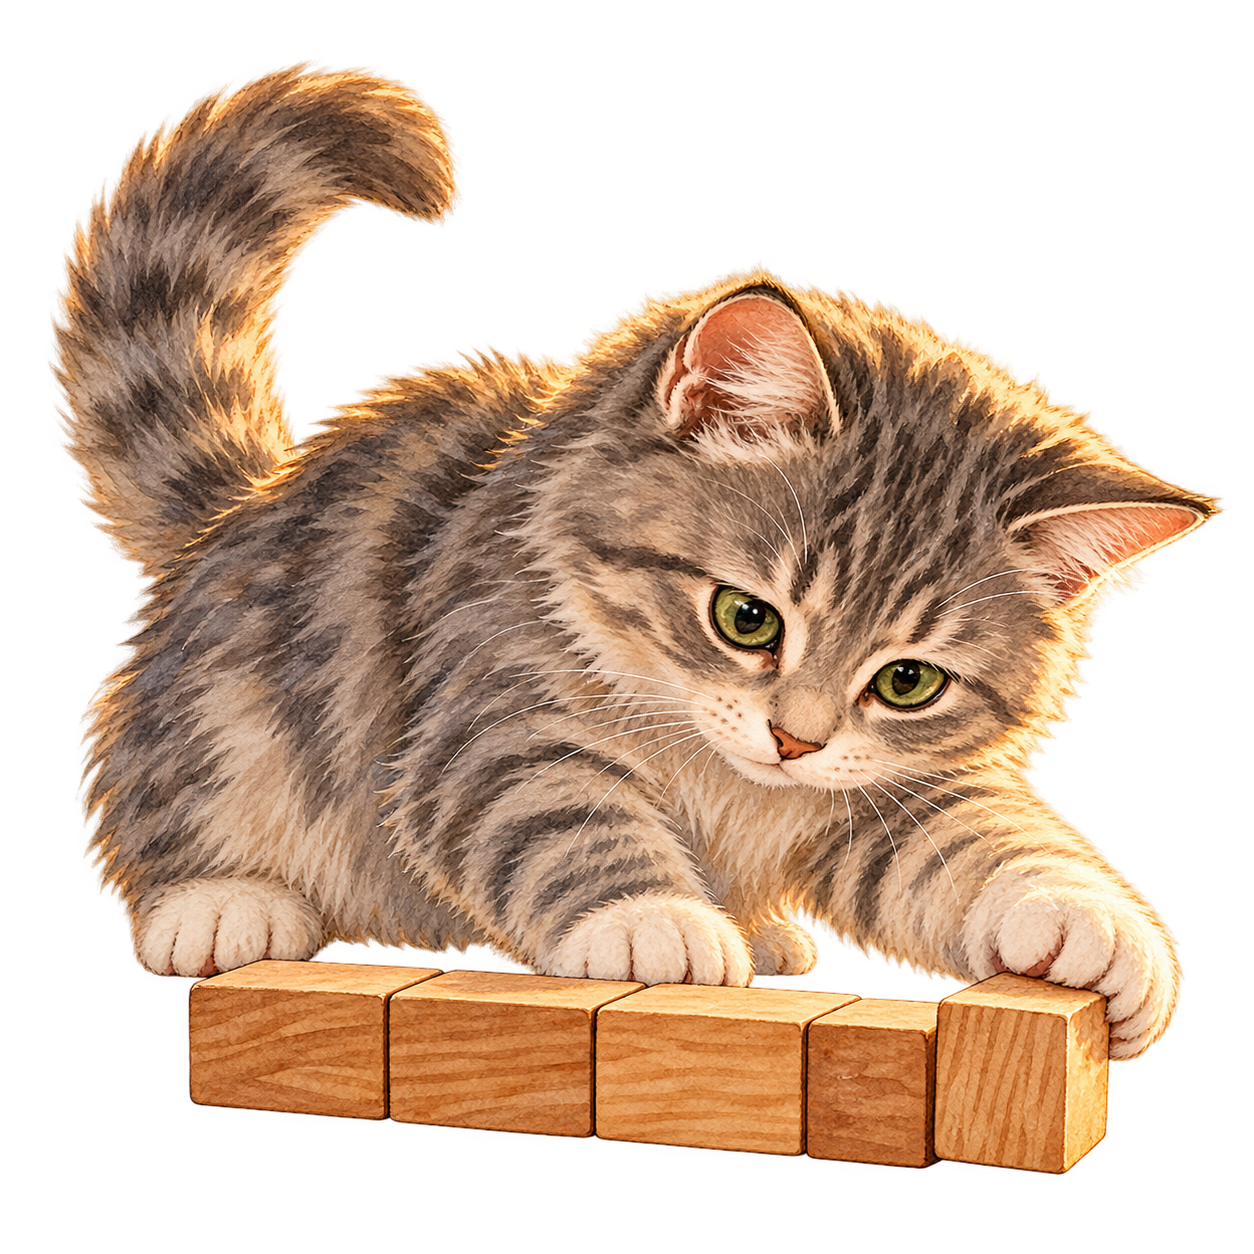
\includegraphics[width=54mm,height=58mm,keepaspectratio]{images/unique/art-20.png}
\end{wrapfigure}
\textit{Доказательство.} Для неубывающей последовательности супремум \(L\) существует по аксиоме полноты. Выберем любое \(\varepsilon>0\). Число \(L-\varepsilon\) не является верхней гранью, поэтому существует номер \(N\), для которого \(a_N>L-\varepsilon\). При всех \(n\geq N\) по монотонности \(a_n\geq a_N\), а по свойству верхней грани \(a_n\leq L\). Значит, \(L-\varepsilon<a_n\leq L\), то есть \(|a_n-L|<\varepsilon\). Это и означает \(a_n\to L\).

Для невозрастающей и ограниченной снизу последовательности \((a_n)\) последовательность \((-a_n)\) не убывает и ограничена сверху. Уже доказанный случай даёт \(-a_n\to B\), откуда \(a_n\to-B\), поскольку \(|a_n-(-B)|=|-a_n-B|\).\hfill\(\square\)
\par\WFclear\end{minipage}\end{lrbox}%
\ifdim\dimexpr\ht\CatFlowBox+\dp\CatFlowBox\relax<64mm\dp\CatFlowBox=\dimexpr64mm-\ht\CatFlowBox\relax\fi%
\noindent\usebox{\CatFlowBox}\par\addvspace{5pt}

Условие с \(\varepsilon\) придаёт словам «сколь угодно близко» точный смысл: сначала выбирается любая положительная точность \(\varepsilon\), и только после этого подбирается номер \(N\), начиная с которого \emph{все} члены удовлетворяют \(|a_n-L|<\varepsilon\). Единого заранее фиксированного \(N\) для всех точностей не требуется.

\subsection*{Бесконечная сумма}
\begin{definition}
\term{Бесконечный ряд} (infinite series) \(\sum_{n=1}^{\infty}a_n\) \term{сходится} (converges) к числу \(S\), если его частичные суммы \(S_N\) имеют предел \(S\). Число \(S\) называют \term{суммой ряда} (sum of a series). Если такого конечного предела нет, ряд \term{расходится} (diverges).
\end{definition}
\begin{theorem}[Бесконечная геометрическая сумма]
Пусть \(a_{n+1}=q a_n\). При \(|q|<1\)
\[
\sum_{n=1}^{\infty}a_n=\frac{a_1}{1-q}.
\]
Если \(a_1\neq0\), условие \(|q|<1\) также необходимо для сходимости. В частности, при \(q=1\) и при \(q=-1\) такой ряд расходится.
\end{theorem}
\begin{proof}
Сначала покажем \(q^N\to0\) при \(|q|<1\). Случай \(q=0\) непосредственен. Если \(0<r=|q|<1\), то \(r=\frac1{1+h}\) с \(h>0\). Неравенство \((1+h)^N\geq1+Nh\) доказывается индукцией: после умножения \(1+Nh\) на \(1+h\) получаем \(1+(N+1)h+Nh^2\geq1+(N+1)h\). Значит, \(|q^N|=r^N\leq\frac1{1+Nh}\), а эта верхняя граница становится меньше любого \(\varepsilon>0\) при достаточно большом \(N\).

По формуле конечной суммы
\[
\left|S_N-\frac{a_1}{1-q}\right|=\frac{|a_1|\,|q|^N}{|1-q|}\longrightarrow0.
\]
При \(a_1=0\) все суммы уже равны нулю. Если \(a_1\neq0\) и \(|q|\geq1\), то \(|a_n|=|a_1||q|^{n-1}\geq|a_1|\), поэтому \(a_n\) не стремится к нулю. Но из сходимости \(S_N\to S\) обязательно следует \(a_N=S_N-S_{N-1}\to0\): разность ограничена сверху величиной \(|S_N-S|+|S_{N-1}-S|\), и оба слагаемых стремятся к нулю. Получили противоречие.

Наглядно, при \(q=1\) суммы \(S_N=Na_1\) неограниченно растут по модулю. При \(q=-1\) они чередуются: \(S_{2k}=0\), \(S_{2k-1}=a_1\); при \(a_1\neq0\) единого предела нет.
\end{proof}
\begin{example}
\(1+\frac12+\frac14+\cdots=2\). При этом первые \(N\) слагаемых дают \(S_N=2(1-2^{-N})\), а недостающая до \(2\) величина равна \(2^{1-N}\) и стремится к нулю.
\end{example}

\Needspace{7\baselineskip}\section*{Задачи}
\begingroup\setlength{\parskip}{3pt}
\noindent\begin{minipage}[t]{\linewidth}\textbf{12.1.} Последовательность задана формулой \(a_n=3n-2\), \(n\geq1\). Выпишите первые пять членов и найдите \(a_{10}\).\par\end{minipage}\par
\noindent\begin{minipage}[t]{\linewidth}\textbf{12.2.} Для \(a_n=\dfrac{(-1)^n}{n}\) выпишите первые четыре члена. Укажите знак \(a_{25}\) и знак \(a_{26}\).\par\end{minipage}\par
\noindent\begin{minipage}[t]{\linewidth}\textbf{12.3.} Дано \(a_1=2\), \(a_{n+1}=2a_n-1\). Выпишите первые пять членов последовательности.\par\end{minipage}\par
\noindent\begin{minipage}[t]{\linewidth}\textbf{12.4.} Последовательность \(3,7,11,15,\ldots\) — арифметическая прогрессия. Найдите её разность и формулу общего члена.\par\end{minipage}\par
\noindent\begin{minipage}[t]{\linewidth}\textbf{12.5.} В арифметической прогрессии \(a_1=7\), \(d=-3\). Найдите \(a_8\).\par\end{minipage}\par
\noindent\begin{minipage}[t]{\linewidth}\textbf{12.6.} В арифметической прогрессии \(a_3=11\), \(a_9=35\). Найдите \(d\) и \(a_1\).\par\end{minipage}\par
\noindent\begin{minipage}[t]{\linewidth}\textbf{12.7.} Найдите сумму первых двадцати членов арифметической прогрессии с \(a_1=5\) и \(d=2\).\par\end{minipage}\par
\noindent\begin{minipage}[t]{\linewidth}\textbf{12.8.} Последовательность \(3,-6,12,-24,\ldots\) — геометрическая прогрессия. Найдите \(q\), формулу \(a_n\) и \(a_6\).\par\end{minipage}\par
\noindent\begin{minipage}[t]{\linewidth}\textbf{12.9.} В геометрической прогрессии \(a_1=81\), \(q=\dfrac13\). Найдите \(a_5\).\par\end{minipage}\par
\noindent\begin{minipage}[t]{\linewidth}\textbf{12.10.} В действительной геометрической прогрессии \(a_2=6\), \(a_5=48\). Найдите \(q\) и \(a_1\).\par\end{minipage}\par
\noindent\begin{minipage}[t]{\linewidth}\textbf{12.11.} Вычислите сумму \(1+2+4+\cdots+128\). Сначала определите число слагаемых.\par\end{minipage}\par
\noindent\begin{minipage}[t]{\linewidth}\textbf{12.12.} Найдите сумму бесконечного ряда \(18-6+2-\dfrac23+\cdots\). Объясните, почему геометрическая сумма здесь существует.\par\end{minipage}\par
\noindent\begin{minipage}[t]{\linewidth}\textbf{12.13.} В первую неделю в копилку положили \(100\) рублей, а в каждую следующую — на \(50\) рублей больше, чем в предыдущую. Сколько рублей положили за \(12\) недель?\par\end{minipage}\par
\noindent\begin{minipage}[t]{\linewidth}\textbf{12.14.} В первом ряду зала \(12\) мест, а в каждом следующем на \(2\) места больше. Всего \(20\) рядов. Найдите число мест в последнем ряду и во всём зале.\par\end{minipage}\par
\noindent\begin{minipage}[t]{\linewidth}\textbf{12.15.} В игре за первый день дают \(2\) монеты, а каждый следующий день награду удваивают. Найдите награду за седьмой день и общее число монет за первые семь дней.\par\end{minipage}\par
\par\addvspace{5pt}\begin{lrbox}{\CatFlowBox}\begin{minipage}[t]{\linewidth}
\setlength{\parskip}{5pt}\setlength{\columnsep}{4.5mm}\setlength{\intextsep}{0pt}
\begin{wrapfigure}[12]{l}{54mm}

\includegraphics[width=54mm,height=58mm,keepaspectratio]{images/unique/art-30.png}
\end{wrapfigure}
\textbf{12.16.} Докажите с помощью формулы суммы арифметической прогрессии, что \(1+3+5+\cdots+(2N-1)=N^2\) для любого натурального \(N\).\par

\textbf{12.17.} Докажите, что ряд \(a-a+a-a+\cdots\) не имеет суммы в смысле предела частичных сумм, если \(a\neq0\).\par

\textbf{12.18.}\starmark{} Дано \(a_1=3\), \(a_{n+1}=2a_n+1\). Найдите формулу общего члена и сумму первых десяти членов.\par

\textbf{12.19.}\starmark{} В арифметической прогрессии \(d>0\), \(a_2+a_5=34\), \(a_3a_4=280\). Найдите \(a_1\), \(d\) и \(S_{10}\).\par

\textbf{12.20.}\starmark{} Суммируют числа \(64,16,4,1,\ldots\). Найдите бесконечную сумму \(S\), формулу остатка \(R_N=S-S_N\) и наименьшее натуральное \(N\), при котором \(R_N<\dfrac1{10}\).\par

\textbf{12.21.} Для множества \((-2;5]\) найди супремум, инфимум, наибольший и наименьший элементы, если они существуют.\par

\textbf{12.22.} Найди точные грани множества \(A=\{1+\dfrac1n:n\in\mathbb N\}\). Принадлежат ли они \(A\)? Обоснуй ответ.\par

\textbf{12.23.} Для \(A=\{-3,2,7\}\) перечисли все нижние и верхние грани. Укажи точные грани.\par

\textbf{12.24.} Пусть непустое \(A\subseteq\mathbb R\) ограничено снизу, \(c\in\mathbb R\). Докажи \(\inf\{c+a:a\in A\}=c+\inf A\).\par
\par\WFclear\end{minipage}\end{lrbox}%
\ifdim\dimexpr\ht\CatFlowBox+\dp\CatFlowBox\relax<64mm\dp\CatFlowBox=\dimexpr64mm-\ht\CatFlowBox\relax\fi%
\noindent\usebox{\CatFlowBox}\par\addvspace{5pt}

\endgroup

\chapter{Функции и графики}\markright{Глава 13}
\begin{definition}\term{Функция} (\emph{function}) — соответствие, которое каждому \(x\) из области определения ставит в соответствие ровно одно значение \(f (x)\).\end{definition}
\begin{definition}\term{Область определения} (\emph{domain}) функции — множество всех допустимых значений аргумента \(x\).\end{definition}
\begin{definition}\term{Область значений} (\emph{range; image}) функции — множество всех значений \(f(x)\), которые она принимает.\end{definition}
\begin{definition}\term{График функции} (\emph{graph of a function}) \(f\) — множество точек \((x;f(x))\) при всех \(x\) из её области определения.\end{definition}
\begin{definition}\term{Нули функции} (\emph{zeros of a function}) — значения \(x\) из области определения, для которых \(f(x)=0\).\end{definition}
\begin{definition}\term{Строгое возрастание} (\emph{strict increase}) функции \(f\) на промежутке \(I\) означает: для любых \(x_1,x_2\in I\) из \(x_1<x_2\) следует \(f(x_1)<f(x_2)\).\end{definition}
\begin{definition}\term{Строгое убывание} (\emph{strict decrease}) функции \(f\) на промежутке \(I\) означает: для любых \(x_1,x_2\in I\) из \(x_1<x_2\) следует \(f(x_1)>f(x_2)\).\end{definition}
В этом сборнике слова «возрастает» и «убывает» означают строгую монотонность.
\begin{definition}\term{Неубывающая функция} (\emph{nondecreasing function}) на промежутке \(I\) — функция, для которой при любых \(x_1,x_2\in I\) из \(x_1<x_2\) следует \(f(x_1)\le f(x_2)\). Это более слабое условие, чем строгое возрастание.\end{definition}
\begin{definition}\term{Чётная функция} (\emph{even function}) — функция с симметричной относительно нуля областью определения, для которой \(f(-x)=f(x)\) при всех допустимых \(x\). Симметричность области означает, что вместе с \(x\) она содержит \(-x\).\end{definition}
\begin{definition}\term{Нечётная функция} (\emph{odd function}) — функция с симметричной относительно нуля областью определения, для которой \(f(-x)=-f(x)\) при всех допустимых \(x\).\end{definition}
\section*{Графики и преобразования}
\(y = f (x - a)\) при \(a > 0\) сдвигает график вправо на \(a\). \(y = f (x) + b\) при \(b > 0\) сдвигает его вверх на \(b\).\par
\(y = - f (x)\) отражает график относительно горизонтальной оси. \(y = f (- x)\) отражает его относительно вертикальной оси.\par
Чтобы найти пересечения двух графиков, реши \(f (x) = g (x)\), затем вычисли \(y\) для каждого найденного \(x\).\par
\begin{definition}\term{Композиция} (\emph{composition}) функций \(f\) и \(g\), обозначаемая \(f(g(x))\), — функция, для вычисления которой сначала находят \(g(x)\), затем подставляют результат в \(f\). Аргумент \(x\) должен принадлежать области определения \(g\), а значение \(g(x)\) — области определения \(f\).\end{definition}
{\small\textit{Пример: \(y = (x - 2)^{2} + 1\) имеет вершину \((2;\allowbreak 1)\) и область значений \([1;\allowbreak + \infty )\).}}\par

\section*{Отображения и обратные функции}
\begin{definition}\term{Отображение} (mapping) \(f:X\to Y\) — правило, которое каждому элементу \(x\) множества \(X\) сопоставляет ровно один элемент \(f(x)\) множества \(Y\). Для числовых множеств это привычная числовая функция.\end{definition}
\begin{definition}\term{Множество назначения} (codomain) отображения \(f:X\to Y\) — указанное множество \(Y\), в котором лежат результаты отображения. Оно может быть больше области значений.\end{definition}
\begin{definition}\term{Образ множества} (image) \(X\) при отображении \(f\) — множество всех полученных значений: \(f(X)=\{f(x):x\in X\}\). Поэтому \(f(X)\subseteq Y\).\end{definition}
\begin{definition}\term{Инъекция} (injection) — отображение \(f:X\to Y\), для которого из \(f(x_1)=f(x_2)\) следует \(x_1=x_2\). Различные аргументы имеют различные образы.\end{definition}
\begin{definition}\term{Сюръекция} (surjection) — отображение \(f:X\to Y\), для которого каждый \(y\in Y\) равен \(f(x)\) хотя бы при одном \(x\in X\). Иначе говоря, \(f(X)=Y\).\end{definition}
\begin{definition}\term{Биекция} (bijection) — отображение, являющееся одновременно инъекцией и сюръекцией. Каждый элемент множества назначения имеет ровно один прообраз.\end{definition}
\begin{definition}\term{Обратное отображение} (inverse mapping) к биекции \(f:X\to Y\) — отображение \(f^{-1}:Y\to X\), которое каждому \(y\) сопоставляет единственный \(x\), для которого \(f(x)=y\). Запись \(f^{-1}\) здесь не означает \(\frac{1}{f}\).\end{definition}
\begin{theorem}[Существование обратного отображения]
Отображение \(f:X\to Y\) имеет обратное отображение \(g:Y\to X\), удовлетворяющее \(g(f(x))=x\) для всех \(x\in X\) и \(f(g(y))=y\) для всех \(y\in Y\), тогда и только тогда, когда \(f\) — биекция.
\end{theorem}
\par\addvspace{5pt}\begin{lrbox}{\CatFlowBox}\begin{minipage}[t]{\linewidth}
\setlength{\parskip}{5pt}\setlength{\columnsep}{4.5mm}\setlength{\intextsep}{0pt}
\begin{wrapfigure}[12]{r}{54mm}

\includegraphics[width=54mm,height=58mm,keepaspectratio]{images/unique/art-25.png}
\end{wrapfigure}
\textit{Доказательство.} Если \(f\) — биекция, сюръективность обеспечивает существование прообраза каждого \(y\), а инъективность — его единственность. Выбирая этот прообраз, получаем \(g=f^{-1}\) и оба равенства. Обратно, пусть оба равенства выполнены. Из \(f(x_1)=f(x_2)\) после применения \(g\) следует \(x_1=x_2\), поэтому \(f\) инъективно. Для каждого \(y\in Y\) равенство \(f(g(y))=y\) даёт прообраз, поэтому \(f\) сюръективно.\hfill\(\blacksquare\)

Важен выбор множества назначения: \(x\mapsto x^2\) из \(\mathbb R\) в \(\mathbb R\) не является сюръекцией, а из \(\mathbb R\) в \([0;+\infty)\) является. Оба отображения неинъективны. Ограничив аргументы множеством \([0;+\infty)\), получаем биекцию \(x\mapsto x^2\) на \([0;+\infty)\), обратную функции \(y\mapsto\sqrt y\).
\par\WFclear\end{minipage}\end{lrbox}%
\ifdim\dimexpr\ht\CatFlowBox+\dp\CatFlowBox\relax<64mm\dp\CatFlowBox=\dimexpr64mm-\ht\CatFlowBox\relax\fi%
\noindent\usebox{\CatFlowBox}\par\addvspace{5pt}
\begin{example}
Функция \(f(x)=3x+2\) задаёт биекцию \(\mathbb R\to\mathbb R\). Из \(y=3x+2\) находим \(x=\frac{y-2}{3}\), поэтому \(f^{-1}(y)=\frac{y-2}{3}\). Проверка: \(f^{-1}(f(x))=x\) и \(f(f^{-1}(y))=y\). Графики обратных числовых функций симметричны относительно прямой \(y=x\): точке \((x;y)\) первого графика соответствует точка \((y;x)\) второго.
\end{example}
\begin{definition}\term{Композиция отображений} (composition) \(g:X\to Y\) и \(f:Y\to Z\) — отображение \(f\circ g:X\to Z\), заданное правилом \((f\circ g)(x)=f(g(x))\). Сначала применяют \(g\), затем \(f\).\end{definition}
Если формулы заданы на своих естественных областях, область определения \(f\circ g\) состоит из тех \(x\) из области определения \(g\), для которых \(g(x)\) входит в область определения \(f\). Например, при \(f(u)=\sqrt u\), \(g(x)=2x-1\) композиция \(f(g(x))=\sqrt{2x-1}\) определена при \(x\ge\frac12\), а \(g(f(x))=2\sqrt x-1\) — при \(x\ge0\).

\par\noindent\begin{minipage}{\linewidth}\section*{Графики}
\begin{center}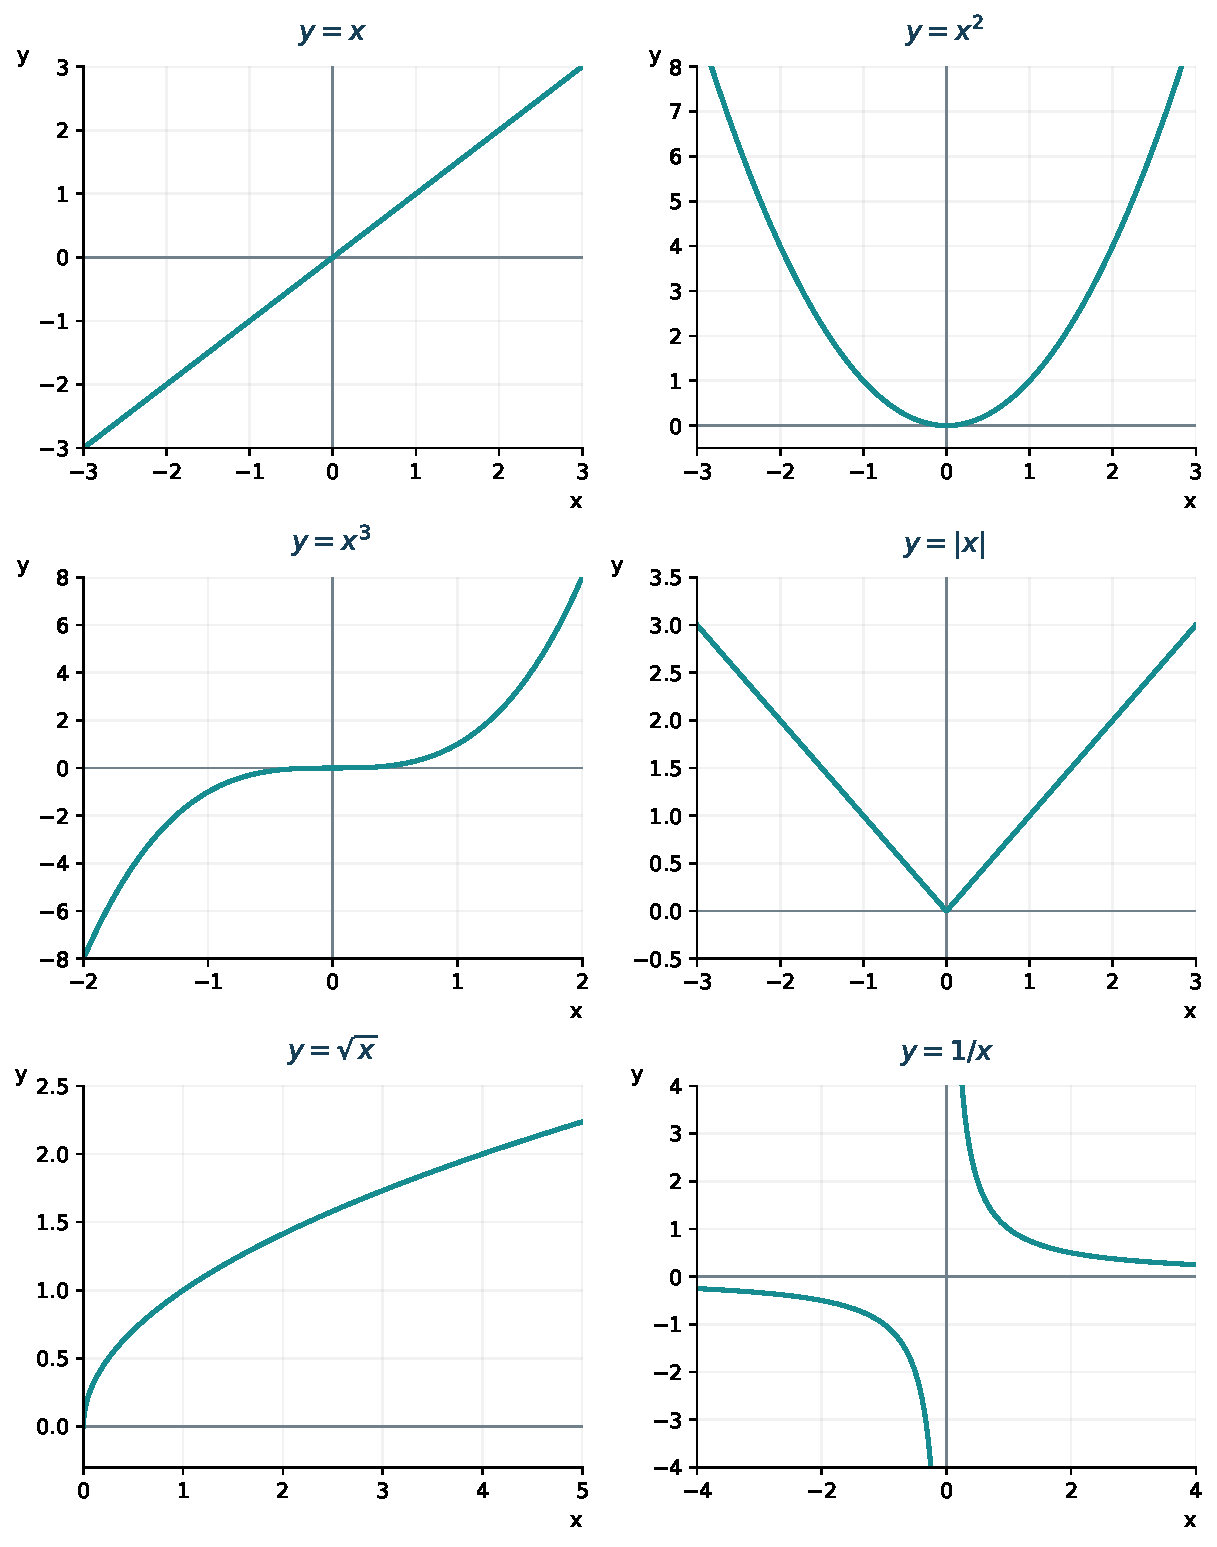
\includegraphics[width=\textwidth,height=.70\textheight,keepaspectratio]{images/atlas-algebra.pdf}\par\small Базовые алгебраические функции\end{center}\end{minipage}\par
\Needspace{7\baselineskip}\section*{Задачи}
\begingroup\setlength{\parskip}{3pt}
\noindent\begin{minipage}[t]{\linewidth}\textbf{13.1.} Для \(f (x) = 2 x - 3\) найди \(f (- 2),\allowbreak f (0),\allowbreak f (3)\).\par\end{minipage}\par
\noindent\begin{minipage}[t]{\linewidth}\textbf{13.2.} Найди область определения \(f (x) = \dfrac{1}{x - 4}\).\par\end{minipage}\par
\noindent\begin{minipage}[t]{\linewidth}\textbf{13.3.} Найди область определения \(f (x) = \sqrt{x + 3}\).\par\end{minipage}\par
\noindent\begin{minipage}[t]{\linewidth}\textbf{13.4.} Найди нули \(f (x) = x^{2} - 4\).\par\end{minipage}\par
\par\addvspace{5pt}\begin{lrbox}{\CatFlowBox}\begin{minipage}[t]{\linewidth}
\setlength{\parskip}{5pt}\setlength{\columnsep}{4.5mm}\setlength{\intextsep}{0pt}
\begin{wrapfigure}[12]{l}{54mm}

\includegraphics[width=54mm,height=58mm,keepaspectratio]{images/unique/art-38.png}
\end{wrapfigure}
\textbf{13.5.} Где \(f (x) = 3 x - 6\) положительна?\par

\textbf{13.6.} Построй \(y = 2 x + 1\) и найди пересечения с осями.\par

\textbf{13.7.} Построй \(y = (x - 2)^{2} - 1\). Укажи вершину.\par

\textbf{13.8.} Укажи промежутки убывания и возрастания \(y = x^{2}\).\par

\textbf{13.9.} Определи чётность \(f (x) = x^{3}\) и \(g (x) = x^{2} + 1\).\par

\textbf{13.10.} При \(f (x) = x^{2}\) и \(g (x) = x + 1\) найди \(f (g (x))\) и \(g (f (x))\).\par

\textbf{13.11.} Найди область значений \(y = (x - 1)^{2} + 2\).\par
\par\WFclear\end{minipage}\end{lrbox}%
\ifdim\dimexpr\ht\CatFlowBox+\dp\CatFlowBox\relax<64mm\dp\CatFlowBox=\dimexpr64mm-\ht\CatFlowBox\relax\fi%
\noindent\usebox{\CatFlowBox}\par\addvspace{5pt}

\noindent\begin{minipage}[t]{\linewidth}\textbf{13.12.} Найди точки пересечения \(y = x^{2}\) и \(y = x + 2\).\par\end{minipage}\par
\noindent\begin{minipage}[t]{\linewidth}\textbf{13.13.} Стоимость аренды велосипеда описана формулой \(C (t) = 200 + 150 t\) рублей, где \(t \ge  0\) — время в часах. Найди стоимость для \(0,\allowbreak 2\) и \(4\) часов и построй график.\par\end{minipage}\par
\noindent\begin{minipage}[t]{\linewidth}\textbf{13.14.} В баке \(60\) л воды. Её расходуют со скоростью \(5\) л в минуту, не доливая. Запиши объём \(V (t)\), укажи допустимое время и момент опустошения.\par\end{minipage}\par
\noindent\begin{minipage}[t]{\linewidth}\textbf{13.15.} Два тарифа доставки: \(A (x) = 100 + 20 x\) и \(B (x) = 40 x\) рублей, где \(x \ge  0\) — расстояние в километрах. При каком расстоянии цены равны? Какой тариф дешевле при \(2\) км и при \(8\) км?\par\end{minipage}\par
\noindent\begin{minipage}[t]{\linewidth}\textbf{13.16.}\starmark{} Найди область определения \(f (x) = \dfrac{\sqrt{x - 1}}{x - 3}\).\par\end{minipage}\par
\noindent\begin{minipage}[t]{\linewidth}\textbf{13.17.}\starmark{} Построй \(y = | x - 2 | + 1\) и найди все \(x\), для которых \(y \le  4\).\par\end{minipage}\par
\noindent\begin{minipage}[t]{\linewidth}\textbf{13.18.}\starmark{} Из куска проволоки длиной \(20\) м делают прямоугольник. Вырази площадь через сторону \(x\) и найди наибольшую площадь.\par\end{minipage}\par
\noindent\begin{minipage}[t]{\linewidth}\textbf{13.19.}\starmark{} Докажи, что при любых действительных \(a\ne0\) и \(b\) функция \(f(x)=ax+b\) задаёт биекцию \(\mathbb R\to\mathbb R\). Найди обратную функцию и проверь обе композиции.\par\end{minipage}\par
\noindent\begin{minipage}[t]{\linewidth}\textbf{13.20.}\starmark{} Пусть \(g:X\to Y\) и \(f:Y\to Z\) — инъекции. Докажи, что композиция \(f\circ g\) тоже инъективна. Затем докажи аналогичное утверждение для двух сюръекций.\par\end{minipage}\par
\noindent\begin{minipage}[t]{\linewidth}\textbf{13.21.} Построй график \(f(x)=|x|-2\). Найди область значений. Является ли отображение \(f:\mathbb R\to[-2;+\infty)\) инъекцией, сюръекцией, биекцией? Существует ли обратное отображение на всей указанной области?\par\end{minipage}\par
\noindent\begin{minipage}[t]{\linewidth}\textbf{13.22.}\starmark{} Для \(f(x)=\sqrt{x+1}+2\) найди область определения и область значений. Найди обратную функцию, указав её область определения. Построй оба графика в одной системе координат и проверь их симметрию относительно \(y=x\).\par\end{minipage}\par
\endgroup

\chapter{Комбинаторика и бином Ньютона}\label{chap:c10}\markright{Глава 14}
\section{Сначала определите, какие результаты считаются разными}

\begin{definition}
\term{Комбинаторика} (combinatorics) изучает способы выбора и расположения элементов,
а также число таких способов. При подсчёте нужно явно установить,
различаются ли элементы, важен ли порядок и разрешены ли повторения.
\end{definition}

Например, выбор капитана и его заместителя из Анны и Бориса имеет два результата:
капитан Анна и заместитель Борис либо наоборот.
Выбор команды из этих же двух человек имеет один результат.
В первом случае порядок ролей важен, во втором --- нет.
Если из букв \(A,B,C\) составляют двухбуквенную последовательность с повторениями,
то \(AA\) допустима; без повторений --- нет.

\section{Правила суммы и произведения}

\begin{theorem}[Правило суммы (sum rule)]\label{thm:legacy-c10-1}
Если первая группа содержит \(m\) различных результатов, вторая --- \(n\),
и эти группы не пересекаются, то выбрать один результат
из их объединения можно \(m+n\) способами.
\end{theorem}
\begin{proof}Перечислим сначала \(m\) результатов первой группы, затем \(n\) результатов второй. Группы не пересекаются, поэтому все перечисленные результаты различны и их ровно \(m+n\).\end{proof}

Например, если на полке \(5\) разных романов и \(3\) разных учебника,
одну книгу можно выбрать \(5+3=8\) способами.
Условие непересечения существенно: один результат нельзя посчитать дважды.

\Needspace{8\baselineskip}\begin{theorem}[Правило произведения (product rule)]\label{thm:legacy-c10-2}
Пусть выбор выполняется в несколько последовательных шагов.
Если на первом шаге есть \(n_1\) возможностей, после любого первого выбора
на втором есть ровно \(n_2\) возможностей, и так далее,
то полных последовательностей выборов ровно \(n_1n_2\cdots n_r\).
\end{theorem}
\par\addvspace{5pt}\begin{lrbox}{\CatFlowBox}\begin{minipage}[t]{\linewidth}
\setlength{\parskip}{5pt}\setlength{\columnsep}{4.5mm}\setlength{\intextsep}{0pt}
\begin{wrapfigure}[12]{l}{54mm}
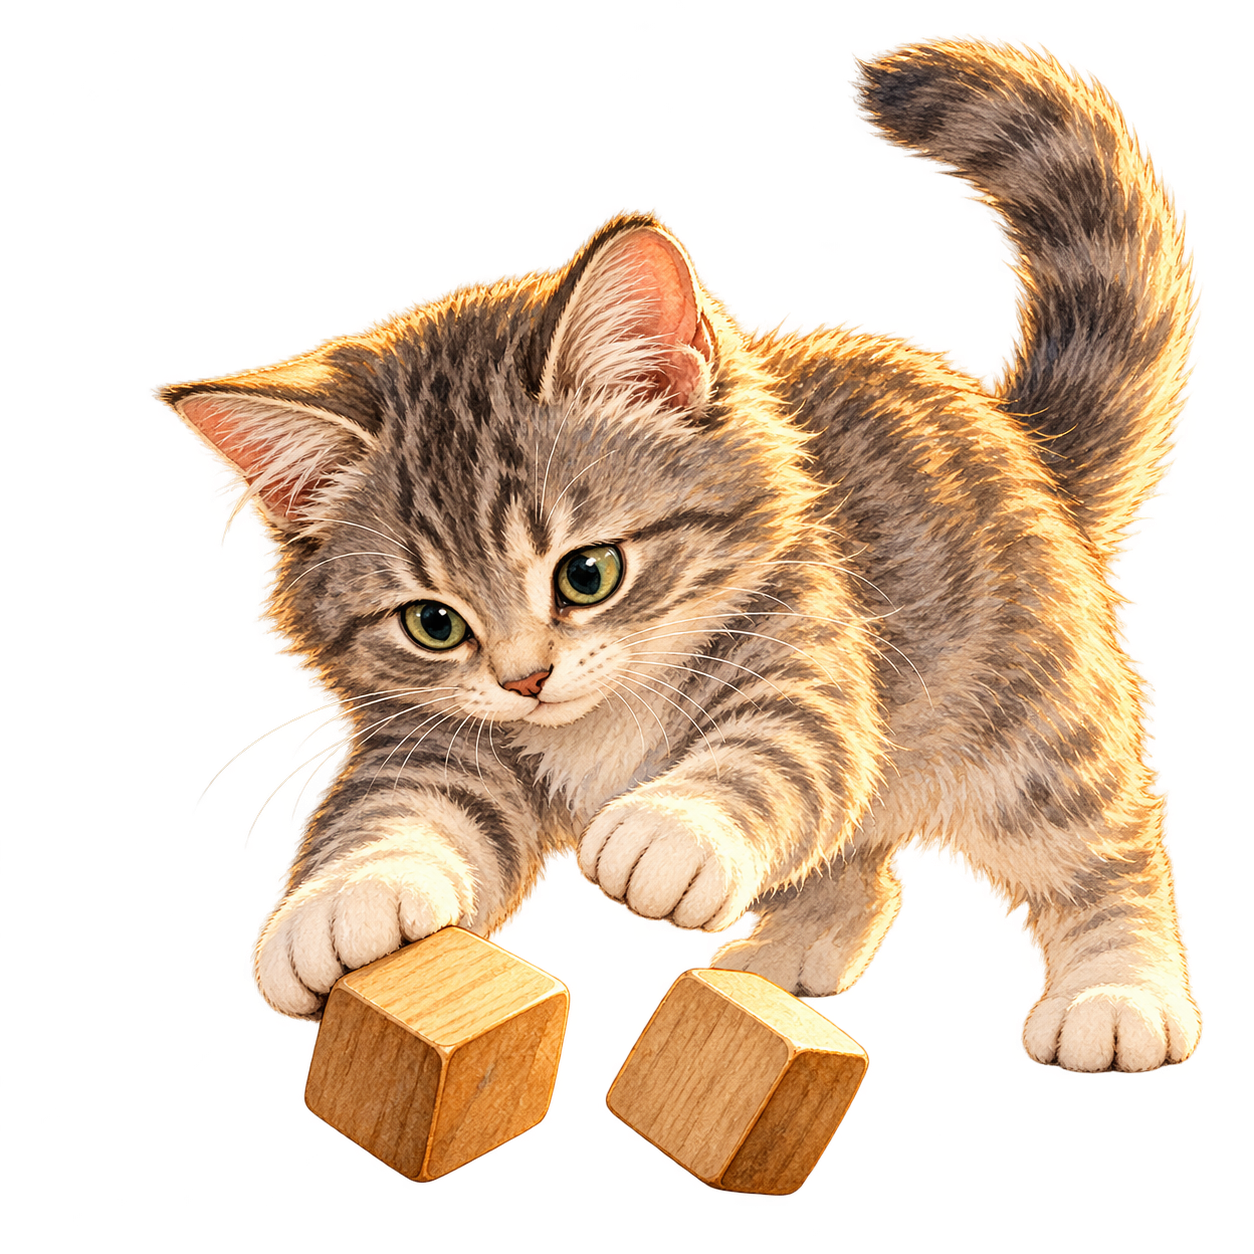
\includegraphics[width=54mm,height=58mm,keepaspectratio]{images/unique/art-17.png}
\end{wrapfigure}
\textit{Доказательство.} Для каждого результата первого шага имеется \(n_2\) продолжений. Получаются \(n_1\) непересекающихся групп по \(n_2\) исходов, всего \(n_1n_2\). Для большего числа шагов повторяем рассуждение, то есть применяем индукцию по числу шагов.\hfill\(\blacksquare\)

Например, к каждой из \(3\) рубашек можно надеть любые из \(2\) брюк:
получается \(3\cdot2=6\) комплектов.
Если число продолжений зависит от сделанного выбора, ветви сначала считают отдельно,
а затем складывают.
\par\WFclear\end{minipage}\end{lrbox}%
\ifdim\dimexpr\ht\CatFlowBox+\dp\CatFlowBox\relax<64mm\dp\CatFlowBox=\dimexpr64mm-\ht\CatFlowBox\relax\fi%
\noindent\usebox{\CatFlowBox}\par\addvspace{5pt}
\section{Факториал и перестановки}

\begin{definition}
\term{Факториал} (factorial) натурального числа \(n\) --- произведение всех натуральных чисел от \(1\) до \(n\):
\[
n!=1\cdot2\cdots n.
\]
Дополнительно полагают \(0!=1\). Поэтому для \(n\in\mathbb N_0\)
\[
(n+1)!=(n+1)n!.
\]
\end{definition}

Значение \(0!=1\) соответствует одному способу расположить ноль элементов:
получить пустую последовательность. Например, \(4!=24\).

\begin{definition}
\term{Перестановка без повторений} (permutation without repetition) ---
расположение всех \(n\) различных элементов в определённом порядке.
\end{definition}

На первое место есть \(n\) вариантов, на второе --- \(n-1\), и так далее.
По правилу произведения число перестановок равно
\[
P_n=n!.
\]

\begin{definition}
\term{Перестановка с повторениями} (multiset permutation) ---
расположение \(n\) элементов, среди которых есть одинаковые:
\(n_1\) элементов первого вида, \(n_2\) второго и так далее,
где \(n_1+\cdots+n_r=n\).
\end{definition}

Число таких перестановок равно
\[
P(n_1,\ldots,n_r)=\frac{n!}{n_1!\cdots n_r!}.
\]
Действительно, если временно различить все одинаковые элементы,
каждое конечное расположение будет учтено \(n_1!\cdots n_r!\) раз.
Например, из букв слова «МАМА» получается \(\frac{4!}{2!2!}=6\) разных последовательностей.

\section{Размещения: порядок важен}

\begin{definition}
\term{Размещение без повторений} (ordered selection without repetition) ---
упорядоченный выбор \(k\) различных элементов из \(n\) различных элементов.
\end{definition}

Для \(0\le k\le n\) число размещений равно
\[
A_n^k=\frac{n!}{(n-k)!}.
\]
При \(k\ge1\) это произведение \(k\) множителей:
\(n(n-1)\cdots(n-k+1)\); при \(k=0\) имеется один пустой выбор.
Например, капитана и заместителя из \(5\) человек выбирают \(A_5^2=5\cdot4=20\) способами.

\begin{definition}
\term{Размещение с повторениями} (ordered selection with repetition) ---
последовательность длины \(k\), каждый элемент которой выбирают из \(n\) видов;
один и тот же вид можно выбирать несколько раз.
\end{definition}

При \(n\ge1\), \(k\in\mathbb N_0\) число таких последовательностей равно
\[
\overline A_n^k=n^k.
\]
Например, двухсимвольных кодов из букв \(A,B,C\) ровно \(3^2=9\):
\(AA,AB,AC,BA,BB,BC,CA,CB,CC\).

\section{Сочетания: порядок не важен}

\begin{definition}
\term{Сочетание без повторений} (combination without repetition) ---
выбор \(k\) элементов из \(n\) различных элементов, при котором порядок не учитывается
и каждый элемент выбирают не более одного раза.
\end{definition}

Каждый такой выбор порождает \(k!\) размещений, поэтому
\[
C_n^k=\binom nk=\frac{n!}{k!(n-k)!},\qquad 0\le k\le n.
\]
Например, пару участников из \(5\) человек выбирают \(\binom52=10\) способами.
Здесь обмен участников местами не создаёт новую пару.

\begin{definition}
\term{Сочетание с повторениями} (combination with repetition) ---
выбор \(k\) элементов из \(n\) видов, при котором порядок не учитывается,
а элементы каждого вида можно брать в любом количестве.
\end{definition}

При \(n\ge1\), \(k\in\mathbb N_0\) число таких выборов равно
\[
\overline C_n^k=\binom{n+k-1}{k}=\binom{n+k-1}{n-1}.
\]
Выбор задаётся количествами \(x_1,\ldots,x_n\) элементов каждого вида:
\(x_i\in\mathbb N_0\), \(x_1+\cdots+x_n=k\).
Чтобы увидеть формулу, расположим в строку \(k\) одинаковых звёздочек и \(n-1\) перегородок.
Количество звёздочек до первой перегородки задаёт \(x_1\), между первой и второй --- \(x_2\), и так далее.
Перегородки могут стоять рядом и по краям: это соответствует нулевым количествам.
Нужно выбрать позиции \(n-1\) перегородок среди \(n+k-1\) позиций.
Например, для \(3\) видов и \(4\) элементов получается \(\binom62=15\) выборов.

\section{Биномиальные коэффициенты}

\begin{definition}
\term{Биномиальный коэффициент} (binomial coefficient) \(\binom nk\)
--- число сочетаний без повторений из \(n\) элементов по \(k\).
\end{definition}

Непосредственно из смысла выбора следуют равенства
\[
\binom n0=\binom nn=1,\qquad
\binom nk=\binom n{n-k}.
\]
Последнее равенство выражает соответствие между выбранными \(k\) элементами
и \(n-k\) оставшимися.

\begin{theorem}[Тождество Паскаля (Pascal's identity)]\label{thm:legacy-c10-3}
Для целых \(n\ge1\), \(1\le k\le n\)
\[
\binom{n+1}k=\binom n{k-1}+\binom nk.
\]
\end{theorem}

\begin{proof}
Выделим один элемент из \(n+1\) различных элементов.
Если он входит в выбранную группу из \(k\) элементов,
остальных участников выбирают \(\binom n{k-1}\) способами.
Если не входит, всю группу выбирают \(\binom nk\) способами.
Эти случаи не пересекаются и охватывают все группы; применяем правило суммы.
\end{proof}

\section{Бином Ньютона}

\begin{theorem}[Бином Ньютона (binomial theorem)]\label{thm:legacy-c10-4}
Для любых рациональных чисел \(a,b\) и любого натурального \(n\)
\[
(a+b)^n=a^n+\sum_{k=1}^{n-1}\binom nk a^{n-k}b^k+b^n.
\]
Знак \(\sum\) означает сложение слагаемых при всех указанных значениях индекса \(k\).
При \(n=1\) внутренняя сумма пуста и равна нулю, так что формула даёт \(a+b=a+b\).
\end{theorem}

\par\addvspace{5pt}\begin{lrbox}{\CatFlowBox}\begin{minipage}[t]{\linewidth}
\setlength{\parskip}{5pt}\setlength{\columnsep}{4.5mm}\setlength{\intextsep}{0pt}
\begin{wrapfigure}[12]{r}{54mm}

\includegraphics[width=54mm,height=58mm,keepaspectratio]{images/unique/art-18.png}
\end{wrapfigure}
\textit{Доказательство.} Раскроем произведение \(n\) одинаковых скобок \((a+b)\).
В каждом слагаемом из каждой скобки выбран либо \(a\), либо \(b\).
Если при \(1\le k\le n-1\) число \(b\) выбрано ровно из \(k\) скобок,
а \(a\) --- из остальных, получается \(a^{n-k}b^k\).
Нужные \(k\) скобок можно выбрать \(\binom nk\) способами.
Выбор только \(a\) даёт \(a^n\), выбор только \(b\) --- \(b^n\).
Собирая одинаковые слагаемые, получаем формулу.\hfill\(\blacksquare\)
\par\WFclear\end{minipage}\end{lrbox}%
\ifdim\dimexpr\ht\CatFlowBox+\dp\CatFlowBox\relax<64mm\dp\CatFlowBox=\dimexpr64mm-\ht\CatFlowBox\relax\fi%
\noindent\usebox{\CatFlowBox}\par\addvspace{5pt}


Например,
\[
(a+b)^3=a^3+3a^2b+3ab^2+b^3.
\]
Запись с отдельно выписанными крайними слагаемыми позволяет применять формулу
и при \(a=0\) или \(b=0\), не вводя выражение \(0^0\).

\section{Примеры: порядок выбора и коэффициент бинома}
\begin{example}Из восьми человек выбирают двух дежурных с одинаковыми обязанностями: \(C_8^2=28\). Если выбирают старосту и заместителя, роли различны: \(8\cdot7=56\). Каждой неупорядоченной паре соответствуют два распределения ролей. Возвращение одного человека в выбор здесь не разрешено.\end{example}
\begin{example}Коэффициент при \(x^2\) в \((1+2x)^4\) равен \(C_4^2\cdot2^2=24\): выбираем ровно два множителя, из которых берём \(2x\), из остальных берём единицу. Член бинома Ньютона имеет вид \(C_4^k(2x)^k\), поэтому степень аргумента определяет индекс \(k\).\end{example}
\Needspace{7\baselineskip}\section*{Задачи}
\begingroup\setlength{\parskip}{2pt}
\noindent\begin{minipage}[t]{\linewidth}\textbf{14.1.} На полке стоят \(5\) разных романов и \(3\) разных учебника. Сколько есть способов выбрать одну книгу?\par\end{minipage}\par
\noindent\begin{minipage}[t]{\linewidth}\textbf{14.2.} Есть \(4\) рубашки, \(3\) пары брюк и \(2\) пары обуви. Любые вещи можно сочетать. Сколько комплектов из одной рубашки, одной пары брюк и одной пары обуви можно составить?\par\end{minipage}\par
\noindent\begin{minipage}[t]{\linewidth}\textbf{14.3.} Для каждого выбора укажи, важен ли порядок и разрешены ли повторения: а) распределить три призовых места между \(10\) участниками без ничьих; б) выбрать команду из \(3\) человек среди \(10\); в) составить код длины \(3\) из цифр \(0,\ldots,9\), допуская одинаковые цифры; г) выбрать \(3\) элемента из \(4\) видов, допуская один вид несколько раз и не учитывая порядок.\par\end{minipage}\par
\noindent\begin{minipage}[t]{\linewidth}\textbf{14.4.} Вычисли \(5!\), \(0!\) и \(\dfrac{7!}{5!}\).\par\end{minipage}\par
\noindent\begin{minipage}[t]{\linewidth}\textbf{14.5.} Сколькими способами можно расположить в ряд \(6\) различных книг, используя каждую ровно один раз?\par\end{minipage}\par
\noindent\begin{minipage}[t]{\linewidth}\textbf{14.6.} Сколько разных последовательностей можно получить, переставляя все буквы слова «ТОПОТ»? Осмысленность полученных слов не требуется.\par\end{minipage}\par
\noindent\begin{minipage}[t]{\linewidth}\textbf{14.7.} В забеге участвуют \(8\) человек. Сколько существует вариантов распределения первого, второго и третьего мест, если ничьи невозможны?\par\end{minipage}\par
\noindent\begin{minipage}[t]{\linewidth}\textbf{14.8.} Из \(8\) различных элементов выбирают \(3\), не учитывая порядок. Сколько существует выборов?\par\end{minipage}\par
\noindent\begin{minipage}[t]{\linewidth}\textbf{14.9.} Электронный замок принимает код из \(4\) цифр от \(0\) до \(9\). Повторения разрешены, первая цифра может быть нулём. Сколько разных кодов возможно?\par\end{minipage}\par
\noindent\begin{minipage}[t]{\linewidth}\textbf{14.10.} Сколько существует четырёхзначных натуральных чисел с попарно различными цифрами?\par\end{minipage}\par
\noindent\begin{minipage}[t]{\linewidth}\textbf{14.11.} Из \(4\) видов элементов выбирают \(3\) элемента. Каждый вид можно использовать сколько угодно раз, порядок не учитывается. Сколько существует выборов?\par\end{minipage}\par
\noindent\begin{minipage}[t]{\linewidth}\textbf{14.12.} Сколькими способами можно разложить \(7\) одинаковых шаров по \(3\) различным ящикам? Пустые ящики допускаются.\par\end{minipage}\par
\noindent\begin{minipage}[t]{\linewidth}\textbf{14.13.} Из множества, состоящего из \(n\ge2\) элементов, можно выбрать ровно \(45\) различных неупорядоченных пар. Найди \(n\).\par\end{minipage}\par
\par\addvspace{5pt}\begin{lrbox}{\CatFlowBox}\begin{minipage}[t]{\linewidth}
\setlength{\parskip}{5pt}\setlength{\columnsep}{4.5mm}\setlength{\intextsep}{0pt}
\begin{wrapfigure}[12]{l}{54mm}

\includegraphics[width=54mm,height=58mm,keepaspectratio]{images/unique/art-29.png}
\end{wrapfigure}
\textbf{14.14.} Пользуясь тождеством Паскаля и значениями \(\binom72=21\), \(\binom73=35\), вычисли \(\binom83\).\par

\textbf{14.15.} Раскрой скобки в \((x+2)^4\) с помощью бинома Ньютона.\par

\textbf{14.16.} Найди коэффициент при \(x^3\) после раскрытия скобок в \((2+x)^7\).\par

\textbf{14.17.} Докажи, что для любого \(n\in\mathbb N_0\) выполняется \(\sum_{k=0}^{n}\binom nk=2^n\).\par

\textbf{14.18.}\starmark{} Из \(4\) девушек и \(6\) юношей выбирают группу из \(5\) человек. Сколько существует групп, в которых не меньше двух девушек?\par

\textbf{14.19.}\starmark{} Сколько кодов длины \(5\) из цифр \(0,\ldots,9\) содержат хотя бы один ноль и хотя бы одну единицу? Начальный ноль разрешён, повторения разрешены.\par

\textbf{14.20.}\starmark{} Докажи подсчётом одного и того же множества двумя способами тождество Вандермонда: \(\sum_{k=0}^{r}\binom mk\binom n{r-k}=\binom{m+n}{r}\), где \(m,n\in\mathbb N_0\), \(0\le r\le m+n\). В этой задаче \(\binom uv=0\), если целое \(v<0\) или \(v>u\). Рассматривай целое \(r\in\mathbb N_0\).\par
\par\WFclear\end{minipage}\end{lrbox}%
\ifdim\dimexpr\ht\CatFlowBox+\dp\CatFlowBox\relax<64mm\dp\CatFlowBox=\dimexpr64mm-\ht\CatFlowBox\relax\fi%
\noindent\usebox{\CatFlowBox}\par\addvspace{5pt}

\endgroup

\chapter{Тригонометрия}
\begin{definition}\term{Радиан} (\emph{radian}) — единица измерения угла. Угол в \(1\) радиан — центральный угол, которому соответствует дуга длины, равной радиусу окружности. Радианная мера центрального угла равна \(\alpha=\frac{l}{r}\), где \(l\) — длина дуги, \(r>0\) — радиус. Полный оборот: \(2\pi\) радиан, то есть \(360^\circ\).\end{definition}
Положительные углы отсчитывают от точки \((1;0)\) единичной окружности против часовой стрелки, отрицательные — по часовой.
\begin{definition}\term{Косинус} (\emph{cosine}) \(\cos\alpha\) — горизонтальная координата точки единичной окружности, полученной поворотом точки \((1;0)\) на угол \(\alpha\).\end{definition}
\begin{definition}\term{Синус} (\emph{sine}) \(\sin\alpha\) — вертикальная координата точки единичной окружности, полученной поворотом точки \((1;0)\) на угол \(\alpha\).\end{definition}
\begin{definition}\term{Тангенс} (\emph{tangent}): \(\tan  \alpha  = \frac{\sin  \alpha }{\cos  \alpha }\) при \(\cos  \alpha  \ne  0\).\end{definition}
\begin{definition}\term{Период функции} (\emph{period of a function}) — ненулевое число \(T\), при сдвиге аргумента на которое область определения сохраняется и \(f (x + T) = f (x)\).\end{definition}
\section*{Основные тождества и свойства}
\(\sin ^{2} \alpha  + \cos ^{2} \alpha  = 1\). Значения синуса и косинуса лежат в \([- 1;\allowbreak 1]\).\par
\(\sin  (- \alpha ) = - \sin  \alpha ;\allowbreak \cos  (- \alpha ) = \cos  \alpha \).\par
\(\sin  (\pi  - \alpha ) = \sin  \alpha ;\allowbreak \cos  (\pi  - \alpha ) = - \cos  \alpha \).\par
Наименьший положительный период синуса и косинуса равен \(2 \pi \). Для \(\sin  (kx)\) и \(\cos  (kx)\) при \(k \ne  0\) он равен \(\frac{2 \pi }{| k |}\).\par
\section*{Прямоугольный треугольник}
Для острого угла синус — \(\frac{\text{противолежащий катет}}{\text{гипотенуза}}\); косинус — \(\frac{\text{прилежащий катет}}{\text{гипотенуза}}\); тангенс — \(\frac{\text{противолежащий катет}}{\text{прилежащий катет}}\).\par
\section*{Значения, которые стоит знать}
\(\sin  0 = 0;\allowbreak \sin  (\frac{\pi }{6}) = \frac{1}{2};\allowbreak \sin  (\frac{\pi }{4}) = \frac{\sqrt{2}}{2};\allowbreak \sin  (\frac{\pi }{3}) = \frac{\sqrt{3}}{2};\allowbreak \sin  (\frac{\pi }{2}) = 1\).\par
\(\cos  0 = 1;\allowbreak \cos  (\frac{\pi }{6}) = \frac{\sqrt{3}}{2};\allowbreak \cos  (\frac{\pi }{4}) = \frac{\sqrt{2}}{2};\allowbreak \cos  (\frac{\pi }{3}) = \frac{1}{2};\allowbreak \cos  (\frac{\pi }{2}) = 0\).\par
{\small\textit{Пример: \(60 {}^{\circ} = \frac{\pi }{3}\) радиан, потому что \(60 \cdot  \frac{\pi }{180} = \frac{\pi }{3}\).}}\par

\section*{Обратные тригонометрические функции}
На всей числовой прямой синус и косинус принимают одни и те же значения много раз. Чтобы получить обратную функцию, нужно выбрать промежуток, на котором каждому значению соответствует ровно один аргумент.
\begin{definition}\term{Арксинус} (arcsine) \(\arcsin t\) — единственный угол \(\alpha\in[-\frac\pi2;\frac\pi2]\), для которого \(\sin\alpha=t\). Область определения: \(t\in[-1;1]\); область значений: \([-\frac\pi2;\frac\pi2]\).\end{definition}
\begin{definition}\term{Арккосинус} (arccosine) \(\arccos t\) — единственный угол \(\alpha\in[0;\pi]\), для которого \(\cos\alpha=t\). Область определения: \(t\in[-1;1]\); область значений: \([0;\pi]\).\end{definition}
\begin{definition}\term{Арктангенс} (arctangent) \(\arctan t\) — единственный угол \(\alpha\in(-\frac\pi2;\frac\pi2)\), для которого \(\tan\alpha=t\). Область определения: \(t\in\mathbb R\); область значений: \((-\frac\pi2;\frac\pi2)\).\end{definition}
Синус на \([-\frac\pi2;\frac\pi2]\) и тангенс на \((-\frac\pi2;\frac\pi2)\) строго возрастают, а косинус на \([0;\pi]\) строго убывает. Именно эти ограничения позволяют определить обратные функции. Их графики получают отражением соответствующих ограниченных графиков относительно \(y=x\).
По определениям \(\sin(\arcsin t)=t\), \(\cos(\arccos t)=t\) при \(t\in[-1;1]\), а \(\tan(\arctan t)=t\) при всех действительных \(t\). Обратный порядок требует ограничения аргумента: \(\arcsin(\sin x)=x\) только при \(x\in[-\frac\pi2;\frac\pi2]\); \(\arccos(\cos x)=x\) только при \(x\in[0;\pi]\); \(\arctan(\tan x)=x\) только при \(x\in(-\frac\pi2;\frac\pi2)\). Вне этих промежутков результат нужно привести к области значений обратной функции. В частности, \(\arcsin(\sin\frac{5\pi}6)=\arcsin\frac12=\frac\pi6\), а не \(\frac{5\pi}6\). При \(x=\frac\pi2+\pi k\), \(k\in\mathbb Z\), сама запись \(\arctan(\tan x)\) не определена.
\begin{theorem}[Связь арксинуса и арккосинуса]
Для любого \(t\in[-1;1]\) выполнено \(\arcsin t+\arccos t=\frac\pi2\).
\end{theorem}
\begin{proof}
Пусть \(\alpha=\arcsin t\); тогда \(\alpha\in[-\frac\pi2;\frac\pi2]\) и \(\sin\alpha=t\). Угол \(\beta=\frac\pi2-\alpha\) принадлежит \([0;\pi]\), а \(\cos\beta=\sin\alpha=t\). По единственности угла в определении арккосинуса \(\beta=\arccos t\), откуда следует нужное равенство.
\end{proof}
В некоторых источниках обозначения \(\sin^{-1}t\), \(\cos^{-1}t\), \(\tan^{-1}t\) означают обратные функции. Чтобы не путать их с обратными числами \(\frac1{\sin t}\), \(\frac1{\cos t}\), \(\frac1{\tan t}\), здесь используем только записи \(\arcsin\), \(\arccos\), \(\arctan\).

\clearpage\section*{Графики}
\begin{center}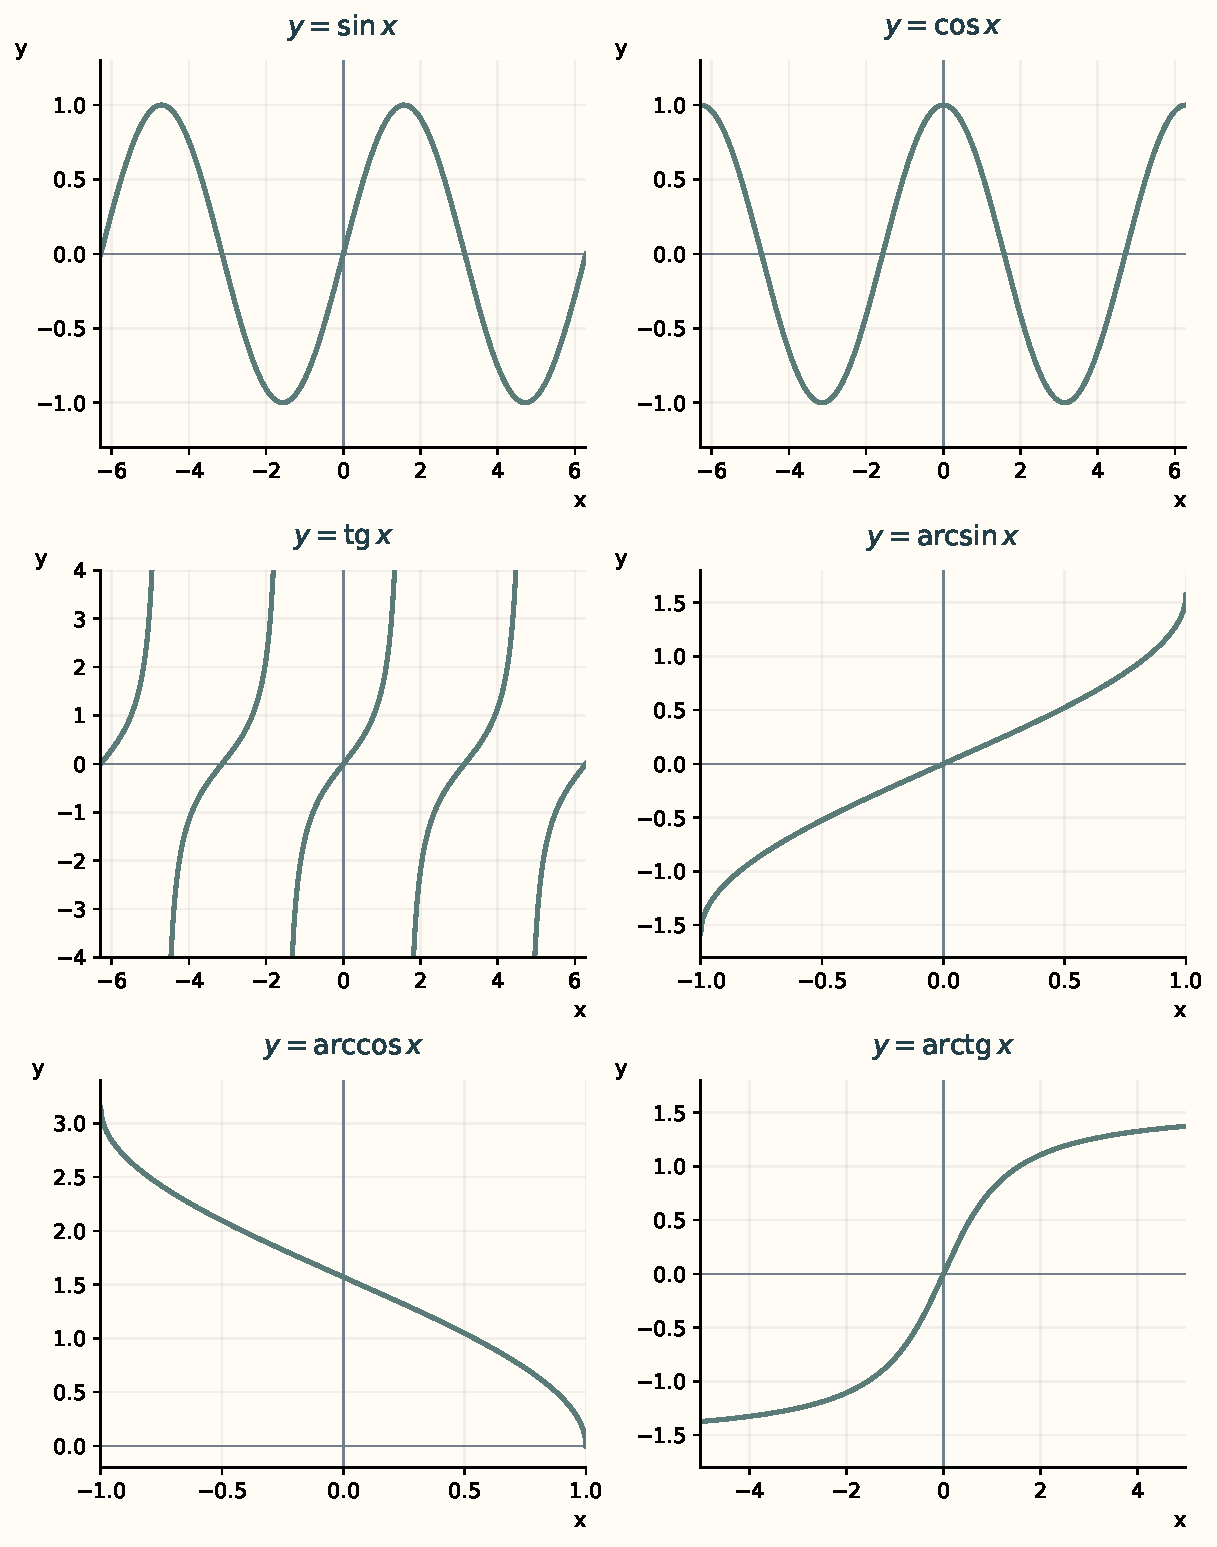
\includegraphics[width=\textwidth,height=.79\textheight,keepaspectratio]{images/atlas-trigonometry.pdf}\par\small Тригонометрические и обратные функции\end{center}
\Needspace{7\baselineskip}\section*{Задачи}
\begin{enumerate}[label={},leftmargin=3.2em,itemsep=10pt]
\Needspace{3\baselineskip}\item[\textbf{15.1.}] Переведи \(30 {}^{\circ},\allowbreak 90 {}^{\circ}\) и \(150 {}^{\circ}\) в радианы.
\Needspace{3\baselineskip}\item[\textbf{15.2.}] Переведи \(\frac{\pi }{4}\) и \(\frac{7 \pi }{6}\) в градусы.
\Needspace{3\baselineskip}\item[\textbf{15.3.}] Вычисли \(\sin  (\frac{\pi }{6}),\allowbreak \cos  (\frac{\pi }{3}),\allowbreak \tan  (\frac{\pi }{4})\).
\Needspace{3\baselineskip}\item[\textbf{15.4.}] Определи знаки \(\sin \) и \(\cos \) для угла \(\frac{5 \pi }{6}\).
\Needspace{3\baselineskip}\item[\textbf{15.5.}] Найди \(\sin  (- \frac{\pi }{6})\) и \(\cos  (- \frac{\pi }{3})\).
\Needspace{3\baselineskip}\item[\textbf{15.6.}] Упрости \(\sin ^{2} x + \cos ^{2} x + 2\).
\Needspace{3\baselineskip}\item[\textbf{15.7.}] Если \(\sin  x = \frac{3}{5}\) и \(0 < x < \frac{\pi }{2}\), найди \(\cos  x\) и \(\tan  x\).
\Needspace{3\baselineskip}\item[\textbf{15.8.}] Найди \(\sin  (\pi  - x)\) и \(\cos  (\pi  - x)\) через функции \(x\).
\Needspace{3\baselineskip}\item[\textbf{15.9.}] Реши \(\sin  x = 0\) при \(x \in  [0;\allowbreak 2 \pi ]\).
\Needspace{3\baselineskip}\item[\textbf{15.10.}] Реши \(\cos  x = \frac{1}{2}\) при \(x \in  [0;\allowbreak 2 \pi ]\).
\Needspace{3\baselineskip}\item[\textbf{15.11.}] Построй \(y = \sin  x\) на \([0;\allowbreak 2 \pi ]\). Укажи нули, максимум и минимум.
\Needspace{3\baselineskip}\item[\textbf{15.12.}] Найди наименьший положительный период \(y = \sin  (2 x)\).
\Needspace{3\baselineskip}\item[\textbf{15.13.}] Из жизни. Солнечный луч образует с землёй угол \(45 {}^{\circ}\). Тень вертикального столба равна \(6\) м. Найди высоту столба.
\Needspace{3\baselineskip}\item[\textbf{15.14.}] Из жизни. Лестница длиной \(10\) м образует с горизонтальной землёй угол \(30 {}^{\circ}\). На какой высоте находится её верх?
\Needspace{3\baselineskip}\item[\textbf{15.15.}] Из жизни. Колесо обозрения радиусом \(10\) м имеет центр на высоте \(12\) м. Высота кабинки \(h = 12 + 10 \sin  \alpha \). Найди высоту при \(\alpha  = 0,\allowbreak \frac{\pi }{2}\) и \(\frac{3 \pi }{2}\).
\Needspace{3\baselineskip}\item[\textbf{15.16.}\starmark] Реши \(2 \sin ^{2} x - 3 \sin  x + 1 = 0\) при \(x \in  [0;\allowbreak 2 \pi ]\).
\Needspace{3\baselineskip}\item[\textbf{15.17.}\starmark] Луч образует с землёй угол \(30 {}^{\circ}\). Длина тени вертикального дерева \(12\) м. Найди высоту дерева в точном виде.
\Needspace{3\baselineskip}\item[\textbf{15.18.}\starmark] Высота кабинки задана \(h (t) = 15 - 12 \cos  (\frac{\pi  t}{20})\) метров, где \(t\) — секунды от начала движения. Найди минимальную и максимальную высоты и время первого достижения максимума при \(t \ge  0\).
\begin{center}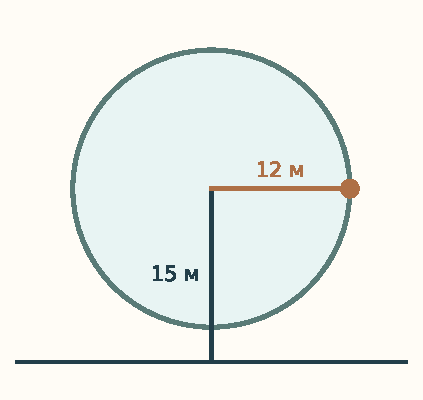
\includegraphics[width=.7\linewidth,height=45mm,keepaspectratio]{images/diagram-wheel.pdf}\end{center}
\Needspace{3\baselineskip}\item[\textbf{15.19.}\starmark] Докажи нечётность арксинуса: \(\arcsin(-t)=-\arcsin t\) для \(t\in[-1;1]\). В доказательстве проверь область значений угла, а не только равенство синусов.
\Needspace{3\baselineskip}\item[\textbf{15.20.}\starmark] Докажи тождество \(\arccos(-t)=\pi-\arccos t\) при \(t\in[-1;1]\).
\Needspace{3\baselineskip}\item[\textbf{15.21.}] Вычисли \(\arcsin0\), \(\arcsin\frac12\), \(\arcsin(-\frac{\sqrt3}{2})\).
\Needspace{3\baselineskip}\item[\textbf{15.22.}] Вычисли \(\arccos(-\frac12)\), \(\arccos1\), \(\arccos0\).
\Needspace{3\baselineskip}\item[\textbf{15.23.}] Вычисли \(\arctan(-1)\), \(\arctan\sqrt3\), \(\arctan0\).
\Needspace{3\baselineskip}\item[\textbf{15.24.}\starmark] Вычисли \(\arcsin(\sin\frac{5\pi}6)\), \(\arccos(\cos\frac{5\pi}3)\), \(\arctan(\tan\frac{3\pi}4)\). Для каждого ответа проверь диапазон обратной функции.
\Needspace{3\baselineskip}\item[\textbf{15.25.}] Найди \(\cos(\arcsin\frac35)\) и \(\sin(\arccos(-\frac35))\). Обоснуй выбор знака квадратного корня.
\Needspace{3\baselineskip}\item[\textbf{15.26.}] Реши \(\arcsin(2x-1)=\frac\pi6\). Сначала найди область допустимых значений.
\Needspace{3\baselineskip}\item[\textbf{15.27.}] Реши \(\arctan(x-2)=-\frac\pi4\).
\Needspace{3\baselineskip}\item[\textbf{15.28.}] Построй эскиз \(y=\arctan x\), отметив точки с аргументами \(-1\), \(0\), \(1\). Укажи область определения, область значений и чётность. Может ли значение функции быть равным \(\frac\pi2\)?
\end{enumerate}

\chapter{Множества, логика и доказательства}\markright{Глава 16}
\begin{definition}\term{Множество} (\emph{set}) — совокупность элементов. Запись \(x \in  A\) означает, что \(x\) принадлежит множеству \(A\).\end{definition}
\begin{definition}\term{Пересечение} (\emph{intersection}) \(A\cap B\) — множество элементов, принадлежащих одновременно \(A\) и \(B\).\end{definition}
\begin{definition}\term{Объединение} (\emph{union}) \(A\cup B\) — множество элементов, принадлежащих хотя бы одному из множеств \(A\) и \(B\).\end{definition}
\begin{definition}\term{Утверждение} (\emph{statement; proposition}) — высказывание, для которого можно определить истинность или ложность в заданных условиях.\end{definition}
\begin{definition}\term{Импликация} (\emph{implication}) \(P\Rightarrow Q\) — высказывание «если \(P\), то \(Q\)».\end{definition}
\begin{definition}\term{Достаточное условие} (\emph{sufficient condition}) для \(Q\) — условие \(P\), из которого следует \(Q\), то есть импликация \(P\Rightarrow Q\) истинна.\end{definition}
\begin{definition}\term{Необходимое условие} (\emph{necessary condition}) для \(P\) — условие \(Q\), которое обязательно выполняется при выполнении \(P\), то есть импликация \(P\Rightarrow Q\) истинна.\end{definition}
\section*{Кванторы и отрицание}
\par\addvspace{5pt}\begin{lrbox}{\CatFlowBox}\begin{minipage}[t]{\linewidth}
\setlength{\parskip}{5pt}\setlength{\columnsep}{4.5mm}\setlength{\intextsep}{0pt}
\begin{wrapfigure}[12]{r}{54mm}

\includegraphics[width=54mm,height=58mm,keepaspectratio]{images/unique/art-23.png}
\end{wrapfigure}
\(\forall \) означает «для любого», \(\exists \) — «существует». \(\mathbb{Z}\) обозначает целые числа, \(\mathbb{R}\) — действительные.\par
Отрицание «для всех \(x\) верно \(P (x)\)» — «существует \(x\), для которого \(P (x)\) неверно».\par
Чтобы опровергнуть всеобщее утверждение, достаточно одного контрпримера. Чтобы доказать его, проверки нескольких примеров недостаточно.\par
\par\WFclear\end{minipage}\end{lrbox}%
\ifdim\dimexpr\ht\CatFlowBox+\dp\CatFlowBox\relax<64mm\dp\CatFlowBox=\dimexpr64mm-\ht\CatFlowBox\relax\fi%
\noindent\usebox{\CatFlowBox}\par\addvspace{5pt}
\section*{Свойства и способы доказательства}
Для конечных множеств: \(| A \cup  B | = | A | + | B | - | A \cap  B |\). Здесь \(| A |\) означает число элементов множества, а не модуль числа.\par
\begin{definition}\term{Контрапозиция} (\emph{contrapositive}) импликации \(P\Rightarrow Q\) — импликация \(\neg Q\Rightarrow\neg P\), равносильная исходной:\[ (P\Rightarrow Q)\Longleftrightarrow(\neg Q\Rightarrow\neg P). \] Здесь \(\neg\) означает отрицание.\end{definition}
Обратное утверждение \(Q\Rightarrow P\) в общем случае из \(P\Rightarrow Q\) не следует.\par
Принцип математической индукции: проверь утверждение для \(n = 1\); затем для любого \(k \ge  1\) докажи переход от его истинности при \(n = k\) к истинности при \(n = k + 1\). Тогда оно верно для всех натуральных \(n \ge  1\).\par
{\small\textit{Пример прямого доказательства: сумма чётных чисел \(2 m\) и \(2 n\) равна \(2 (m + n)\), поэтому она чётна.}}\par

\section*{Подмножества и операции над множествами}
\begin{definition}\term{Подмножество} (subset) \(A\) множества \(B\) — множество, каждый элемент которого принадлежит \(B\). Обозначение \(A\subseteq B\) допускает равенство \(A=B\).\end{definition}
\begin{definition}\term{Собственное подмножество} (proper subset) — подмножество \(A\subseteq B\), не равное \(B\). Обозначение: \(A\subsetneq B\).\end{definition}
\begin{definition}\term{Пустое множество} (empty set) \(\varnothing\) — множество, не содержащее ни одного элемента. Оно является подмножеством любого множества; \(\{\varnothing\}\) содержит один элемент и не равно \(\varnothing\).\end{definition}
\begin{definition}\term{Универсальное множество} (universal set) \(U\) — заранее выбранное множество всех объектов, рассматриваемых в данной задаче. Если говорится о дополнениях, все обсуждаемые множества считаются подмножествами \(U\).\end{definition}
\begin{definition}\term{Разность множеств} (set difference) \(A\setminus B\) — множество элементов, которые принадлежат \(A\), но не принадлежат \(B\).\end{definition}
\begin{definition}\term{Дополнение множества} (complement) \(A\subseteq U\) относительно \(U\) — множество \(U\setminus A\). Без указания \(U\) дополнение может быть неоднозначным.\end{definition}
\begin{definition}\term{Симметрическая разность} (symmetric difference) \(A\triangle B\) — множество элементов, принадлежащих ровно одному из множеств \(A,B\): \(A\triangle B=(A\setminus B)\cup(B\setminus A)\).\end{definition}
\begin{definition}\term{Множество всех подмножеств} (power set) множества \(A\) — множество \(\mathcal P(A)=\{B:B\subseteq A\}\). Например, \(\mathcal P(\{a\})=\{\varnothing,\{a\}\}\).\end{definition}
\begin{definition}\term{Упорядоченная пара} (ordered pair) \((a,b)\) — пара с выделенными первой и второй координатами: \((a,b)=(c,d)\) тогда и только тогда, когда \(a=c\) и \(b=d\).\end{definition}
\begin{definition}\term{Декартово произведение} (Cartesian product) \(A\times B\) — множество всех упорядоченных пар \((a,b)\), где \(a\in A\), \(b\in B\). Например, \(\{1,2\}\times\{3\}=\{(1,3),(2,3)\}\).\end{definition}
\begin{definition}\term{Диаграмма Венна} (Venn diagram) — рисунок, на котором универсальное множество изображают областью, обычно прямоугольником, а его подмножества — областями внутри неё. Закрашивание выделяет элементы, удовлетворяющие нужному условию. Диаграмма помогает понять равенство множеств, но общее доказательство удобно проводить через принадлежность произвольного элемента.\end{definition}
\begin{theorem}[Законы де Моргана]
Если \(A,B\subseteq U\), то \(U\setminus(A\cup B)=(U\setminus A)\cap(U\setminus B)\) и \(U\setminus(A\cap B)=(U\setminus A)\cup(U\setminus B)\).
\end{theorem}
\begin{proof}
Возьмём произвольный \(x\in U\). Условие \(x\notin A\cup B\) означает, что \(x\notin A\) и \(x\notin B\), то есть \(x\in(U\setminus A)\cap(U\setminus B)\). Все переходы обратимы, поэтому доказано первое равенство. Условие \(x\notin A\cap B\) означает, что хотя бы одно из условий \(x\in A\), \(x\in B\) не выполнено. Это равносильно \(x\notin A\) или \(x\notin B\), то есть \(x\in(U\setminus A)\cup(U\setminus B)\). Обратимость переходов даёт второе равенство.
\end{proof}
\begin{theorem}[Число подмножеств]
Если конечное множество \(A\) содержит \(n\) элементов, где \(n\ge0\) — целое число, то \(|\mathcal P(A)|=2^n\).
\end{theorem}
\begin{proof}
Проведём индукцию по \(n\). При \(n=0\) множество \(A\) пусто и имеет ровно одно подмножество — \(\varnothing\); это \(1=2^0\). Пусть у множества из \(k\) элементов \(2^k\) подмножеств. При добавлении нового элемента каждое старое подмножество даёт два различных варианта: без нового элемента и с ним. Эти варианты исчерпывают все подмножества нового множества, поэтому их число равно \(2\cdot2^k=2^{k+1}\).
\end{proof}

\Needspace{7\baselineskip}\section*{Задачи}
\begingroup\setlength{\parskip}{3pt}
\noindent\begin{minipage}[t]{\linewidth}\textbf{16.1.} При \(A = \{1,\allowbreak 2,\allowbreak 3\}\) и \(B = \{3,\allowbreak 4\}\) найди \(A \cap  B\) и \(A \cup  B\).\par\end{minipage}\par
\noindent\begin{minipage}[t]{\linewidth}\textbf{16.2.} Запиши символами: для любого действительного \(x\) число \(x^{2}\) неотрицательно.\par\end{minipage}\par
\noindent\begin{minipage}[t]{\linewidth}\textbf{16.3.} Переведи: \(\exists  x \in  \mathbb{Z} : x^{2} = 9\). Верно ли это?\par\end{minipage}\par
\noindent\begin{minipage}[t]{\linewidth}\textbf{16.4.} Верно ли: для любого действительного \(x\) выполнено \(x^{2} > 0\)?\par\end{minipage}\par
\noindent\begin{minipage}[t]{\linewidth}\textbf{16.5.} Запиши отрицание фразы «все числа в наборе положительны».\par\end{minipage}\par
\par\addvspace{5pt}\begin{lrbox}{\CatFlowBox}\begin{minipage}[t]{\linewidth}
\setlength{\parskip}{5pt}\setlength{\columnsep}{4.5mm}\setlength{\intextsep}{0pt}
\begin{wrapfigure}[12]{l}{54mm}
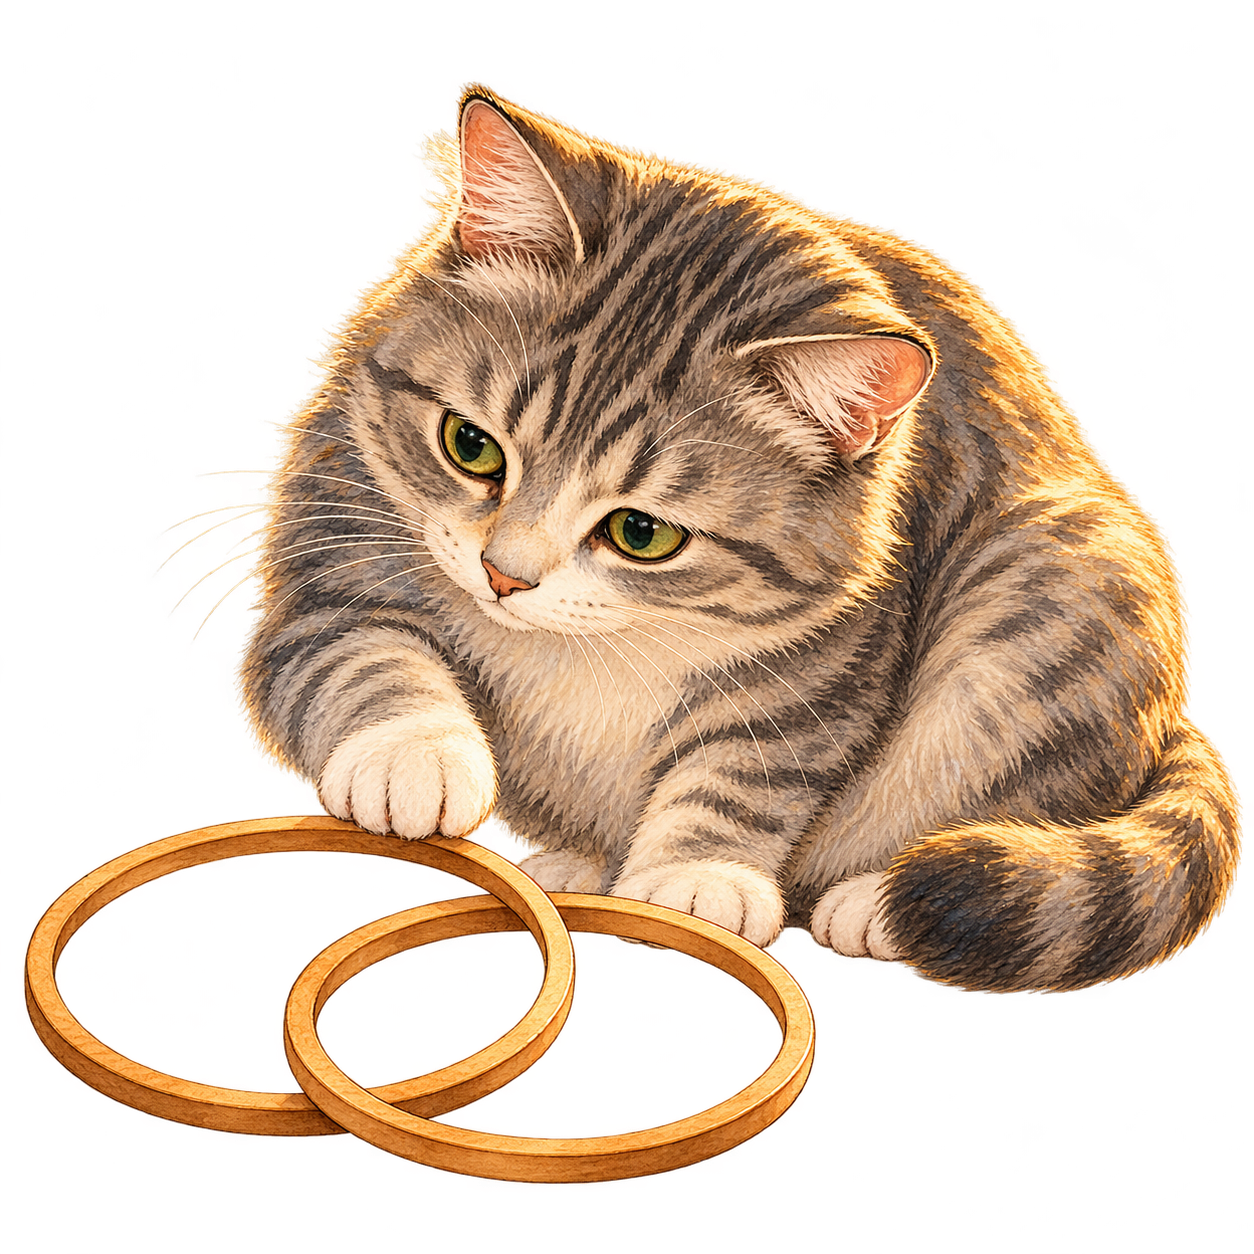
\includegraphics[width=54mm,height=58mm,keepaspectratio]{images/unique/art-32.png}
\end{wrapfigure}
\textbf{16.6.} Верна ли импликация: если число делится на \(4\), то оно чётное? Верно ли обратное?\par

\textbf{16.7.} Для делимости на \(6\) чётность — необходимое или достаточное условие?\par

\textbf{16.8.} Докажи, что сумма двух чётных целых чисел чётна.\par

\textbf{16.9.} Докажи, что квадрат нечётного целого числа нечётный.\par

\textbf{16.10.} Опровергни: если \(a^{2} = b^{2}\), то \(a = b\) для любых действительных \(a,\allowbreak b\).\par

\textbf{16.11.} Докажи по индукции: \(1 + 2 + \ldots  + n = \dfrac{n (n + 1)}{2}\) для натуральных \(n \ge  1\).\par

\textbf{16.12.} Докажи: если целое \(n\) нечётно, то \(n^{2}\) нечётно. Сформулируй равносильное утверждение через противоположное условие.\par
\par\WFclear\end{minipage}\end{lrbox}%
\ifdim\dimexpr\ht\CatFlowBox+\dp\CatFlowBox\relax<64mm\dp\CatFlowBox=\dimexpr64mm-\ht\CatFlowBox\relax\fi%
\noindent\usebox{\CatFlowBox}\par\addvspace{5pt}

\noindent\begin{minipage}[t]{\linewidth}\textbf{16.13.} Из жизни. В кафе все комплексные обеды включают напиток. Покупатель получил напиток. Обязательно ли он заказал комплексный обед?\par\end{minipage}\par
\noindent\begin{minipage}[t]{\linewidth}\textbf{16.14.} Из жизни. В группе \(20\) человек. Чай любят \(12\), кофе любят \(9\), оба напитка любят \(5\). Сколько любят хотя бы один из напитков и сколько не любят ни один?\par\end{minipage}\par
\noindent\begin{minipage}[t]{\linewidth}\textbf{16.15.} Из жизни. Объявление гласит: «Все автобусы на этом маршруте низкопольные». Какое наблюдение опровергнет утверждение? Сформулируй его отрицание.\par\end{minipage}\par
\noindent\begin{minipage}[t]{\linewidth}\textbf{16.16.}\starmark{} Из \(30\) учеников \(18\) изучают английский, \(16\) немецкий, каждый изучает хотя бы один из этих языков. Сколько изучают оба и сколько только английский?\begin{center}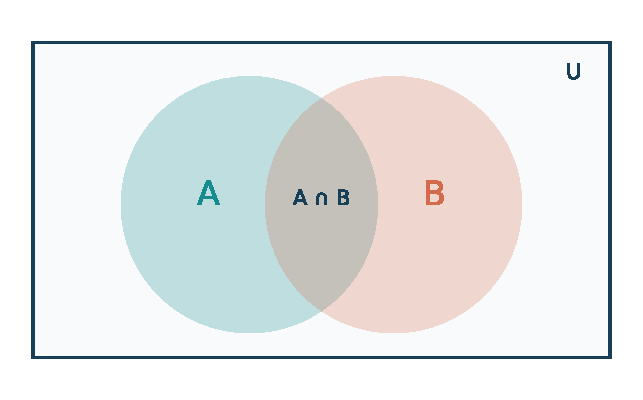
\includegraphics[width=.7\linewidth,height=45mm,keepaspectratio]{images/diagram-venn.pdf}\end{center}\par\end{minipage}\par
\noindent\begin{minipage}[t]{\linewidth}\textbf{16.17.}\starmark{} Докажи: если квадрат целого числа делится на \(3\), то само число делится на \(3\).\par\end{minipage}\par
\noindent\begin{minipage}[t]{\linewidth}\textbf{16.18.}\starmark{} Докажи по индукции: \(1 + 3 + 5 + \ldots  + (2 n - 1) = n^{2}\) для \(n \ge  1\).\par\end{minipage}\par
\noindent\begin{minipage}[t]{\linewidth}\textbf{16.19.}\starmark{} Для \(A,B\subseteq U\) докажи равенство \(A\setminus B=A\cap(U\setminus B)\) через принадлежность произвольного элемента.\par\end{minipage}\par
\noindent\begin{minipage}[t]{\linewidth}\textbf{16.20.}\starmark{} Докажи распределительный закон \(A\cap(B\cup C)=(A\cap B)\cup(A\cap C)\) через принадлежность элемента. Объясни, что нужно закрасить на диаграмме Венна для каждой стороны.\par\end{minipage}\par
\noindent\begin{minipage}[t]{\linewidth}\textbf{16.21.} Пусть \(A=\{1,2\}\), \(B=\{1,2,3\}\), \(C=\{2,4\}\). Определи истинность записей \(A\subseteq B\), \(A\subsetneq B\), \(C\subseteq B\), \(\varnothing\subseteq A\).\par\end{minipage}\par
\noindent\begin{minipage}[t]{\linewidth}\textbf{16.22.} Выпиши все элементы \(\mathcal P(\{a,b\})\), где \(a\ne b\). Сколько подмножеств имеет множество из четырёх элементов?\par\end{minipage}\par
\noindent\begin{minipage}[t]{\linewidth}\textbf{16.23.} Даны \(U=\{1,2,3,4,5,6,7,8\}\), \(A=\{2,4,6,8\}\), \(B=\{1,2,3,4\}\). Найди \(A\setminus B\), \(B\setminus A\), \(A\triangle B\), \(U\setminus A\), \(U\setminus B\).\par\end{minipage}\par
\noindent\begin{minipage}[t]{\linewidth}\textbf{16.24.} При \(A=\{1,2\}\), \(B=\{3\}\) выпиши \(A\times B\) и \(B\times A\). Равны ли эти множества? Сколько элементов в каждом?\par\end{minipage}\par
\noindent\begin{minipage}[t]{\linewidth}\textbf{16.25.} В группе пять человек: Аня, Боря, Вера, Глеб и Даша. Английским занимаются Аня, Вера и Даша, музыкой — Боря и Вера. Кто посещает ровно одно из двух занятий? Кто не посещает ни одно? Запиши ответы как симметрическую разность и дополнение объединения.\par\end{minipage}\par
\noindent\begin{minipage}[t]{\linewidth}\textbf{16.26.}\starmark{} Команду выбирают из шести человек: Ани, Бори, Веры, Глеба, Даши и Егора. Аня и Боря обязательно входят в команду, Вера не входит, а остальных можно включать или не включать. Сколько разных команд возможно? Объясни связь с множеством всех подмножеств.\par\end{minipage}\par
\endgroup

\backmatter\chapter*{Ответы и краткие решения}\addcontentsline{toc}{chapter}{Ответы и краткие решения}
\section*{Глава 1. Числа и свойства арифметических действий}
\begin{enumerate}[label={},leftmargin=3.2em,itemsep=6pt]
\item[\textbf{1.1.}] \(- 8 < - 3;\allowbreak 0 > - 5;\allowbreak - 4 < 4\).
\item[\textbf{1.2.}] \(- 12\).
\item[\textbf{1.3.}] \(3\).
\item[\textbf{1.4.}] \(- 3\).
\item[\textbf{1.5.}] \(- 8\).
\item[\textbf{1.6.}] \(7\). Делить на ноль нельзя.
\item[\textbf{1.7.}] \(- 14\).
\item[\textbf{1.8.}] \(- 20\).
\item[\textbf{1.9.}] \(- 26\).
\item[\textbf{1.10.}] \(- 4\). В записи \(- 2^{2}\) степень относится только к двойке.
\item[\textbf{1.11.}] \(- 2 {}^{\circ} C\).
\item[\textbf{1.12.}] На уровне \(2\).
\item[\textbf{1.13.}] \(115\) очков.
\item[\textbf{1.14.}\starmark] \(3\). Скобки равны \(8\) и \(3\), поэтому \(- 6 + 9 = 3\).
\item[\textbf{1.15.}\starmark] \((18 - 6) : (3 + 1) = 3\).
\item[\textbf{1.16.}\starmark] \(8\) верных и \(4\) неверных: \(8 \cdot  5 - 4 \cdot  3 = 28\).
\item[\textbf{1.17.}] База \(n=0\): \(0=0\). Переход: если сумма до \(n\) равна \(\frac{n(n+1)}2\), то сумма до \(n+1\) равна \(\frac{n(n+1)}2+(n+1)=\frac{(n+1)(n+2)}2\).
\item[\textbf{1.18.}] База \(n=1\): \(1=1^2\). При переходе добавляется следующее нечётное число \(2n+1\), а \(n^2+(2n+1)=(n+1)^2\).
\item[\textbf{1.19.}\starmark] База \(n=0\): обе части нулевые. Переход: \(\frac{n(n+1)(2n+1)}6+(n+1)^2=\frac{(n+1)(n+2)(2n+3)}6\). Это нужная формула с \(n+1\) вместо \(n\).
\item[\textbf{1.20.}] База \(n=0\): \(1=2-1\). Переход: к сумме до \(n\) добавляется \(2^{n+1}\), поэтому новая сумма равна \((2^{n+1}-1)+2^{n+1}=2^{n+2}-1\).
\item[\textbf{1.21.}] База \(n=0\): \(1\ge1\). Если \(3^n\ge2n+1\), то \(3^{n+1}\ge3(2n+1)=6n+3\ge2n+3=2(n+1)+1\), поскольку \(n\ge0\).
\item[\textbf{1.22.}] База \(n=4\): \(16=16\). Если \(2^n\ge n^2\), то \(2^{n+1}\ge2n^2\ge(n+1)^2\). Последнее неравенство верно при \(n\ge4\), так как \(2n^2-(n+1)^2=(n-1)^2-2\ge7>0\).
\item[\textbf{1.23.}\starmark] База \(n=0\): обе части нулевые. Переход: \(\frac{n^2(n+1)^2}{4}+(n+1)^3=\frac{(n+1)^2(n+2)^2}{4}=\left(\frac{(n+1)(n+2)}2\right)^2\).
\item[\textbf{1.24.}\starmark] База \(n=1\): равенство. По предположению \((1+x)^n\ge1+nx\). Умножая на \(1+x\ge0\), сохраняем направление неравенства: \((1+x)^{n+1}\ge(1+nx)(1+x)=1+(n+1)x+nx^2\ge1+(n+1)x\). Без неотрицательности множителя направление могло бы измениться.
\item[\textbf{1.25.}] Из коммутативности \(x+a=0\). Тогда \(x=x+0=x+(a+y)=(x+a)+y=0+y=y\).
\item[\textbf{1.26.}] Если один множитель нулевой, произведение равно нулю. Обратно: пусть \(ab=0\). При \(a=0\) утверждение уже выполнено. При \(a\ne0\) умножим равенство на \(\frac1a\) и воспользуемся ассоциативностью: \(b=\frac1a(ab)=\frac1a\cdot0=0\).
\end{enumerate}
\section*{Глава 2. Делимость, простые числа, НОД и НОК}
\begin{enumerate}[label={},leftmargin=3.2em,itemsep=6pt]
\item[\textbf{2.1.}] \(1,\allowbreak 2,\allowbreak 3,\allowbreak 4,\allowbreak 6,\allowbreak 9,\allowbreak 12,\allowbreak 18,\allowbreak 36\).
\item[\textbf{2.2.}] \(1,\allowbreak 2,\allowbreak 3,\allowbreak 4,\allowbreak 6,\allowbreak 8,\allowbreak 12,\allowbreak 16,\allowbreak 24,\allowbreak 48\).
\item[\textbf{2.3.}] \(1,\allowbreak 2,\allowbreak 5,\allowbreak 10\).
\item[\textbf{2.4.}] \(21,\allowbreak 28,\allowbreak 35,\allowbreak 42,\allowbreak 49,\allowbreak 56\).
\item[\textbf{2.5.}] \(104\).
\item[\textbf{2.6.}] Простые: \(17,\allowbreak 31,\allowbreak 53\). Составные: \(25,\allowbreak 39,\allowbreak 49,\allowbreak 51\).
\item[\textbf{2.7.}] \(23,\allowbreak 29,\allowbreak 31,\allowbreak 37\).
\item[\textbf{2.8.}] Нет: такое натуральное число не меньше \(10\) и имеет делитель \(2\), отличный от \(1\) и самого числа.
\item[\textbf{2.9.}] Нет, например \(9 = 3 \cdot  3\).
\item[\textbf{2.10.}] На \(3\) и на \(9\) делятся \(126,\allowbreak 234,\allowbreak 405,\allowbreak 702;\allowbreak 517\) не делится ни на \(3\), ни на \(9\).
\item[\textbf{2.11.}] \(230,\allowbreak 480\).
\item[\textbf{2.12.}] \(2,\allowbreak 5,\allowbreak 8\).
\item[\textbf{2.13.}] \(0\) или \(9\).
\item[\textbf{2.14.}] \(0,\allowbreak 6\).
\item[\textbf{2.15.}] \(2^{3} \cdot  3^{2}\).
\item[\textbf{2.16.}] \(2 \cdot  3 \cdot  5^{2}\).
\item[\textbf{2.17.}] \(2^{2} \cdot  3^{2} \cdot  7\).
\item[\textbf{2.18.}] \(90 = 2 \cdot  3^{2} \cdot  5\).
\item[\textbf{2.19.}] НОД \(= 12\); НОК \(= 72\).
\item[\textbf{2.20.}] НОД \(= 9\); НОК \(= 90\).
\item[\textbf{2.21.}] НОД \(= 1\); НОК \(= 120\).
\item[\textbf{2.22.}] НОД \(= 6\); НОК \(= 180\).
\item[\textbf{2.23.}] \(12\) наборов, в каждом \(2\) карандаша и \(3\) ручки.
\item[\textbf{2.24.}] В 9:36.
\item[\textbf{2.25.}] Сторона \(12\) см; \(35\) квадратов.
\item[\textbf{2.26.}] \(1,\allowbreak 2,\allowbreak 3,\allowbreak 4,\allowbreak 6,\allowbreak 8,\allowbreak 12,\allowbreak 24\).
\item[\textbf{2.27.}] \(6,\allowbreak 12,\allowbreak 18,\allowbreak 24,\allowbreak 30\).
\item[\textbf{2.28.}] \(2,\allowbreak 13,\allowbreak 29\). Число \(1\) не простое и не составное.
\item[\textbf{2.29.}] На все перечисленные.
\item[\textbf{2.30.}] \(2^{2} \cdot  3 \cdot  7\).
\item[\textbf{2.31.}] НОД \(= 6\); НОК \(= 36\).
\item[\textbf{2.32.}] \(14\) подарков; по \(3\) яблока и \(4\) мандарина.
\item[\textbf{2.33.}] Через \(24\) секунды.
\item[\textbf{2.34.}] Нет: \(97\) — простое число.
\item[\textbf{2.35.}\starmark] \(73\): НОК\((6,8,\allowbreak 9) = 72\), затем прибавляем \(1\).
\item[\textbf{2.36.}\starmark] \(36\). Решение: \(\frac{6 \cdot 180}{30} = 36\).
\item[\textbf{2.37.}\starmark] \(3150\) и \(3555\). Сумма цифр равна соответственно \(9\) и \(18\).
\item[\textbf{2.38.}] Если \(d\mid a\) и \(d\mid b\), то \(a=du\), \(b=dv\), поэтому \(a-b=d(u-v)\) и \(d\mid(a-b)\). Обратно, если \(d\mid b\) и \(d\mid(a-b)\), то \(d\mid((a-b)+b)=a\). Множества общих делителей совпадают, значит, совпадают и их наибольшие элементы.
\item[\textbf{2.39.}] Если \(a=1\) или \(b=1\), вывод немедленно следует из условия. Иначе разложим оба множителя на простые. Их произведение даёт разложение \(ab\). Поскольку \(p\mid ab\), число \(p\) входит в разложение произведения; по единственности разложения оно входит в разложение хотя бы одного множителя. Значит, \(p\) делит этот множитель.
\end{enumerate}
\section*{Глава 3. Обыкновенные дроби}
\begin{enumerate}[label={},leftmargin=3.2em,itemsep=6pt]
\item[\textbf{3.1.}] \(\frac{3}{4}\).
\item[\textbf{3.2.}] \(3 \frac{2}{5}\).
\item[\textbf{3.3.}] \(\frac{17}{7}\).
\item[\textbf{3.4.}] \(\frac{5}{8} > \frac{7}{12}\).
\item[\textbf{3.5.}] \(- \frac{1}{12}\).
\item[\textbf{3.6.}] \(\frac{31}{45}\).
\item[\textbf{3.7.}] \(- \frac{2}{3}\).
\item[\textbf{3.8.}] \(\frac{3}{2}\).
\item[\textbf{3.9.}] \(\frac{1}{2}\).
\item[\textbf{3.10.}] \(1\).
\item[\textbf{3.11.}] \(\frac{2}{3}\).
\item[\textbf{3.12.}] \(32\) страницы.
\item[\textbf{3.13.}] \(\frac{17}{12}\) кг, или \(1 \frac{5}{12}\) кг.
\item[\textbf{3.14.}] \(6\) стаканов.
\item[\textbf{3.15.}] \(9\) км.
\item[\textbf{3.16.}\starmark] \(-\frac{1}{4}\). Решение: \((-\frac{1}{12}) : (\frac{1}{9}) + \frac{1}{2} = -\frac{3}{4} + \frac{1}{2} = -\frac{1}{4}\).
\item[\textbf{3.17.}\starmark] \(180\) страниц: осталось \((\frac{2}{3}) \cdot  (\frac{3}{5}) = \frac{2}{5}\) книги.
\item[\textbf{3.18.}\starmark] \(30\) л: осталось \((\frac{3}{4}) \cdot  (\frac{2}{3}) = \frac{1}{2}\) бака.
\item[\textbf{3.19.}] Умножение равенства дробей на ненулевое число \(bd\) даёт \(ad=bc\). Обратно, деление \(ad=bc\) на \(bd\ne0\) даёт равенство дробей.
\item[\textbf{3.20.}] Для каждого \(k\ge1\) имеем \(\frac1{k(k+1)}=\frac1k-\frac1{k+1}\). При сложении соседние дроби взаимно уничтожаются: \(\left(1-\frac12\right)+\left(\frac12-\frac13\right)+\cdots+\left(\frac1n-\frac1{n+1}\right)=1-\frac1{n+1}=\frac n{n+1}\).
\end{enumerate}
\section*{Глава 4. Десятичные дроби и проценты}
\begin{enumerate}[label={},leftmargin=3.2em,itemsep=6pt]
\item[\textbf{4.1.}] \(3,836\).
\item[\textbf{4.2.}] \(5,53\).
\item[\textbf{4.3.}] \(0,12\).
\item[\textbf{4.4.}] \(60\).
\item[\textbf{4.5.}] \(0,875\).
\item[\textbf{4.6.}] \(\frac{1}{8}\).
\item[\textbf{4.7.}] \(0{,}(6)\).
\item[\textbf{4.8.}] \(3,14;\allowbreak 3,142\).
\item[\textbf{4.9.}] \(36\).
\item[\textbf{4.10.}] \(180\).
\item[\textbf{4.11.}] На \(15 \%\).
\item[\textbf{4.12.}] \(960\) рублей; снижение на \(4 \%\).
\item[\textbf{4.13.}] \(225\) рублей.
\item[\textbf{4.14.}] \(4080\) рублей.
\item[\textbf{4.15.}] \(13,33\) км; после округления \(13,3\) км.
\item[\textbf{4.16.}\starmark] \(3000\) рублей: \(\frac{2160}{0,8 \cdot  0,9}\).
\item[\textbf{4.17.}\starmark] На \(20 \%\). Решение: \(\frac{25}{125} = 0{,}2 = 20 \%\).
\item[\textbf{4.18.}\starmark] \(16 \%\). Решение: \(\frac{20 + 60}{500} \cdot 100 \% = 16 \%\).
\item[\textbf{4.19.}] Если исходная цена \(S>0\), конечная цена равна \(S\left(1+\frac p{100}\right)\left(1+\frac q{100}\right)=S\left(1+\frac{p+q}{100}+\frac{pq}{10000}\right)\). Прибавка, делённая на \(S\) и умноженная на \(100\), равна \(p+q+\frac{pq}{100}\).
\item[\textbf{4.20.}\starmark] Если \(\frac pq=\frac m{10^k}\), то \(p10^k=mq\). Поскольку \(p\) и \(q\) взаимно просты, все простые множители \(q\), с их кратностями, должны входить в \(10^k=2^k5^k\). Поэтому \(q=2^{\alpha}5^{\beta}\). Обратно, при таком знаменателе возьмём \(k=\max(\alpha,\beta)\) и домножим числитель и знаменатель на \(2^{k-\alpha}5^{k-\beta}\). Знаменатель станет \(10^k\), а значит, дробь имеет конечную десятичную запись.
\end{enumerate}
\section*{Глава 5. Отношения и пропорции}
\begin{enumerate}[label={},leftmargin=3.2em,itemsep=6pt]
\item[\textbf{5.1.}] \(3 : 4\).
\item[\textbf{5.2.}] \(x = 12\).
\item[\textbf{5.3.}] \(x = 6\).
\item[\textbf{5.4.}] \(24\) и \(40\).
\item[\textbf{5.5.}] \(750\) г.
\item[\textbf{5.6.}] \(288\) рублей.
\item[\textbf{5.7.}] \(3,5\) км.
\item[\textbf{5.8.}] За \(4\) дня.
\item[\textbf{5.9.}] \(2\) часа.
\item[\textbf{5.10.}] \(0,6\) л сока; \(0,9\) л воды.
\item[\textbf{5.11.}] \(y = 12\); удвоится.
\item[\textbf{5.12.}] \(y = 4\); уменьшится вдвое.
\item[\textbf{5.13.}] \(750\) г.
\item[\textbf{5.14.}] За \(6\) часов.
\item[\textbf{5.15.}] \(0,25\) л сиропа и \(1,75\) л воды.
\item[\textbf{5.16.}\starmark] \(10\) дней: \(6 \cdot  8 \cdot  \frac{5}{4 \cdot  6}\).
\item[\textbf{5.17.}\starmark] \(7\) л: \(\frac{2 k}{5 k + 3} = \frac{1}{4}\) даёт \(k = 1\).
\item[\textbf{5.18.}\starmark] При равных временах \(75\) км/ч. При равных расстояниях \(72\) км/ч: \(\frac{2}{\frac{1}{60} + \frac{1}{90}}\).
\item[\textbf{5.19.}] Из условия \(a=kb\), \(c=kd\). Тогда \(\frac{a+c}{b+d}=\frac{k(b+d)}{b+d}=k\); деление допустимо, поскольку \(b+d>0\).
\item[\textbf{5.20.}\starmark] Из исходного неравенства следует \(bc-ad>0\). Разности равны \(\frac{a+c}{b+d}-\frac ab=\frac{bc-ad}{b(b+d)}>0\) и \(\frac cd-\frac{a+c}{b+d}=\frac{bc-ad}{d(b+d)}>0\). Обе границы доказаны.
\end{enumerate}
\section*{Глава 6. Степени с целым показателем}
\begin{enumerate}[label={},leftmargin=3.2em,itemsep=6pt]
\item[\textbf{6.1.}] \(32\).
\item[\textbf{6.2.}] \(81\) и \(- 81\).
\item[\textbf{6.3.}] \(\frac{9}{8}\).
\item[\textbf{6.4.}] \(5^{7}\).
\item[\textbf{6.5.}] \(2^{5}\).
\item[\textbf{6.6.}] \(3^{8}\).
\item[\textbf{6.7.}] \(\frac{9}{4}\).
\item[\textbf{6.8.}] \(100\).
\item[\textbf{6.9.}] \(5,6 \cdot  10^{- 4}\).
\item[\textbf{6.10.}] \(720000\).
\item[\textbf{6.11.}] \(a^{3}\).
\item[\textbf{6.12.}] \(- 1\).
\item[\textbf{6.13.}] \(2^{8} = 256\) бактерий.
\item[\textbf{6.14.}] \(10^{6}\) м\(^{2}\) \(= 1000000\) м\(^{2}\).
\item[\textbf{6.15.}] \(1,2 \cdot  10^{9}\) байт.
\item[\textbf{6.16.}\starmark] \(16 = 2^{4}\).
\item[\textbf{6.17.}\starmark] \(\frac{9}{2}\). Решение: \(\frac{3^{4} \cdot 2}{3^{2} \cdot 4} = \frac{9}{2}\).
\item[\textbf{6.18.}\starmark] Сначала \(2\) МБ; через \(6\) дней \(1458\) МБ.
\item[\textbf{6.19.}] \(a^m\) содержит \(m\) множителей \(a\), а \(a^n\) — ещё \(n\). По сочетательному свойству их произведение состоит из \(m+n\) таких множителей, то есть равно \(a^{m+n}\).
\item[\textbf{6.20.}] \(a^{-m}a^{-n}=\frac1{a^m}\frac1{a^n}=\frac1{a^{m+n}}=a^{-(m+n)}\). Все знаменатели ненулевые, поскольку \(a\neq0\).
\end{enumerate}
\section*{Глава 7. Корни и действительные числа}
\begin{enumerate}[label={},leftmargin=3.2em,itemsep=6pt]
\item[\textbf{7.1.}] \(9;\allowbreak - 3\).
\item[\textbf{7.2.}] \(\frac{7}{10}\).
\item[\textbf{7.3.}] \(6 \sqrt{2}\).
\item[\textbf{7.4.}] \(5 \sqrt{2}\).
\item[\textbf{7.5.}] \(\sqrt{45}\).
\item[\textbf{7.6.}] \(6\).
\item[\textbf{7.7.}] \(5\).
\item[\textbf{7.8.}] \(7\).
\item[\textbf{7.9.}] Между \(5\) и \(6\).
\item[\textbf{7.10.}] \(\sqrt{7} < 2,7\), так как \(7 < 2,7^{2} = 7,29\).
\item[\textbf{7.11.}] \(\sqrt{16},\allowbreak - \frac{3}{7},\allowbreak 0{,}(3)\).
\item[\textbf{7.12.}] \(\sqrt{- 9}\) не существует; \(\sqrt[3]{- 8} = - 2\).
\item[\textbf{7.13.}] \(7\) м.
\item[\textbf{7.14.}] \(5\) м.
\item[\textbf{7.15.}] \(0,5\) м, или \(50\) см.
\item[\textbf{7.16.}\starmark] \(2\sqrt{3}\). Решение: \(4\sqrt{3} + 5\sqrt{3} - 7\sqrt{3} = 2\sqrt{3}\).
\item[\textbf{7.17.}\starmark] Квадрат левой части \(5 + 2 \sqrt{6} < 10\), поскольку \(\sqrt{6} < \frac{5}{2}\). Поэтому исходное утверждение неверно: \(\sqrt{2} + \sqrt{3} < \sqrt{10}\).
\item[\textbf{7.18.}\starmark] \(4\) м и \(12\) м; диагональ \(4 \sqrt{10}\) м.
\item[\textbf{7.19.}] \(|x|\geq0\) и \(|x|^n=x^n\). По определению арифметического корня единственное неотрицательное число с такой \(n\)-й степенью равно \(|x|\).
\item[\textbf{7.20.}] Если \(u=\sqrt[n]a\), то \((-u)^n=-u^n=-a\), так как \(n\) нечётно. По единственности нечётного корня \(\sqrt[n]{-a}=-u\).
\item[\textbf{7.21.}] \(3\), \(-2\), \(2\) соответственно.
\item[\textbf{7.22.}] \(\sqrt[4]{-16}\) не определено в \(\mathbb R\); \(\sqrt[3]{-64}=-4\); \(\sqrt[6]0=0\).
\item[\textbf{7.23.}] \(\sqrt[6]{x^6}=|x|\), \(\sqrt[5]{x^5}=x\).
\item[\textbf{7.24.}] \(\sqrt[4]{48}=2\sqrt[4]3\); \(\frac{\sqrt[3]{54}}{\sqrt[3]2}=\sqrt[3]{27}=3\).
\item[\textbf{7.25.}] \(4\), \(-\frac12\), \(\frac18\) соответственно. В первых двух выражениях знаменатели несократимых показателей нечётны.
\item[\textbf{7.26.}] Первое уравнение: \(x+7=16\), поэтому \(x=9\). Второе: \(2x-1=-27\), поэтому \(x=-13\). Подстановка подтверждает оба ответа.
\item[\textbf{7.27.}\starmark] Для четвёртого корня требуется \(x-2\geq0\), а знаменатель исключает \(x=2\). Кубический корень ограничений не добавляет. Область определения: \((2;+\infty)\).
\item[\textbf{7.28.}\starmark] Получаем \(|x-1|=2-x\), поэтому \(x\leq2\). При \(x<1\) равенство \(1-x=2-x\) невозможно; при \(1\leq x\leq2\) получаем \(x-1=2-x\), откуда \(x=\frac32\).
\end{enumerate}
\section*{Глава 8. Модуль и числовые промежутки}
\begin{enumerate}[label={},leftmargin=3.2em,itemsep=6pt]
\item[\textbf{8.1.}] \(11\).
\item[\textbf{8.2.}] \(3\).
\item[\textbf{8.3.}] \(11\).
\item[\textbf{8.4.}] \(| - 6 | > | 5 |\).
\item[\textbf{8.5.}] \((- 2;\allowbreak 3]\).
\item[\textbf{8.6.}] \(- 4 \le  x < 1\).
\item[\textbf{8.7.}] \(- 2,\allowbreak - 1,\allowbreak 0,\allowbreak 1,\allowbreak 2\).
\item[\textbf{8.8.}] \((1;\allowbreak 4]\).
\item[\textbf{8.9.}] \((- \infty ;\allowbreak 5)\).
\item[\textbf{8.10.}] \(x = - 5\) или \(x = 5\).
\item[\textbf{8.11.}] \(- 1 < x < 5\).
\item[\textbf{8.12.}] \(| x |;\allowbreak 4\).
\item[\textbf{8.13.}] На \(40 {}^{\circ} C\).
\item[\textbf{8.14.}] \(| x - 50 | \le  0,2;\allowbreak [49,8;\allowbreak 50,2]\) мм.
\item[\textbf{8.15.}] \(120 \le  h < 190;\allowbreak [120;\allowbreak 190)\); при \(190\) см нельзя.
\item[\textbf{8.16.}\starmark] \(x = - 2\) или \(x = 4\). Между \(- 1\) и \(3\) сумма равна \(4\).
\item[\textbf{8.17.}\starmark] \(- 2,\allowbreak - 1,\allowbreak 2,\allowbreak 3\): допустимый отрезок \([- 2;\allowbreak 3]\), исключаются \(0\) и \(1\).
\item[\textbf{8.18.}\starmark] \((20;\allowbreak 23]\): пересечение \([17;\allowbreak 23]\) и \((20;\allowbreak 28)\).
\item[\textbf{8.19.}] Из \(|a|=|(a-b)+b|\leq|a-b|+|b|\) следует \(|a|-|b|\leq|a-b|\). После перестановки \(a,b\) получаем \(|b|-|a|\leq|a-b|\). Вместе эти два неравенства дают требуемое.
\item[\textbf{8.20.}] Для любого \(u\) и \(r\geq0\) условие \(|u|\leq r\) равносильно \(-r\leq u\leq r\), что проверяется по случаям \(u\geq0\) и \(u<0\). Подставляем \(u=x-a\) и прибавляем \(a\) к обеим границам.
\end{enumerate}
\section*{Глава 9. Преобразование алгебраических выражений}
\begin{enumerate}[label={},leftmargin=3.2em,itemsep=6pt]
\item[\textbf{9.1.}] \(4 x - 17\).
\item[\textbf{9.2.}] \(6 a + 2 b\).
\item[\textbf{9.3.}] \(x^{2} + 6 x + 9\).
\item[\textbf{9.4.}] \(4 x^{2} - 1\).
\item[\textbf{9.5.}] \(3 x (2 x - 3)\).
\item[\textbf{9.6.}] \((x - 4) (x + 4)\).
\item[\textbf{9.7.}] \((x + 2) (x + 3)\).
\item[\textbf{9.8.}] \(x + 1\) при \(x \ne  1\).
\item[\textbf{9.9.}] \(\frac{7}{2 x},\allowbreak x \ne  0\).
\item[\textbf{9.10.}] \(\frac{a}{b},\allowbreak a \ne  0\) и \(b \ne  0\).
\item[\textbf{9.11.}] \(\frac{x - 2}{x + 2},\allowbreak x \ne  - 2\).
\item[\textbf{9.12.}] \(\sqrt{5} + 2\).
\item[\textbf{9.13.}] \(3 x + 2 (x - 100) = 5 x - 200\) рублей.
\item[\textbf{9.14.}] \(x^{2} + 7 x + 10\) м\(^{2}\).
\item[\textbf{9.15.}] \((x + 3)^{2} - x^{2} = 6 x + 9\) м\(^{2}\).
\item[\textbf{9.16.}\starmark] \(\frac{x + 3}{x + 2},\allowbreak x \ne  3\) и \(x \ne  - 2\).
\item[\textbf{9.17.}\starmark] \(1\) при \(x \ne  - 1\) и \(x \ne  1\).
\item[\textbf{9.18.}\starmark] Разность равна \(4 ab\); при данных значениях \(39964\).
\item[\textbf{9.19.}] После раскрытия квадратов левая часть равна \(a^2+2ab+b^2+a^2-2ab+b^2=2a^2+2b^2\).
\item[\textbf{9.20.}] Общий знаменатель равен \((x-1)(x+1)=x^2-1\), а числитель разности — \((x+1)-(x-1)=2\). При \(x=1\) или \(x=-1\) один из исходных знаменателей нулевой, поэтому эти значения исключаются.
\end{enumerate}
\section*{Глава 10. Комбинаторика и бином Ньютона}
\begin{enumerate}[label={},leftmargin=3.2em,itemsep=6pt]
\item[\textbf{10.1.}] \(5+3=8\) способов: группы книг не пересекаются, поэтому применяется правило суммы.
\item[\textbf{10.2.}] \(4\cdot3\cdot2=24\) комплекта по правилу произведения.
\item[\textbf{10.3.}] а) Порядок важен, повторений нет: размещение без повторений. б) Порядок не важен, повторений нет: сочетание без повторений. в) Порядок важен, повторения разрешены: размещение с повторениями. г) Порядок не важен, повторения разрешены: сочетание с повторениями.
\item[\textbf{10.4.}] \(120\), \(1\), \(42\); в последнем выражении сокращаются множители от \(1\) до \(5\), остаётся \(7\cdot6\).
\item[\textbf{10.5.}] \(6!=720\) способов.
\item[\textbf{10.6.}] \(\frac{5!}{2!2!}=30\): буквы Т и О встречаются по два раза.
\item[\textbf{10.7.}] \(A_8^3=8\cdot7\cdot6=336\) вариантов.
\item[\textbf{10.8.}] \(\binom83=\frac{8!}{3!5!}=56\) выборов.
\item[\textbf{10.9.}] \(10^4=10000\) кодов: для каждой позиции независимо есть \(10\) вариантов.
\item[\textbf{10.10.}] \(9\cdot9\cdot8\cdot7=4536\). Для первой цифры есть \(9\) ненулевых вариантов; для второй снова \(9\) вариантов, включая ноль и исключая уже выбранную цифру.
\item[\textbf{10.11.}] \(\overline C_4^3=\binom{4+3-1}{3}=\binom63=20\) выборов.
\item[\textbf{10.12.}] Нужно посчитать тройки \((x_1,x_2,x_3)\) неотрицательных целых чисел с суммой \(7\). По методу звёздочек и перегородок ответ \(\binom{7+3-1}{3-1}=\binom92=36\).
\item[\textbf{10.13.}] \(\binom n2=\frac{n(n-1)}2=45\), значит, \(n(n-1)=90\). Подходит \(n=10\). Другого решения при \(n\ge2\) нет: произведение \(n(n-1)\) строго возрастает с ростом \(n\).
\item[\textbf{10.14.}] \(\binom83=\binom72+\binom73=21+35=56\).
\item[\textbf{10.15.}] \(x^4+8x^3+24x^2+32x+16\).
\item[\textbf{10.16.}] \(\binom73\,2^4=35\cdot16=560\).
\item[\textbf{10.17.}] При \(n=0\) обе части равны \(1\). При \(n\ge1\) подставим \(a=b=1\) в бином Ньютона: получим сумму всех коэффициентов и \(2^n\). Есть и подсчёт двумя способами: каждое из \(n\) различных элементов можно включить или не включить в подмножество, всего \(2^n\) вариантов; группировка по числу выбранных элементов даёт левую часть.
\item[\textbf{10.18.}\starmark] В группе может быть \(2\), \(3\) или \(4\) девушки. Эти случаи не пересекаются. Ответ: \(\binom42\binom63+\binom43\binom62+\binom44\binom61=120+60+6=186\).
\item[\textbf{10.19.}\starmark] Из \(10^5\) кодов вычтем \(9^5\) кодов без нуля и \(9^5\) кодов без единицы. Коды, в которых нет ни нуля, ни единицы, были вычтены дважды; их \(8^5\), поэтому их нужно прибавить один раз. Ответ: \(10^5-2\cdot9^5+8^5=14670\).
\item[\textbf{10.20.}\starmark] Разделим \(m+n\) различных элементов на две непересекающиеся группы размеров \(m\) и \(n\). Всего выбрать \(r\) элементов можно \(\binom{m+n}{r}\) способами. Если из первой группы взято ровно \(k\) элементов, из второй нужно взять \(r-k\); вариантов \(\binom mk\binom n{r-k}\). Суммирование по всем \(k\) даёт левую часть. Невозможные случаи дают ноль по условленному обозначению.
\end{enumerate}
\section*{Глава 11. Уравнения, системы и неравенства}
\begin{enumerate}[label={},leftmargin=3.2em,itemsep=6pt]
\item[\textbf{11.1.}] \(x = 6\).
\item[\textbf{11.2.}] \(x = - 5\).
\item[\textbf{11.3.}] \(x = 2\) или \(3\).
\item[\textbf{11.4.}] \(x = - 2\) или \(2\).
\item[\textbf{11.5.}] \(x = 5\); ОДЗ: \(x \ne  2\).
\item[\textbf{11.6.}] \(x = 4,\allowbreak y = 3\).
\item[\textbf{11.7.}] \(x < - 4\).
\item[\textbf{11.8.}] \([- 3;\allowbreak 3]\).
\item[\textbf{11.9.}] \((- \infty ;\allowbreak - 2) \cup  (1;\allowbreak + \infty )\).
\item[\textbf{11.10.}] \((- 1;\allowbreak 3]\).
\item[\textbf{11.11.}] \(x = - 2\) или \(3\).
\item[\textbf{11.12.}] \(x=2\). ОДЗ: \(x\ge-2\). Для выполнения равенства необходимо \(x\ge0\). После возведения в квадрат кандидаты \(2\) и \(-1\); проверка исключает \(-1\).
\item[\textbf{11.13.}] \(12\) км.
\item[\textbf{11.14.}] \(120\) рублей.
\item[\textbf{11.15.}] \(5\) билетов.
\item[\textbf{11.16.}\starmark] \(x = 3\). После возведения в квадрат корни \(3\) и \(- 1;\allowbreak - 1\) посторонний.
\item[\textbf{11.17.}\starmark] \(x < - 3\): дробь после переноса равна \(- \frac{5}{x + 3}\).
\item[\textbf{11.18.}\starmark] \(5\) м и \(12\) м: \(x (17 - x) = 60\).
\item[\textbf{11.19.}] По формуле корней \(x_{1,2}=\frac{-b\pm\sqrt{b^2-4ac}}{2a}\). Их сумма равна \(-\frac ba\), произведение — \(\frac{b^2-(b^2-4ac)}{4a^2}=\frac ca\). При нулевом дискриминанте обе записи обозначают один и тот же корень, взятый дважды.
\item[\textbf{11.20.}] Уравнение равносильно \((2ax+b)^2=D\), так как \(4a(ax^2+bx+c)=(2ax+b)^2-D\) и \(4a\neq0\). Квадрат действительного числа неотрицателен, поэтому \(D\geq0\) необходимо. При \(D\geq0\) числа \(x=\frac{-b\pm\sqrt D}{2a}\) удовлетворяют равенству, поэтому условие достаточно.
\item[\textbf{11.21.}] \(x^3-8=(x-2)(x^2+2x+4)\). Второй множитель равен \((x+1)^2+3>0\), поэтому единственный действительный корень \(x=2\).
\item[\textbf{11.22.}] \(x^3+27=(x+3)(x^2-3x+9)\). Второй множитель равен \((x-\frac32)^2+\frac{27}4>0\), поэтому \(x=-3\).
\item[\textbf{11.23.}] \(x^3-6x^2+11x-6=(x-1)(x-2)(x-3)\). Корни: \(1,2,3\).
\item[\textbf{11.24.}] Группировка даёт \(x^2(2x-3)-4(2x-3)=(2x-3)(x-2)(x+2)\). Корни: \(-2,\frac32,2\).
\item[\textbf{11.25.}\starmark] Получаем \(t^3-3t-2=(t-2)(t+1)^2=0\). Поэтому \(t=2\) или \(t=-1\), а \(x=4\) или \(x=1\). Корень \(x=1\) имеет кратность \(2\).
\item[\textbf{11.26.}] При \(u=x^2\geq0\) получаем \((u-1)(u-4)=0\). Поэтому \(x=-2,-1,1,2\).
\item[\textbf{11.27.}] \(u^2+3u-4=(u-1)(u+4)=0\). Значение \(u=-4\) невозможно для \(u=x^2\). При \(u=1\) получаем \(x=-1\) или \(x=1\).
\item[\textbf{11.28.}\starmark] \(x\neq0\). Получаем \(t^2-5t+4=0\), откуда \(t=1\) или \(t=4\). Значение \(1\) не подходит, а \(t=4\) даёт \(x^2-4x+1=0\). Ответ: \(x=2-\sqrt3\) или \(x=2+\sqrt3\).
\end{enumerate}
\section*{Глава 12. Последовательности и прогрессии}
\begin{enumerate}[label={},leftmargin=3.2em,itemsep=6pt]
\item[\textbf{12.1.}] \(1,4,7,10,13\); \(a_{10}=28\).
\item[\textbf{12.2.}] \(-1,\frac12,-\frac13,\frac14\). Член \(a_{25}\) отрицателен, \(a_{26}\) положителен.
\item[\textbf{12.3.}] \(2,3,5,9,17\).
\item[\textbf{12.4.}] \(d=4\), \(a_n=3+4(n-1)=4n-1\).
\item[\textbf{12.5.}] \(a_8=7+7(-3)=-14\).
\item[\textbf{12.6.}] \(d=\frac{35-11}{9-3}=4\), \(a_1=11-2\cdot4=3\).
\item[\textbf{12.7.}] \(a_{20}=43\), \(S_{20}=\frac{20(5+43)}2=480\).
\item[\textbf{12.8.}] \(q=-2\), \(a_n=3(-2)^{n-1}\), \(a_6=-96\).
\item[\textbf{12.9.}] \(a_5=81(\frac13)^4=1\).
\item[\textbf{12.10.}] \(q^3=\frac{48}{6}=8\), поэтому \(q=2\), \(a_1=3\).
\item[\textbf{12.11.}] \(128=2^7\), поэтому слагаемых \(8\). Сумма \(S_8=\frac{1-2^8}{1-2}=255\).
\item[\textbf{12.12.}] \(q=-\frac13\), \(|q|<1\), поэтому \(S=\frac{18}{1+\frac13}=\frac{27}{2}\).
\item[\textbf{12.13.}] В двенадцатую неделю \(650\) рублей; всего \(\frac{12(100+650)}2=4500\) рублей.
\item[\textbf{12.14.}] В последнем ряду \(12+19\cdot2=50\) мест; всего \(\frac{20(12+50)}2=620\) мест.
\item[\textbf{12.15.}] За седьмой день \(2\cdot2^6=128\) монет; всего \(\frac{2(2^7-1)}{2-1}=254\) монеты.
\item[\textbf{12.16.}] Первый член равен \(1\), последний — \(2N-1\), слагаемых \(N\). Поэтому \(S_N=\frac{N(1+2N-1)}2=N^2\).
\item[\textbf{12.17.}] \(S_{2k}=0\), \(S_{2k-1}=a\). Если бы существовал предел \(S\), для \(\varepsilon=\frac{|a|}{3}\) все поздние суммы удовлетворяли бы \(|S_N-S|<\varepsilon\). Среди них есть и \(0\), и \(a\), поэтому \(|a|\leq|a-S|+|S|<\frac{2|a|}{3}\), что невозможно при \(a\neq0\).
\item[\textbf{12.18.}\starmark] Положим \(b_n=a_n+1\). Тогда \(b_1=4\), \(b_{n+1}=2b_n\), откуда \(a_n=4\cdot2^{n-1}-1\). Поэтому \(S_{10}=4(2^{10}-1)-10=4082\).
\item[\textbf{12.19.}\starmark] Из \(2a_1+5d=34\) получаем \(a_3=17-\frac d2\), \(a_4=17+\frac d2\). Тогда \(289-\frac{d^2}{4}=280\), то есть \(d=6\), поскольку \(d>0\). Отсюда \(a_1=2\), \(S_{10}=290\).
\item[\textbf{12.20.}\starmark] \(q=\frac14\), \(S=\frac{256}{3}\), \(R_N=\frac{256}{3}\cdot4^{-N}\). При \(N=4\) остаток \(\frac13\), при \(N=5\) — \(\frac1{12}<\frac1{10}\). Остатки положительны и убывают, поэтому минимальное \(N=5\).
\end{enumerate}
\section*{Глава 13. Функции и графики}
\begin{enumerate}[label={},leftmargin=3.2em,itemsep=6pt]
\item[\textbf{13.1.}] \(- 7,\allowbreak - 3,\allowbreak 3\).
\item[\textbf{13.2.}] Все действительные \(x\), кроме \(4\).
\item[\textbf{13.3.}] \([- 3;\allowbreak + \infty )\).
\item[\textbf{13.4.}] \(x = - 2\) и \(2\).
\item[\textbf{13.5.}] При \(x > 2\).
\item[\textbf{13.6.}] С осью \(y\): \((0;\allowbreak 1)\); с осью \(x\): \((-\frac{1}{2};\allowbreak 0)\).
\item[\textbf{13.7.}] Вершина \((2;\allowbreak - 1)\); сдвиг \(y = x^{2}\) на \(2\) вправо и на \(1\) вниз.
\item[\textbf{13.8.}] Убывает на \((- \infty ;\allowbreak 0]\), возрастает на \([0;\allowbreak + \infty )\).
\item[\textbf{13.9.}] \(f\) нечётная; \(g\) чётная.
\item[\textbf{13.10.}] \((x + 1)^{2};\allowbreak x^{2} + 1\).
\item[\textbf{13.11.}] \([2;\allowbreak + \infty )\).
\item[\textbf{13.12.}] \((- 1;\allowbreak 1)\) и \((2;\allowbreak 4)\).
\item[\textbf{13.13.}] \(C (0) = 200,\allowbreak C (2) = 500,\allowbreak C (4) = 800\) рублей; луч из точки \((0;\allowbreak 200)\).
\item[\textbf{13.14.}] \(V (t) = 60 - 5 t;\allowbreak 0 \le  t \le  12\); бак пуст через \(12\) минут.
\item[\textbf{13.15.}] Равны при \(5\) км; при \(2\) км дешевле \(B\): \(80\) против \(140\); при \(8\) км дешевле \(A\): \(260\) против \(320\) рублей.
\item[\textbf{13.16.}\starmark] \([1;\allowbreak 3) \cup  (3;\allowbreak + \infty )\).
\item[\textbf{13.17.}\starmark] Вершина \((2;\allowbreak 1);\allowbreak x \in  [- 1;\allowbreak 5]\).
\item[\textbf{13.18.}\starmark] \(S = x (10 - x) = 25 - (x - 5)^{2},\allowbreak 0 < x < 10\). Максимум \(25\) м\(^{2}\) при сторонах \(5\) м.
\item[\textbf{13.19.}\starmark] Из \(ax_1+b=ax_2+b\) следует \(a(x_1-x_2)=0\), а затем \(x_1=x_2\): функция инъективна. Для каждого \(y\in\mathbb R\) подходит \(x=\frac{y-b}{a}\): функция сюръективна. Поэтому \(f^{-1}(y)=\frac{y-b}{a}\). Подстановка даёт \(f^{-1}(f(x))=\frac{ax+b-b}{a}=x\) и \(f(f^{-1}(y))=a\frac{y-b}{a}+b=y\).
\item[\textbf{13.20.}\starmark] Если \(f(g(x_1))=f(g(x_2))\), инъективность \(f\) даёт \(g(x_1)=g(x_2)\), а инъективность \(g\) — \(x_1=x_2\). Для сюръекций возьмём любой \(z\in Z\): найдётся \(y\in Y\) с \(f(y)=z\), а затем \(x\in X\) с \(g(x)=y\). Тогда \((f\circ g)(x)=z\), что доказывает сюръективность.
\item[\textbf{13.21.}] График — две полупрямые с общей вершиной \((0;-2)\), проходящие через \((-2;0)\) и \((2;0)\). Область значений \([-2;+\infty)\). Это сюръекция: для каждого \(y\ge-2\) можно взять \(x=y+2\). Инъекции нет, поскольку \(f(-1)=f(1)=-1\); биекции и обратного отображения на всей \(\mathbb R\) нет.
\item[\textbf{13.22.}\starmark] Для \(f\) область определения \([-1;+\infty)\), область значений \([2;+\infty)\). Из \(y-2=\sqrt{x+1}\), где \(y\ge2\), следует \(x=(y-2)^2-1\). Поэтому \(f^{-1}(x)=(x-2)^2-1\) при \(x\ge2\). Точки графика \(f\): \((-1;2),(0;3),(3;4),(8;5)\); точки обратного графика: \((2;-1),(3;0),(4;3),(5;8)\). Координаты меняются местами, что подтверждает симметрию.
\end{enumerate}
\section*{Глава 14. Степенные, показательные и логарифмические функции}
\begin{enumerate}[label={},leftmargin=3.2em,itemsep=6pt]
\item[\textbf{14.1.}] Обе: все действительные числа, кроме \(0\); ветви в \(I\) и \(III\) четвертях.
\item[\textbf{14.2.}] Обе: \([0;\allowbreak + \infty )\); график проходит через \((0;\allowbreak 0),\allowbreak (1;\allowbreak 1),\allowbreak (4;\allowbreak 2)\).
\item[\textbf{14.3.}] \(x = - 3\).
\item[\textbf{14.4.}] \(x = 5\).
\item[\textbf{14.5.}] \(x = 3\).
\item[\textbf{14.6.}] \(x < 3\).
\item[\textbf{14.7.}] \(3\).
\item[\textbf{14.8.}] \(- 2\).
\item[\textbf{14.9.}] \(x = 9\); ОДЗ: \(x > 1\).
\item[\textbf{14.10.}] \(x < 5\).
\item[\textbf{14.11.}] \(3\).
\item[\textbf{14.12.}] Первое меньше второго в первой паре; первое больше второго во второй паре.
\item[\textbf{14.13.}] \(10000\) рублей.
\item[\textbf{14.14.}] Через \(4\) часа.
\item[\textbf{14.15.}] \(10\) шагов в заданной модели.
\item[\textbf{14.16.}\starmark] \(x = 0\) или \(x = 2\). Подстановка \(t = 2^{x}\) даёт \(t^{2} - 5t + 4 = 0\), откуда \(t = 1\) или \(t = 4\).
\item[\textbf{14.17.}\starmark] \(x = 3\): ОДЗ \(x > 1;\allowbreak x^{2} - 1 = 8\); отрицательный корень исключается.
\item[\textbf{14.18.}\starmark] \(3\) года: \(1,1^{3} = 1,331\), а через \(2\) года сумма \(12100\) рублей.
\item[\textbf{14.19.}\starmark] По формуле смены основания произведение равно \(\frac{\ln b}{\ln a}\cdot\frac{\ln a}{\ln b}=1\). При \(a=1\) или \(b=1\) один из логарифмов имел бы недопустимое основание; соответствующий знаменатель в этой записи был бы нулём.
\item[\textbf{14.20.}\starmark] Квадрат неотрицателен: \((e^{x/2}-e^{-x/2})^2=e^x+e^{-x}-2\ge0\). Поэтому \(\cosh x=\frac{e^x+e^{-x}}2\ge1\). Равенство возможно ровно при \(e^{x/2}=e^{-x/2}\); инъективность экспоненты даёт \(x=0\).
\item[\textbf{14.21.}] Соответственно \(1\), \(0\), \(3\), \(5\).
\item[\textbf{14.22.}] ОДЗ: \(x>1\). Равенство равносильно \(x-1=e^2\), поэтому \(x=1+e^2\); этот корень удовлетворяет ОДЗ.
\item[\textbf{14.23.}] Первое выражение равно \(\log_2 8=3\). Во втором \(2\ln3=\ln9\), поэтому значение равно \(e^0=1\).
\item[\textbf{14.24.}] При \(n=2\): \(1000(\frac32)^2=2250\) рублей. При \(n=4\): \(1000(\frac54)^4=2441{,}40625\), то есть \(2441{,}41\) рубля. Предельная сумма \(1000e\approx2718{,}28\) рубля.
\item[\textbf{14.25.}] Поскольку \(e^{\ln2}=2\), а \(e^{-\ln2}=\frac12\), получаем \(\sinh(\ln2)=\frac34\), \(\cosh(\ln2)=\frac54\). Проверка: \((\frac54)^2-(\frac34)^2=\frac{25-9}{16}=1\).
\item[\textbf{14.26.}\starmark] Имеем \(t>0\) и \(\frac{t-\frac1t}{2}=\frac34\), откуда \(2t^2-3t-2=0\). Корни \(t=2\), \(t=-\frac12\); отрицательный не подходит. Поэтому \(x=\ln2\).
\item[\textbf{14.27.}\starmark] При \(t=e^x>0\) получаем \(\frac{t+\frac1t}{2}=\frac54\), то есть \(2t^2-5t+2=0\). Оба корня положительны: \(t=2\) и \(t=\frac12\). Ответ: \(x=\ln2\) или \(x=-\ln2\).
\item[\textbf{14.28.}] Для \(\sinh\) точки равны \((-\ln2;-\frac34),(0;0),(\ln2;\frac34)\); график нечётен и возрастает, ниже оси при \(x<0\), выше при \(x>0\). Для \(\cosh\) точки \((-\ln2;\frac54),(0;1),(\ln2;\frac54)\); график чётен, весь лежит не ниже прямой \(y=1\).
\end{enumerate}
\section*{Глава 15. Тригонометрия}
\begin{enumerate}[label={},leftmargin=3.2em,itemsep=6pt]
\item[\textbf{15.1.}] \(\frac{\pi }{6},\allowbreak \frac{\pi }{2},\allowbreak \frac{5 \pi }{6}\).
\item[\textbf{15.2.}] \(45 {}^{\circ}\) и \(210 {}^{\circ}\).
\item[\textbf{15.3.}] \(\frac{1}{2};\allowbreak \frac{1}{2};\allowbreak 1\).
\item[\textbf{15.4.}] \(\sin \) положителен, \(\cos \) отрицателен.
\item[\textbf{15.5.}] \(- \frac{1}{2};\allowbreak \frac{1}{2}\).
\item[\textbf{15.6.}] \(3\).
\item[\textbf{15.7.}] \(\cos  x = \frac{4}{5};\allowbreak \tan  x = \frac{3}{4}\).
\item[\textbf{15.8.}] \(\sin  x;\allowbreak - \cos  x\).
\item[\textbf{15.9.}] \(0,\allowbreak \pi ,\allowbreak 2 \pi \).
\item[\textbf{15.10.}] \(\frac{\pi }{3},\allowbreak \frac{5 \pi }{3}\).
\item[\textbf{15.11.}] Нули: \(0,\allowbreak \pi ,\allowbreak 2 \pi \); максимум \(1\) при \(\frac{\pi }{2}\); минимум \(- 1\) при \(\frac{3 \pi }{2}\).
\item[\textbf{15.12.}] \(\pi \).
\item[\textbf{15.13.}] \(6\) м.
\item[\textbf{15.14.}] \(5\) м.
\item[\textbf{15.15.}] \(12\) м, \(22\) м, \(2\) м соответственно.
\item[\textbf{15.16.}\starmark] \(\frac{\pi}{6},\allowbreak \frac{\pi}{2},\allowbreak \frac{5\pi}{6}\). После решения квадратного уравнения получаем \(\sin x = \frac{1}{2}\) или \(\sin x = 1\).
\item[\textbf{15.17.}\starmark] \(4 \sqrt{3}\) м.
\item[\textbf{15.18.}\starmark] Минимум \(3\) м, максимум \(27\) м; первый максимум при \(t = 20\) с.
\item[\textbf{15.19.}\starmark] Пусть \(\alpha=\arcsin t\). Тогда \(\alpha\in[-\frac\pi2;\frac\pi2]\) и \(\sin\alpha=t\). Угол \(-\alpha\) лежит в том же промежутке, причём \(\sin(-\alpha)=-t\). По единственности угла в определении \(\arcsin(-t)=-\alpha=-\arcsin t\).
\item[\textbf{15.20.}\starmark] Пусть \(\alpha=\arccos t\in[0;\pi]\). Тогда \(\pi-\alpha\in[0;\pi]\) и \(\cos(\pi-\alpha)=-\cos\alpha=-t\). По определению арккосинуса \(\arccos(-t)=\pi-\alpha\).
\item[\textbf{15.21.}] Соответственно \(0\), \(\frac\pi6\), \(-\frac\pi3\). Все углы входят в \([-\frac\pi2;\frac\pi2]\).
\item[\textbf{15.22.}] Соответственно \(\frac{2\pi}3\), \(0\), \(\frac\pi2\). Все углы входят в \([0;\pi]\).
\item[\textbf{15.23.}] Соответственно \(-\frac\pi4\), \(\frac\pi3\), \(0\).
\item[\textbf{15.24.}\starmark] Получаем \(\arcsin\frac12=\frac\pi6\), \(\arccos\frac12=\frac\pi3\), \(\arctan(-1)=-\frac\pi4\). Исходные углы не лежат в соответствующих диапазонах обратных функций, поэтому механически сокращать функции нельзя.
\item[\textbf{15.25.}] Оба значения равны \(\frac45\). Угол арксинуса лежит в \([-\frac\pi2;\frac\pi2]\), где косинус неотрицателен; угол арккосинуса лежит в \([0;\pi]\), где синус неотрицателен. В обоих случаях по основному тождеству модуль искомого значения равен \(\sqrt{1-\frac9{25}}=\frac45\).
\item[\textbf{15.26.}] Из \(-1\le2x-1\le1\) получаем ОДЗ \(0\le x\le1\). Синус обеих частей даёт \(2x-1=\frac12\), поэтому \(x=\frac34\). Правая часть исходного уравнения принадлежит диапазону арксинуса; подстановка подтверждает корень.
\item[\textbf{15.27.}] Уравнение определено для всех действительных \(x\). Поскольку \(-\frac\pi4\in(-\frac\pi2;\frac\pi2)\), получаем \(x-2=\tan(-\frac\pi4)=-1\). Ответ: \(x=1\).
\item[\textbf{15.28.}] Точки \((-1;-\frac\pi4),(0;0),(1;\frac\pi4)\). Область определения \(\mathbb R\), область значений \((-\frac\pi2;\frac\pi2)\). Функция нечётная и строго возрастает; график приближается к прямым \(y=-\frac\pi2\) слева и \(y=\frac\pi2\) справа, но не достигает их. Значение \(\frac\pi2\) невозможно.
\end{enumerate}
\section*{Глава 16. Множества, логика и доказательства}
\begin{enumerate}[label={},leftmargin=3.2em,itemsep=6pt]
\item[\textbf{16.1.}] Пересечение: \(\{3\}\); объединение: \(\{1,\allowbreak 2,\allowbreak 3,\allowbreak 4\}\).
\item[\textbf{16.2.}] \(\forall  x \in  \mathbb{R} : x^{2} \ge  0\).
\item[\textbf{16.3.}] Существует целое \(x\), квадрат которого равен \(9\). Верно: \(x = 3\) или \(- 3\).
\item[\textbf{16.4.}] Нет: при \(x = 0\) квадрат равен \(0\).
\item[\textbf{16.5.}] В наборе есть хотя бы одно число, которое не положительно \((\le  0)\).
\item[\textbf{16.6.}] Прямая верна; обратная нет, контрпример \(6\).
\item[\textbf{16.7.}] Необходимое, но недостаточное: \(2\) чётно, но на \(6\) не делится.
\item[\textbf{16.8.}] \(2 m + 2 n = 2 (m + n)\), где \(m,\allowbreak n \in  \mathbb{Z}\).
\item[\textbf{16.9.}] Пусть \(n=2k+1\), где \(k\in\mathbb Z\). Тогда \(n^2=2(2k^2+2k)+1\); число \(2k^2+2k\) целое, поэтому \(n^2\) нечётно.
\item[\textbf{16.10.}] Контрпример: \(a = 1,\allowbreak b = - 1\).
\item[\textbf{16.11.}] База \(n = 1\) верна. Если сумма до \(k\) равна \(\frac{k (k + 1)}{2}\), то после прибавления \(k + 1\) получаем \((k + 1) \frac{k + 2}{2}\).
\item[\textbf{16.12.}] Доказательство как в задаче \(9\). Контрапозиция: если \(n^{2}\) чётно, то \(n\) чётно.
\item[\textbf{16.13.}] Нет: напиток мог быть куплен отдельно.
\item[\textbf{16.14.}] Хотя бы один любят \(16\); ни один не любят \(4\).
\item[\textbf{16.15.}] Достаточно одного автобуса этого маршрута, который не низкопольный. Отрицание: существует такой автобус.
\item[\textbf{16.16.}\starmark] Оба языка изучают \(4\); только английский \(14\).
\item[\textbf{16.17.}\starmark] При делении любого целого числа на \(3\) возможны остатки \(0,1,2\). Остатки квадратов: \(0,\allowbreak 1,\allowbreak 1\). Нулевой остаток возможен только при остатке \(0\) у самого числа.
\item[\textbf{16.18.}\starmark] База: \(1 = 1^{2}\). Переход: \(k^{2} + (2 k + 1) = (k + 1)^{2}\).
\item[\textbf{16.19.}\starmark] Для любого \(x\) условие \(x\in A\setminus B\) равносильно одновременному выполнению \(x\in A\) и \(x\notin B\). Поскольку \(A\subseteq U\), это равносильно \(x\in A\) и \(x\in U\setminus B\), то есть \(x\in A\cap(U\setminus B)\). Все переходы обратимы, следовательно, множества равны.
\item[\textbf{16.20.}\starmark] Элемент \(x\) принадлежит левой части тогда и только тогда, когда он принадлежит \(A\) и хотя бы одному из \(B,C\). Это означает: \(x\) принадлежит одновременно \(A,B\) или одновременно \(A,C\), что равносильно принадлежности правой части. На диаграмме слева выделяют часть объединения \(B\cup C\), лежащую внутри \(A\); справа объединяют области \(A\cap B\) и \(A\cap C\). Получается одна и та же область.
\item[\textbf{16.21.}] Соответственно: верно, верно, неверно, верно. Для третьей записи контрпример — элемент \(4\in C\), которого нет в \(B\). Пустое множество является подмножеством любого множества.
\item[\textbf{16.22.}] \(\mathcal P(\{a,b\})=\{\varnothing,\{a\},\{b\},\{a,b\}\}\). Множество из четырёх элементов имеет \(2^4=16\) подмножеств, включая пустое множество и само себя.
\item[\textbf{16.23.}] Соответственно: \(\{6,8\}\), \(\{1,3\}\), \(\{1,3,6,8\}\), \(\{1,3,5,7\}\), \(\{5,6,7,8\}\).
\item[\textbf{16.24.}] \(A\times B=\{(1,3),(2,3)\}\), \(B\times A=\{(3,1),(3,2)\}\). Множества различны: например, \((1,3)\) принадлежит только первому. В каждом по два элемента.
\item[\textbf{16.25.}] Если \(U\) — вся группа, \(A\) — занимающиеся английским, \(B\) — музыкой, то \(A\triangle B=\{\text{Аня},\text{Боря},\text{Даша}\}\), а \(U\setminus(A\cup B)=\{\text{Глеб}\}\).
\item[\textbf{16.26.}\starmark] Свободно выбирается подмножество множества \(\{\text{Глеб},\text{Даша},\text{Егор}\}\) из трёх человек. К нему всегда добавляют Аню и Борю. Каждому такому подмножеству соответствует ровно одна допустимая команда, поэтому команд \(2^3=8\).
\end{enumerate}
\end{document}
